\documentclass{article}
\usepackage[utf8]{inputenc}
\usepackage{geometry}
\usepackage{graphicx}
\usepackage{amsmath}
\usepackage{amsfonts}
\usepackage{amsthm}
\usepackage{amssymb}
\usepackage[most]{tcolorbox}
\usepackage{array}
\usepackage{latexsym}
\usepackage{alltt}
\usepackage{hyperref}
\usepackage{float}
\usepackage{pdfpages}
\usepackage{multicol}
\usepackage{multirow}
% \usepackage{caption}
\usepackage{xparse}
\usepackage{setspace}
\usepackage{enumitem}
\usepackage{pdflscape}
\usepackage{indentfirst}
\usepackage{subcaption}


\geometry
{
  a4paper,
  left=12mm,
  right=12mm,
  top=12mm,
  bottom=15mm,
}

\onehalfspacing % adjust spacing

% macros
\newcommand{\ra}{\rightarrow}
\newcommand{\la}{\leftarrow}
\newcommand{\tar}{\vartriangleright}
\newcommand{\blank}{\sqcup}

\begin{document}

\section*{Student Information}

\textbf{Name:} Burak Metehan Tunçel

\textbf{ID:} 2468726

\section*{Answer 1}
\label{answer-1}

\begin{figure}[ht] % SS of TM
  \centering
  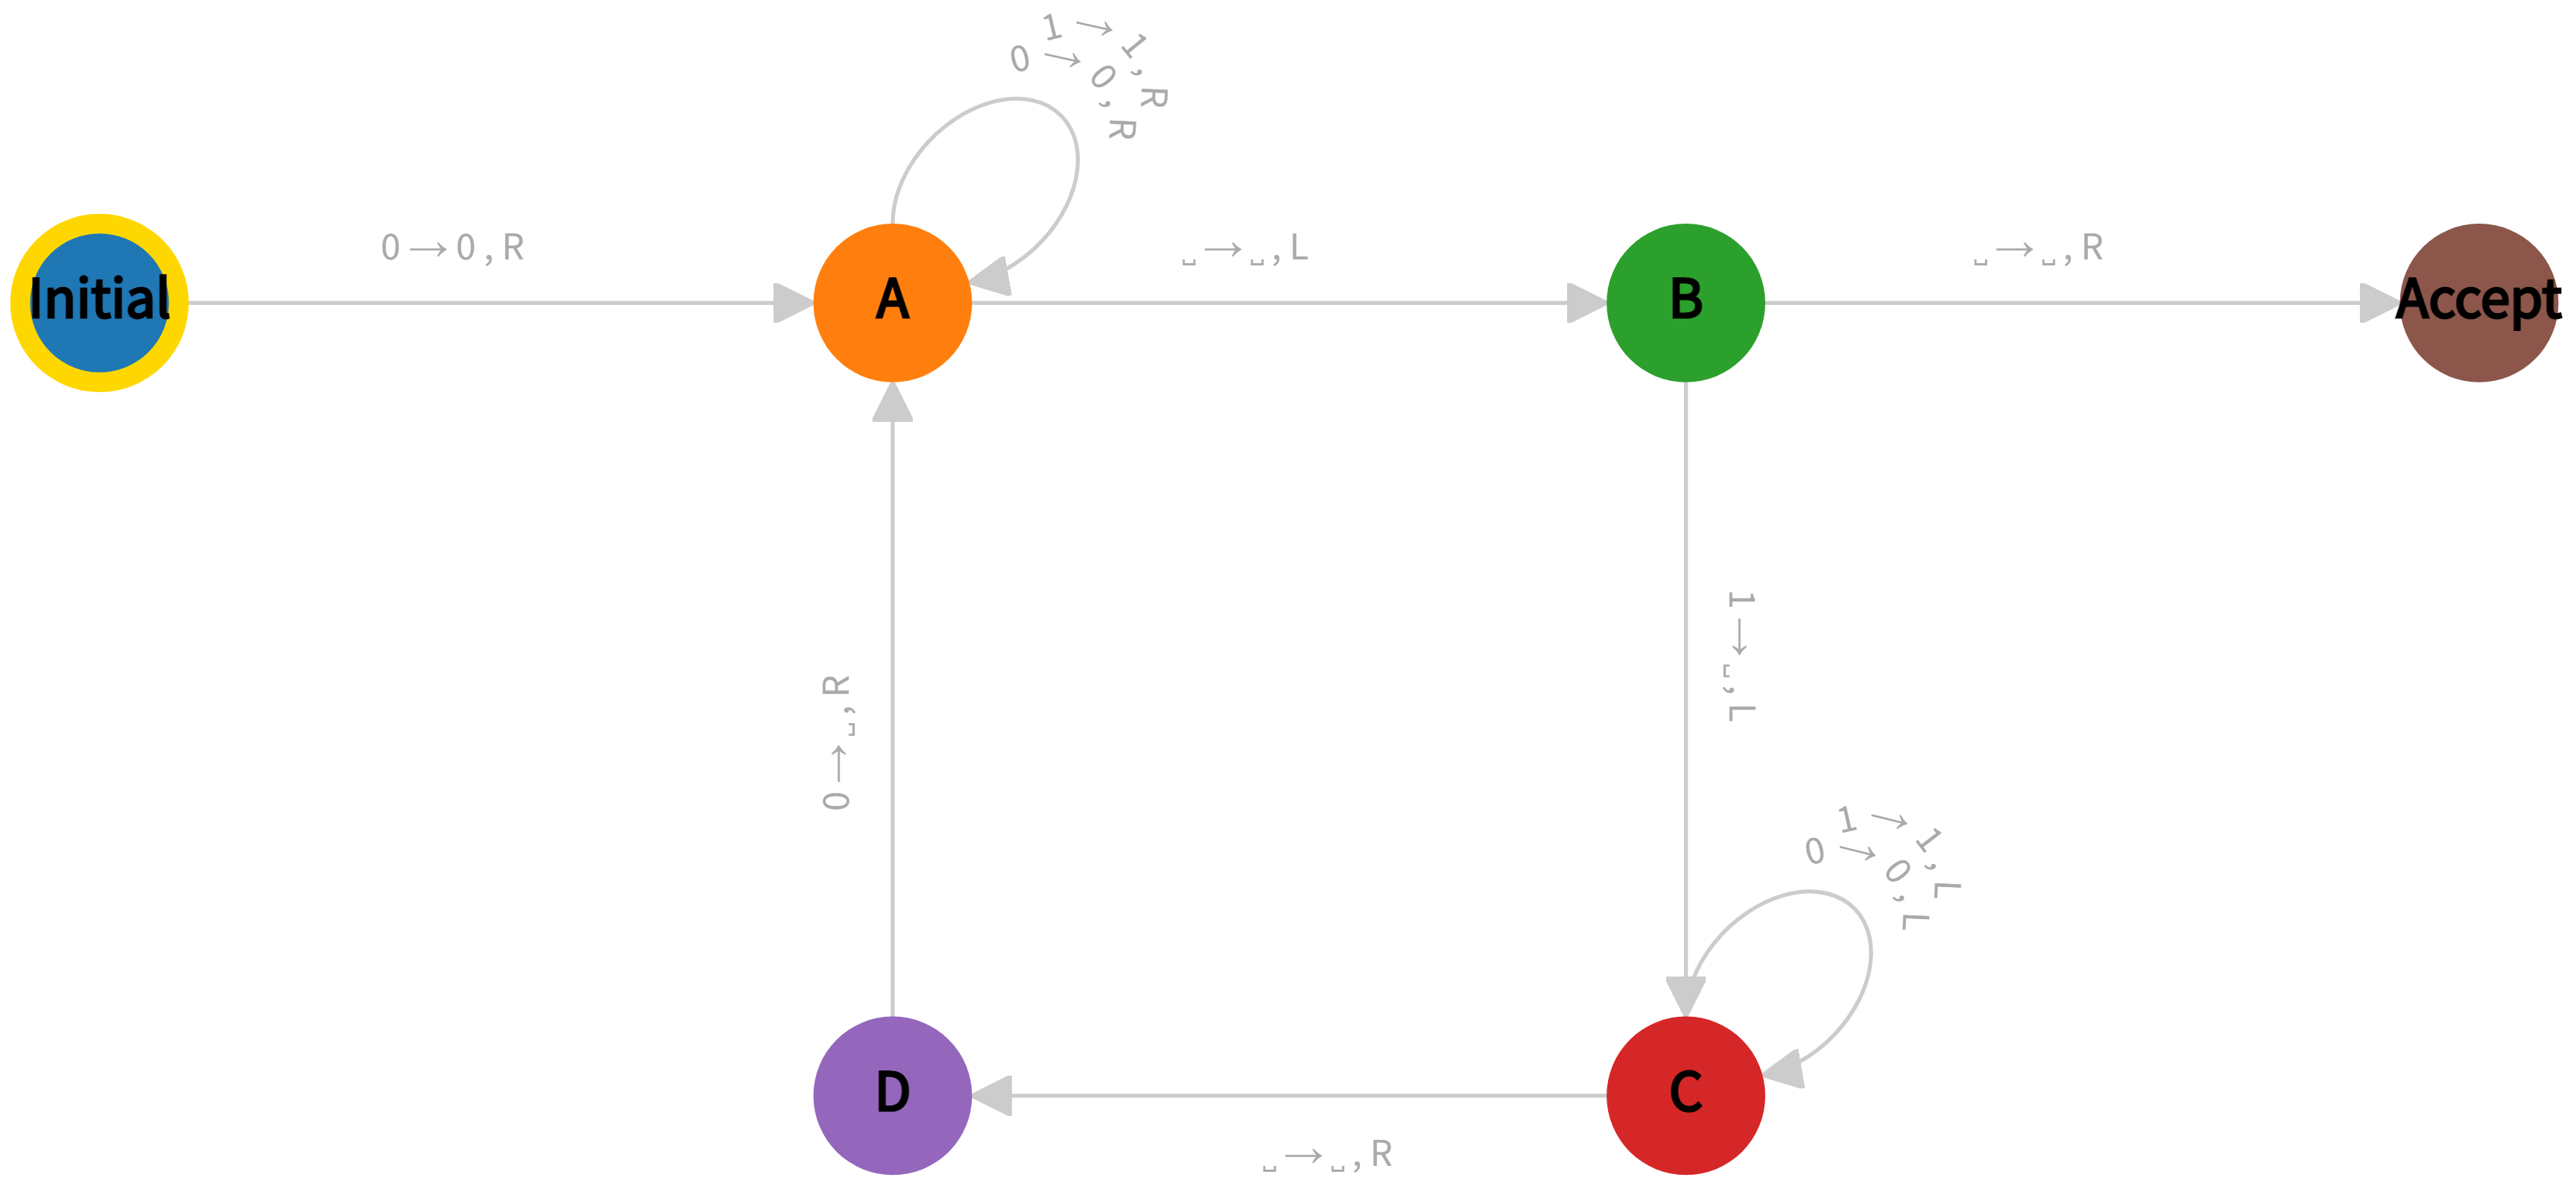
\includegraphics[width=\linewidth]{answers/img/q1-machine.png}
  \caption{\textit{Screenshot of the Turing Machine designed for Q1}}
  \label{fig:q1-machine}
\end{figure}

\begin{center} \subsection*{Descriptions of States} \end{center}
\label{q1:description-of-states}

\subsubsection*{State: Initial}
\label{q1-state:initial}

\textit{It is the start state}. If string starts with $\mathbf{1}$ or $\blank$, machine immediately stops in this state. If string starts with $\mathbf{0}$, head is moved to $\mathbf{R}$ and state of machine goes to state \hyperref[q1-state:A]{$\mathbf{A}$}.

\subsubsection*{State: A}
\label{q1-state:A}

\textit{It scans to the right for the first $\blank$}.
\begin{itemize}
  \item If $\blank$ is found, head is moved one left and state of machine goes to state \hyperref[q1-state:B]{$\mathbf{D}$}.
  \item If $\blank$ is not found, head is moved one right and state of machine is still in \hyperref[q1-state:A]{$\mathbf{A}$}.
\end{itemize}

\subsubsection*{State: B}
\label{q1-state:B}

\textit{It is state indicating that the head is in rightmost $\mathbf{1}$ or input is correct and it should be accepted}. 
\begin{itemize}
  \item If $\mathbf{1}$ is read, $\blank$ is written and head is moved to left. State of machine goes to state \hyperref[q1-state:C]{$\mathbf{C}$}.
  \item If $\blank$ is read, it indicates that the input is correct and should be accepted. Therefore, state of machine goes to state \hyperref[q1-state:Accept]{$\mathbf{Accept}$}.
\end{itemize}

\subsubsection*{State: C}
\label{q1-state:C}

\textit{It scans to the left for the first $\blank$}.
\begin{itemize}
  \item If $\blank$ is found, head is moved one right and state of machine goes to state \hyperref[q1-state:D]{$\mathbf{D}$}.
  \item If $\blank$ is not found, head is moved one left and state of machine is still in \hyperref[q1-state:C]{$\mathbf{C}$}.
\end{itemize}

\subsubsection*{State: D}
\label{q1-state:D}

\textit{It is state indicating that the head is in leftmost $\mathbf{0}$}. 
\begin{itemize}
  \item If $\mathbf{0}$ is read, $\blank$ is written and head is moved to right. State of machine goes to state \hyperref[q1-state:A]{$\mathbf{A}$}.
  \item If $\mathbf{0}$ is not read, it indicates that the input is not correct and shouldn't be accepted. Therefore, state of machine is not changed and crash.
\end{itemize}

\subsubsection*{State: Accept}
\label{q1-state:Accept}

\textit{It is state indicating that the input is correct and accepted}. Therefore, the machine stops, successfully.

\newpage 

\begin{center} \subsection*{Input Samples} \end{center}
\label{q1:input-samples}

\vspace*{\fill}

\subsubsection*{Input: 000111 $|$ Accept}
\label{q1-000111}

\begin{figure}[ht]
  \centering
  \begin{minipage}{.49\linewidth}
    \centering
    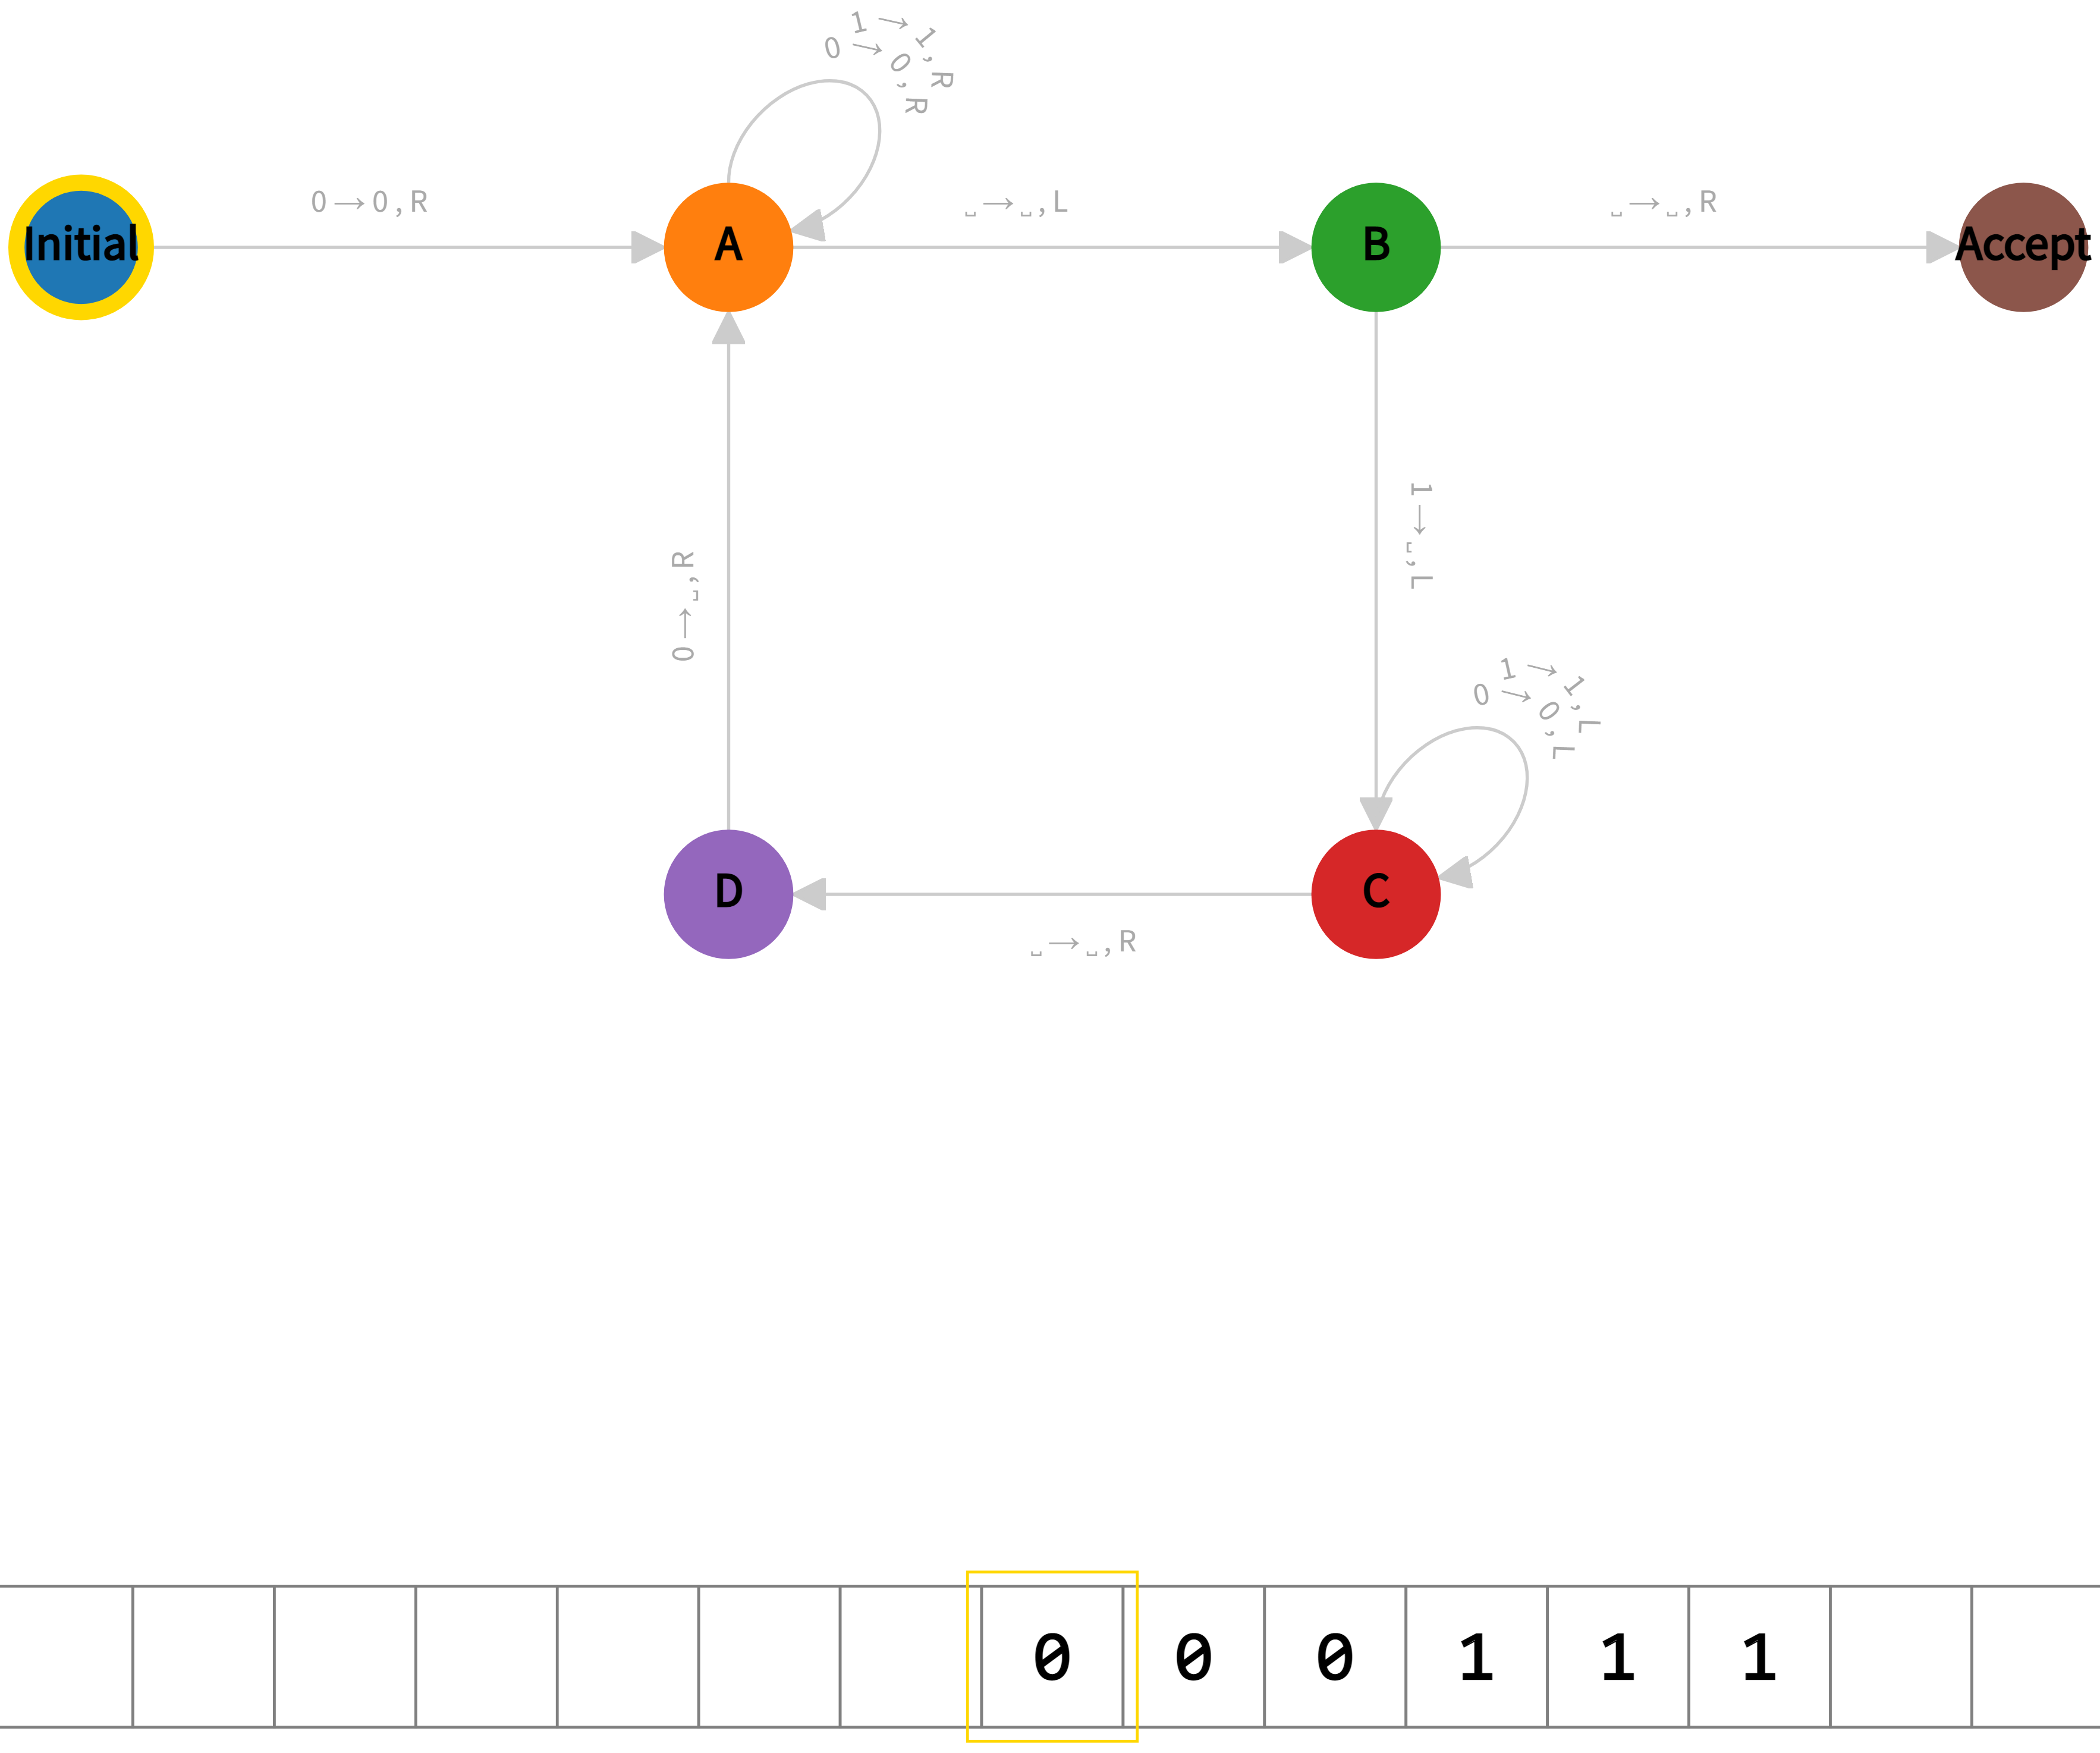
\includegraphics[width=\linewidth]{answers/img/q1-000111-initial.png}
    \caption*{Figure (a): Initial State for $\mathbf{000111}$}
    \label{fig:000111-initial}
  \end{minipage}
  \begin{minipage}{.49\linewidth}
    \centering
    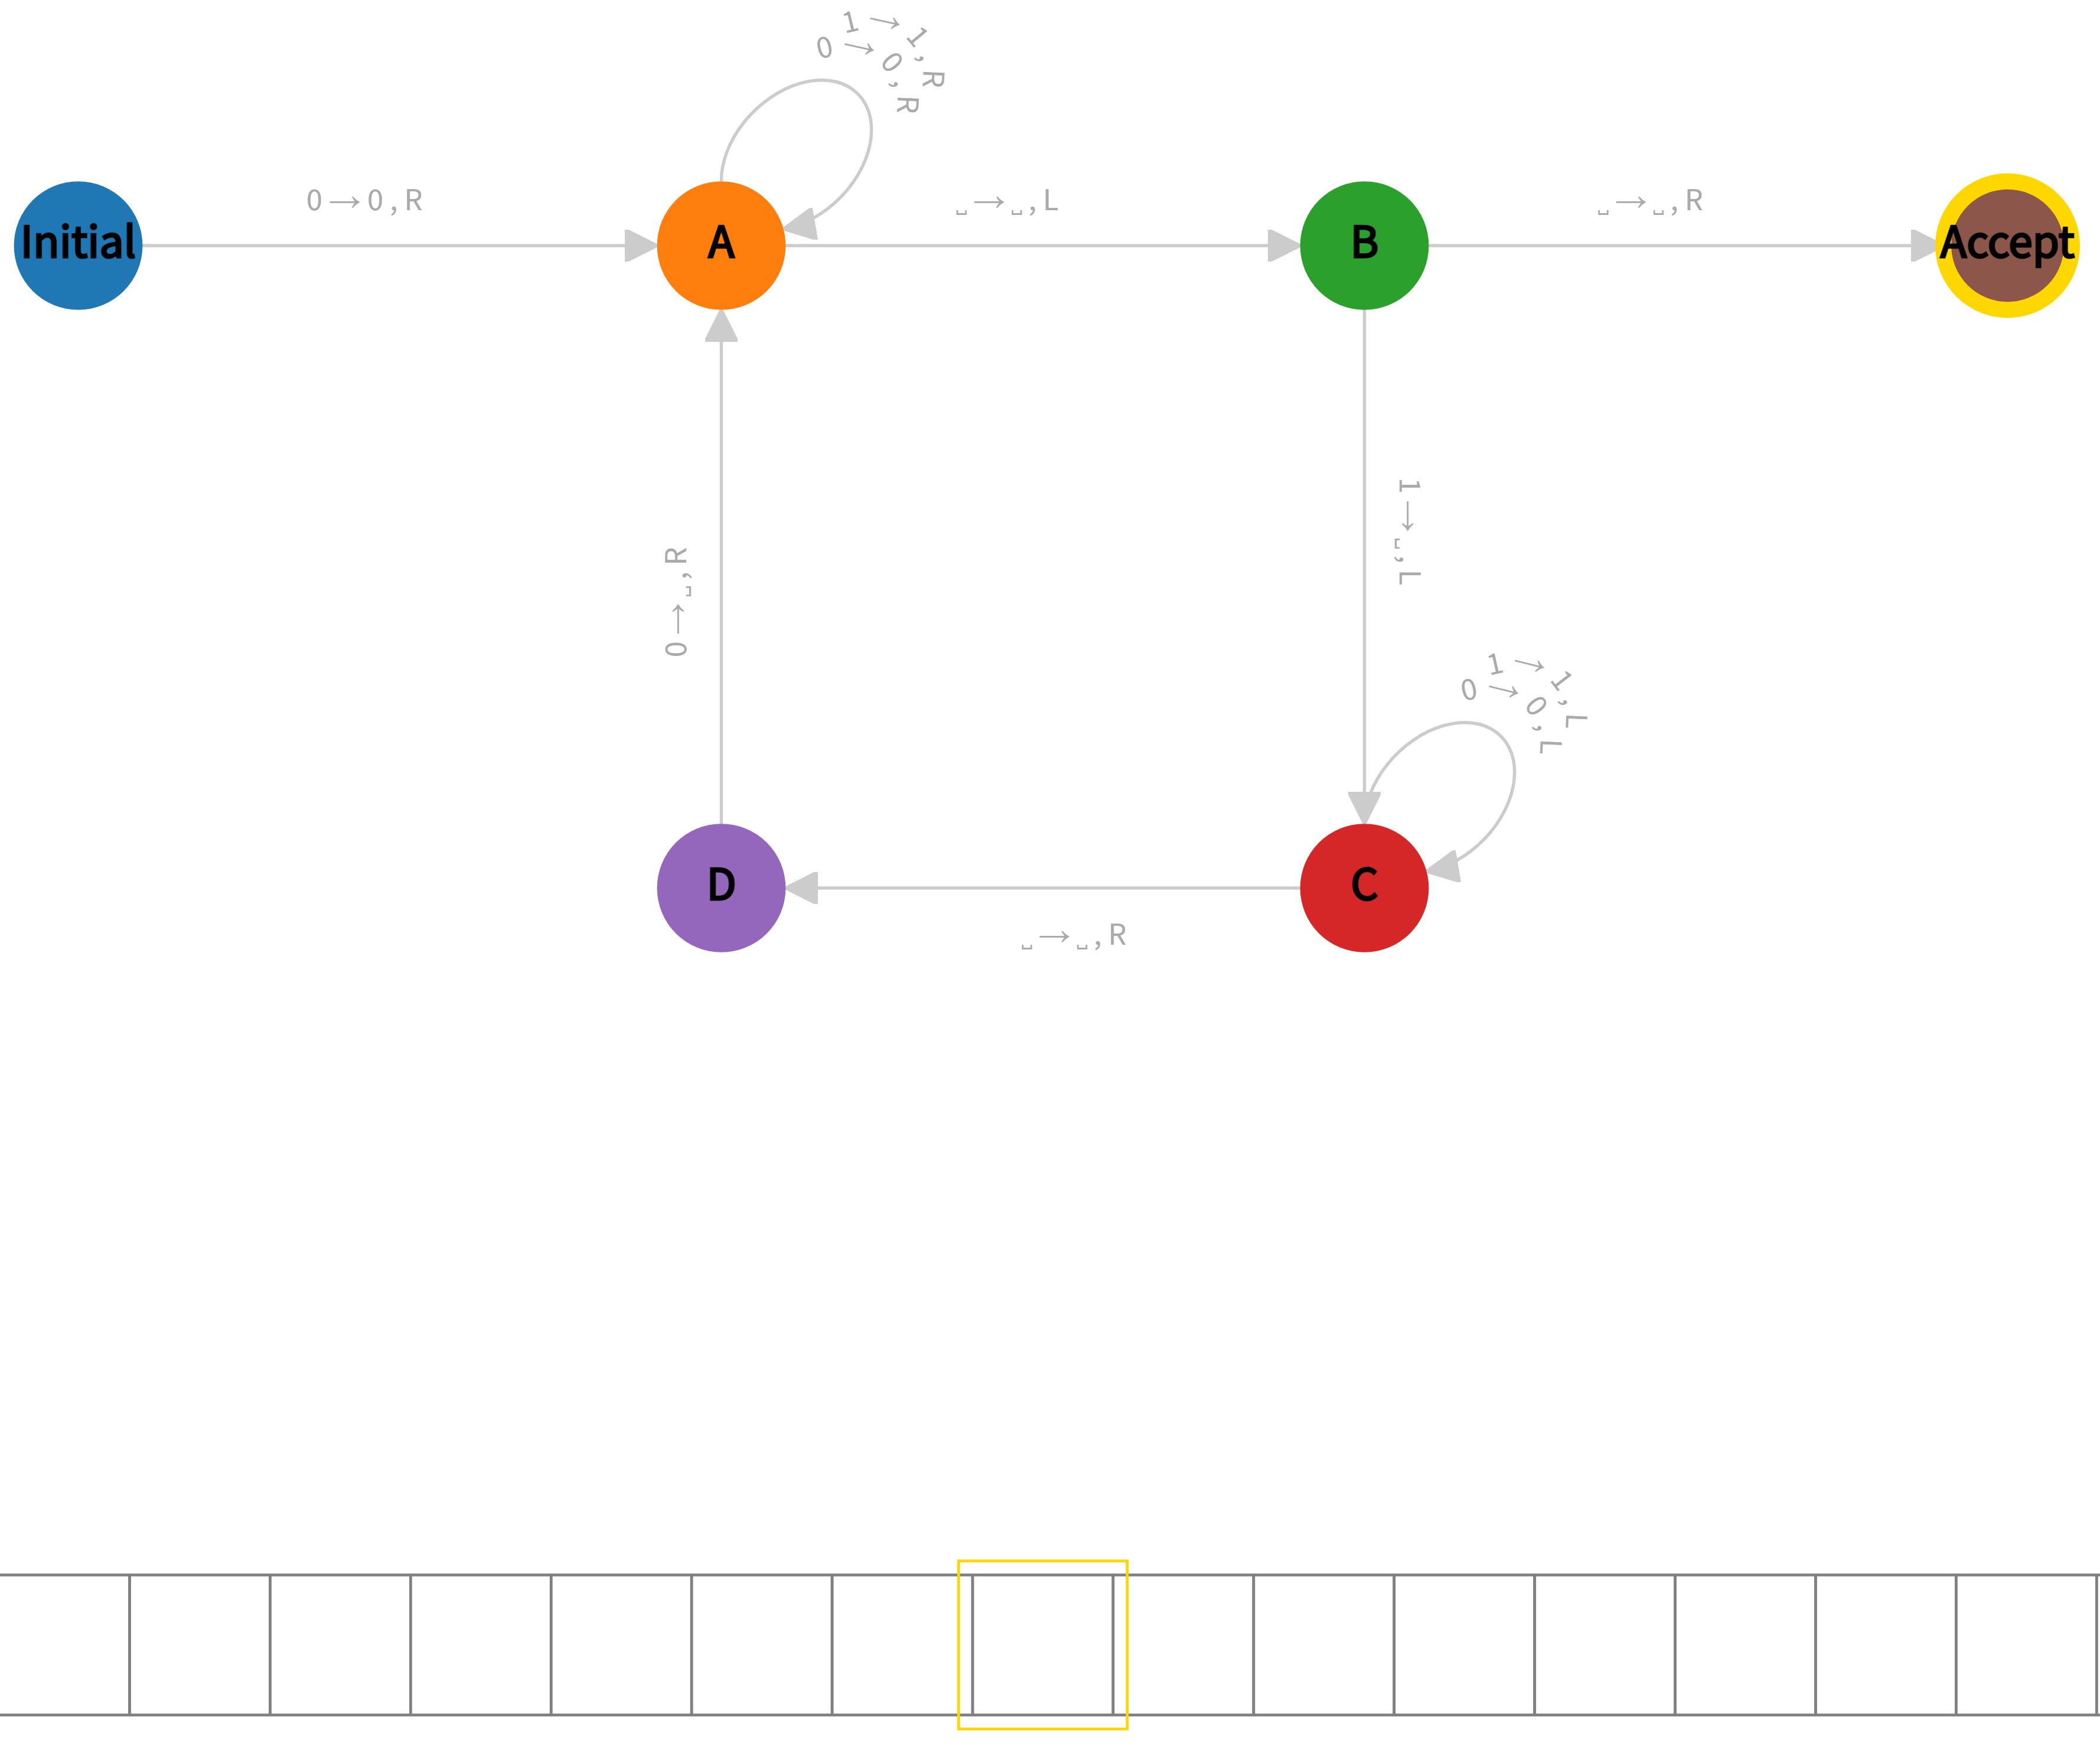
\includegraphics[width=\linewidth]{answers/img/q1-000111-end.png}
    \caption*{Figure (b): End State for $\mathbf{000111}$}
    \label{fig:000111-end}
  \end{minipage}
  \caption{States for $\mathbf{000111}$}
  \label{fig:in-000111}
\end{figure}

\subsubsection*{Input: 0000111 $|$ Reject}
\label{q1-0000111}

\begin{figure}[ht]
  \centering
  \begin{minipage}{.49\linewidth}
    \centering
    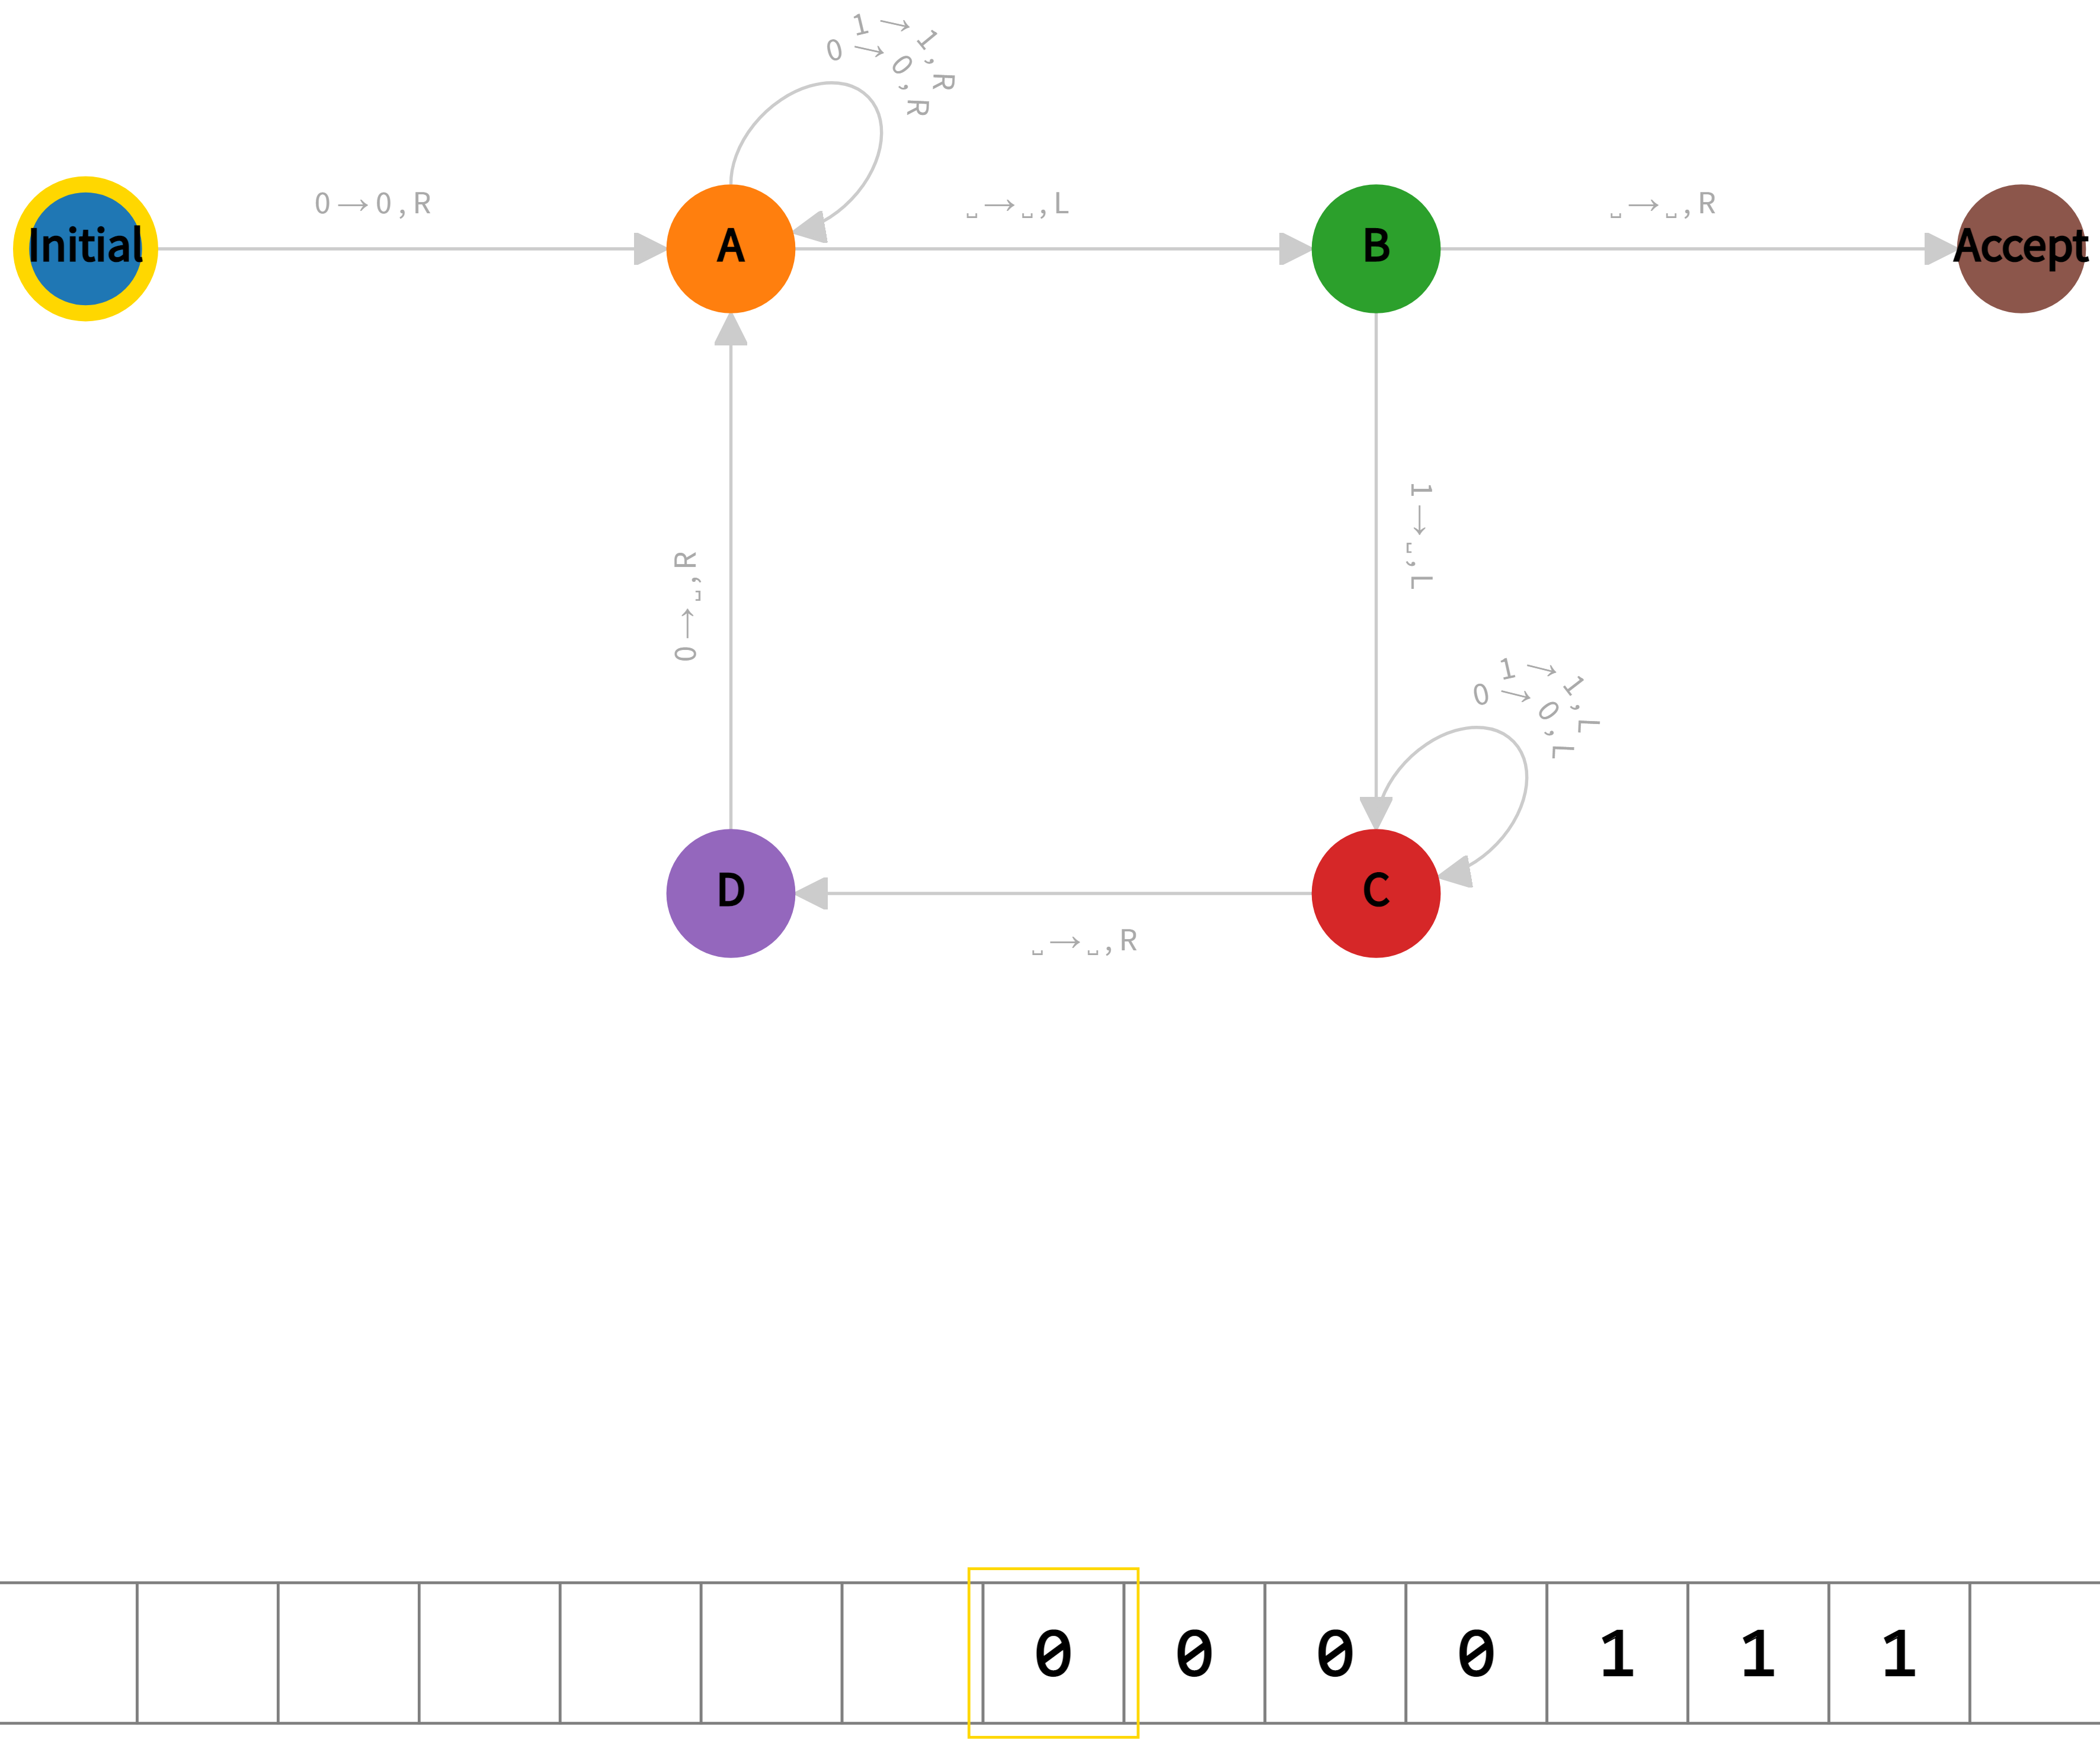
\includegraphics[width=\linewidth]{answers/img/q1-0000111-initial.png}
    \caption*{Figure (a): Initial State for $\mathbf{0000111}$}
    \label{fig:0000111-initial}
  \end{minipage}
  \begin{minipage}{.49\linewidth}
    \centering
    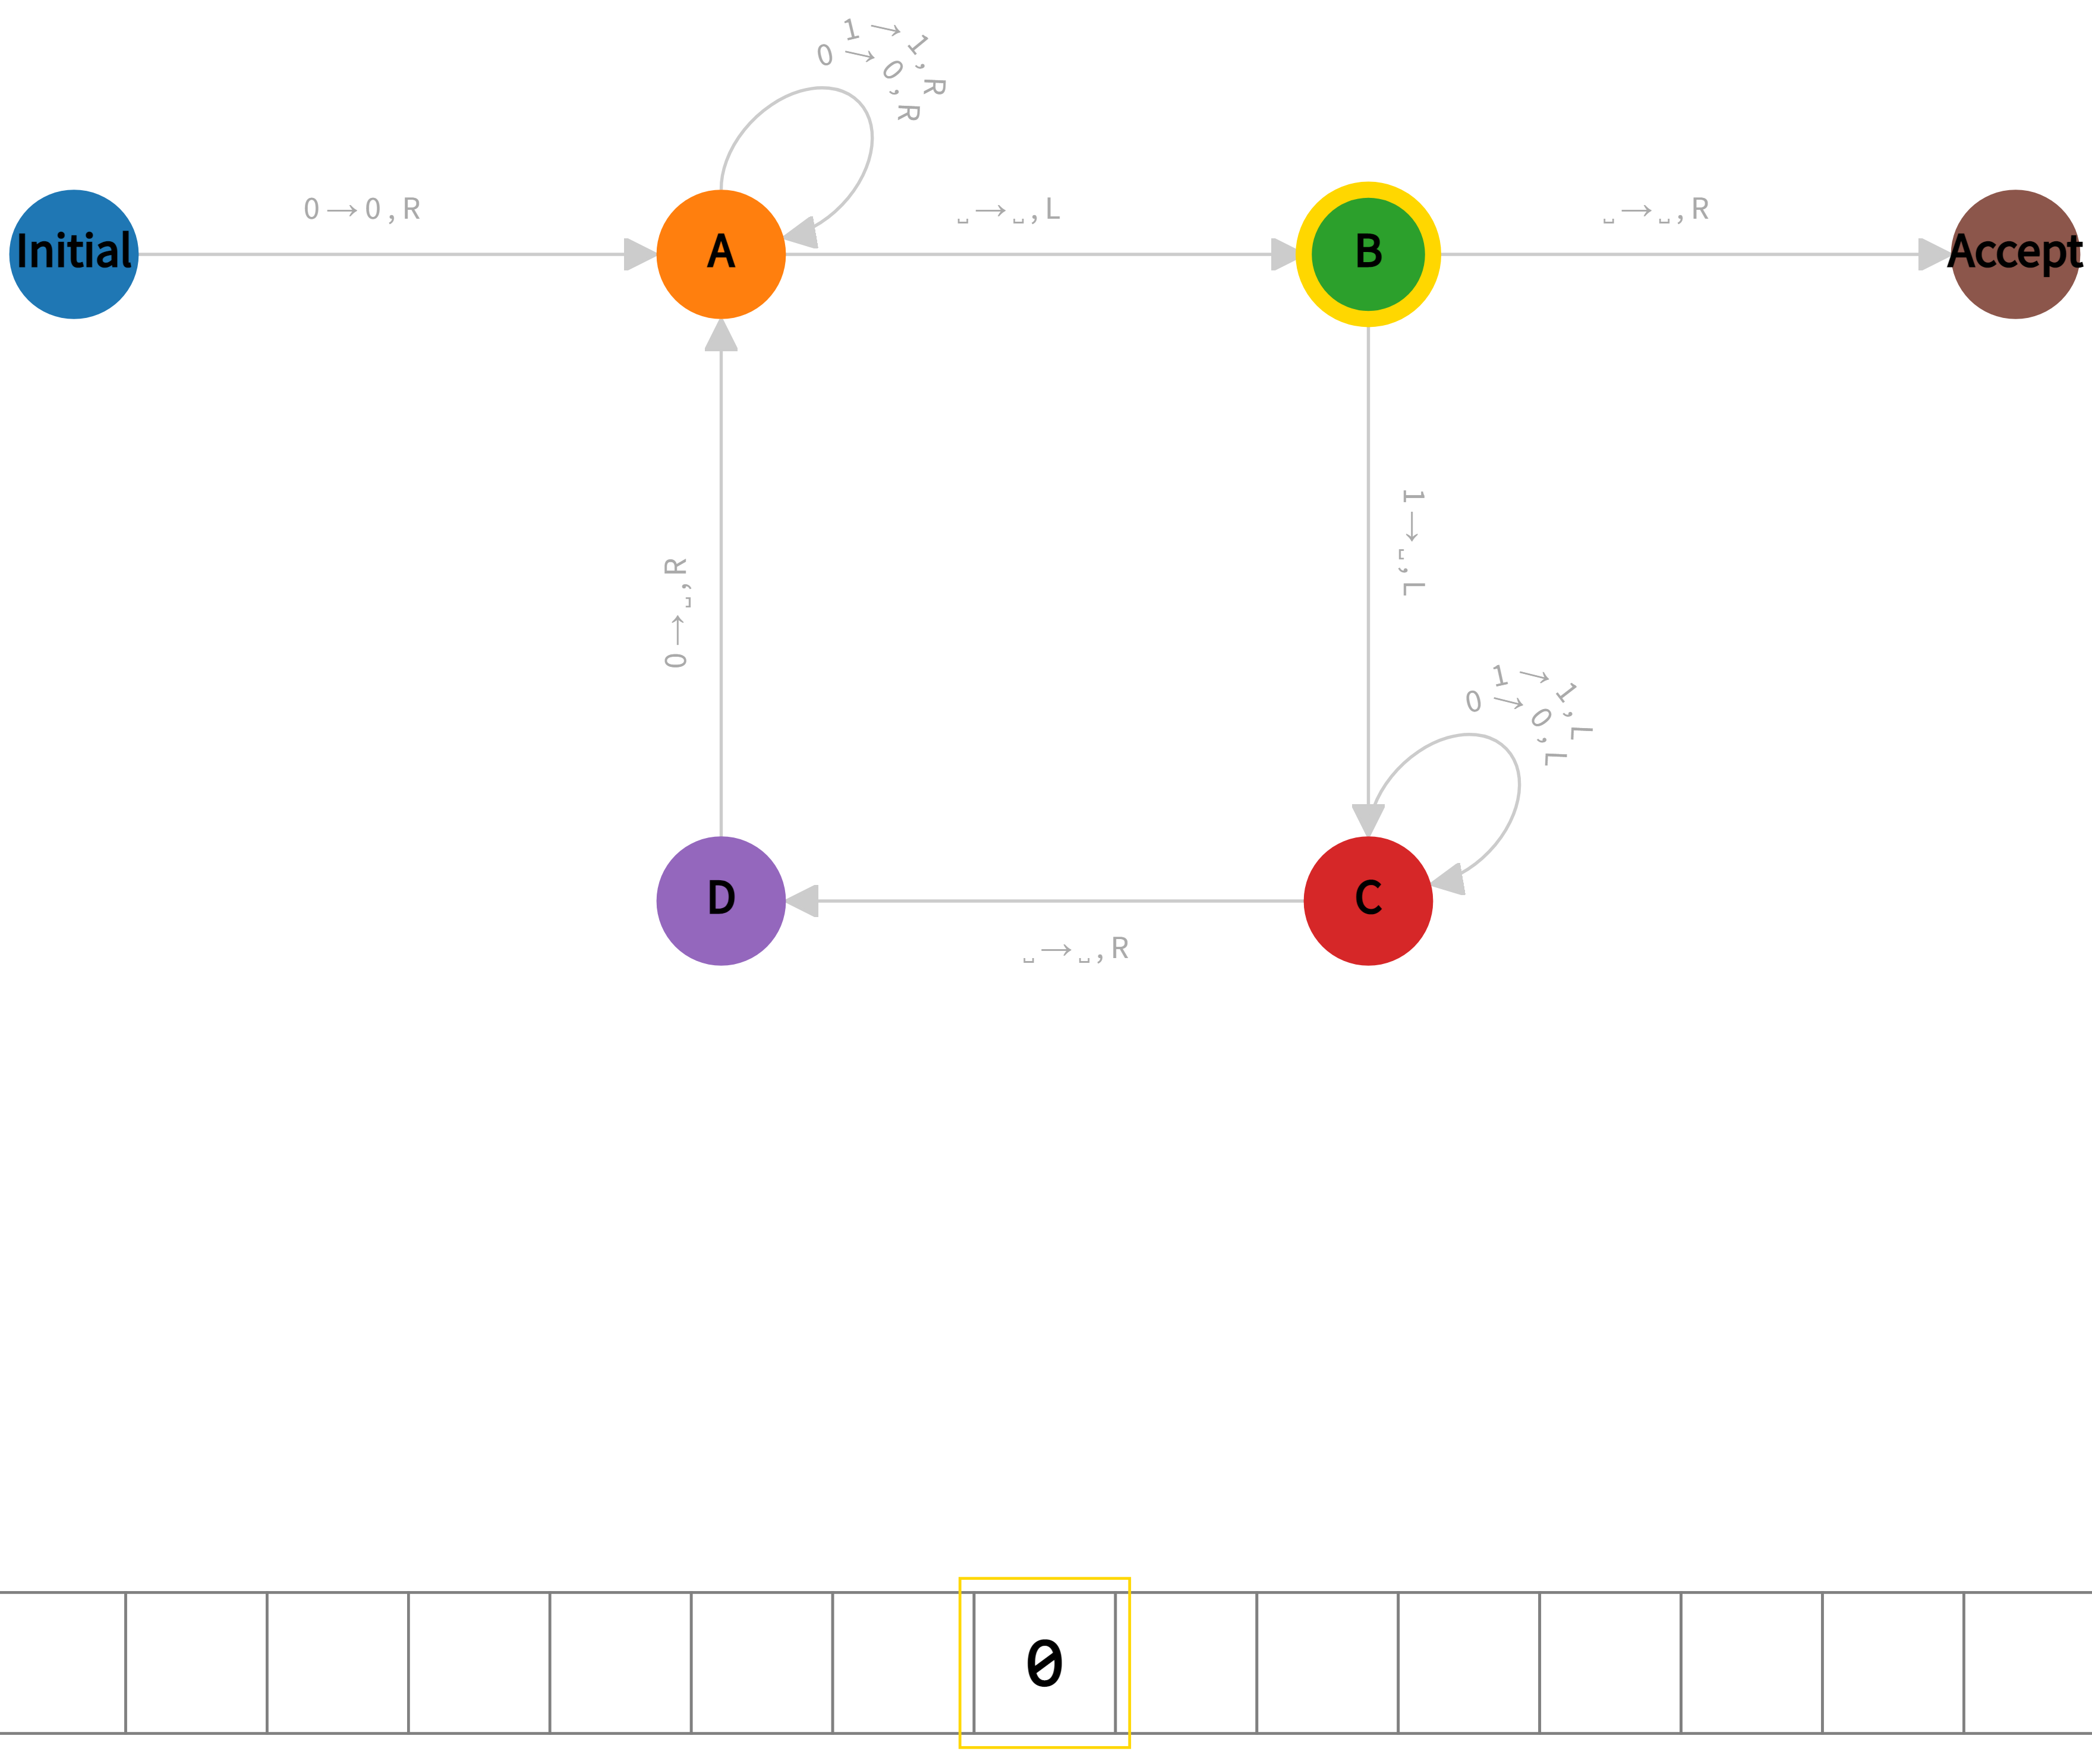
\includegraphics[width=\linewidth]{answers/img/q1-0000111-end.png}
    \caption*{Figure (b): End State for $\mathbf{0000111}$}
    \label{fig:0000111-end}
  \end{minipage}
  \caption{States for $\mathbf{0000111}$}
  \label{fig:in-0000111}
\end{figure}

\vspace*{\fill}
\newpage
\vspace*{\fill}

\subsubsection*{Input: 000011111 $|$ Reject}
\label{q1-000011111}

\begin{figure}[ht]
  \centering
  \begin{minipage}{.49\linewidth}
    \centering
    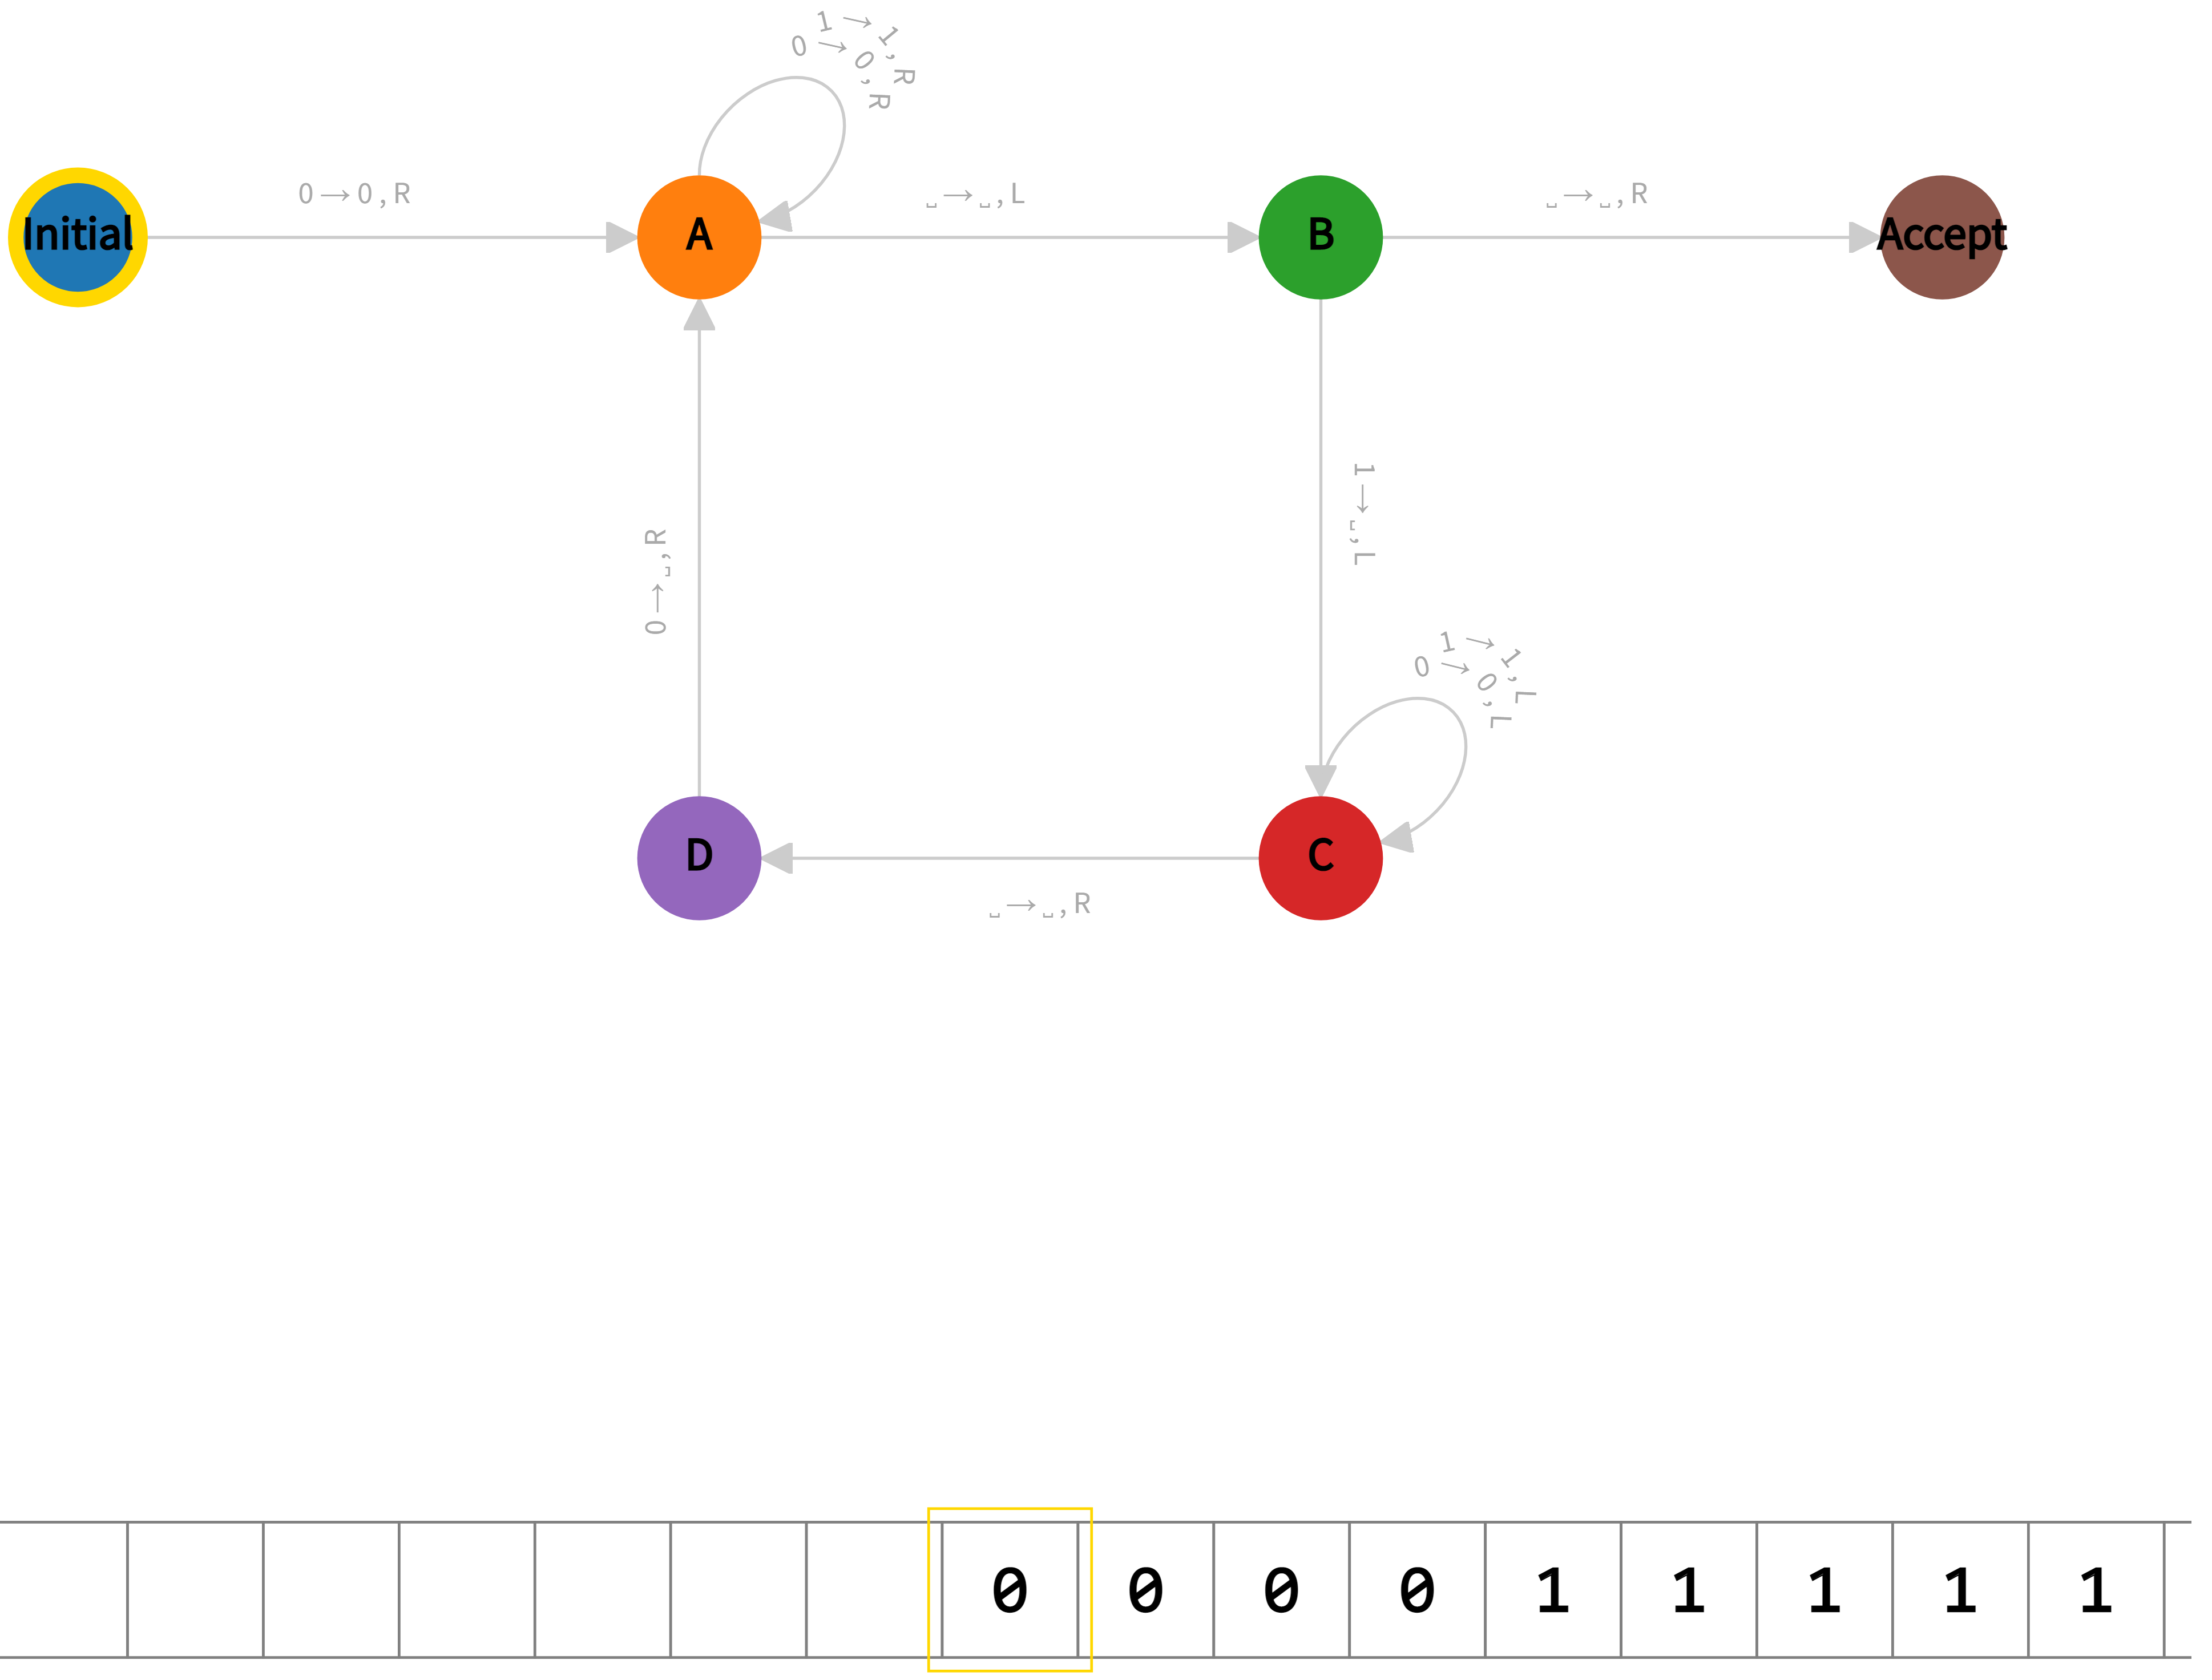
\includegraphics[width=\linewidth]{answers/img/q1-000011111-initial.png}
    \caption*{Figure (a): Initial State for $\mathbf{000011111}$}
    \label{fig:000011111-initial}
  \end{minipage}
  \begin{minipage}{.49\linewidth}
    \centering
    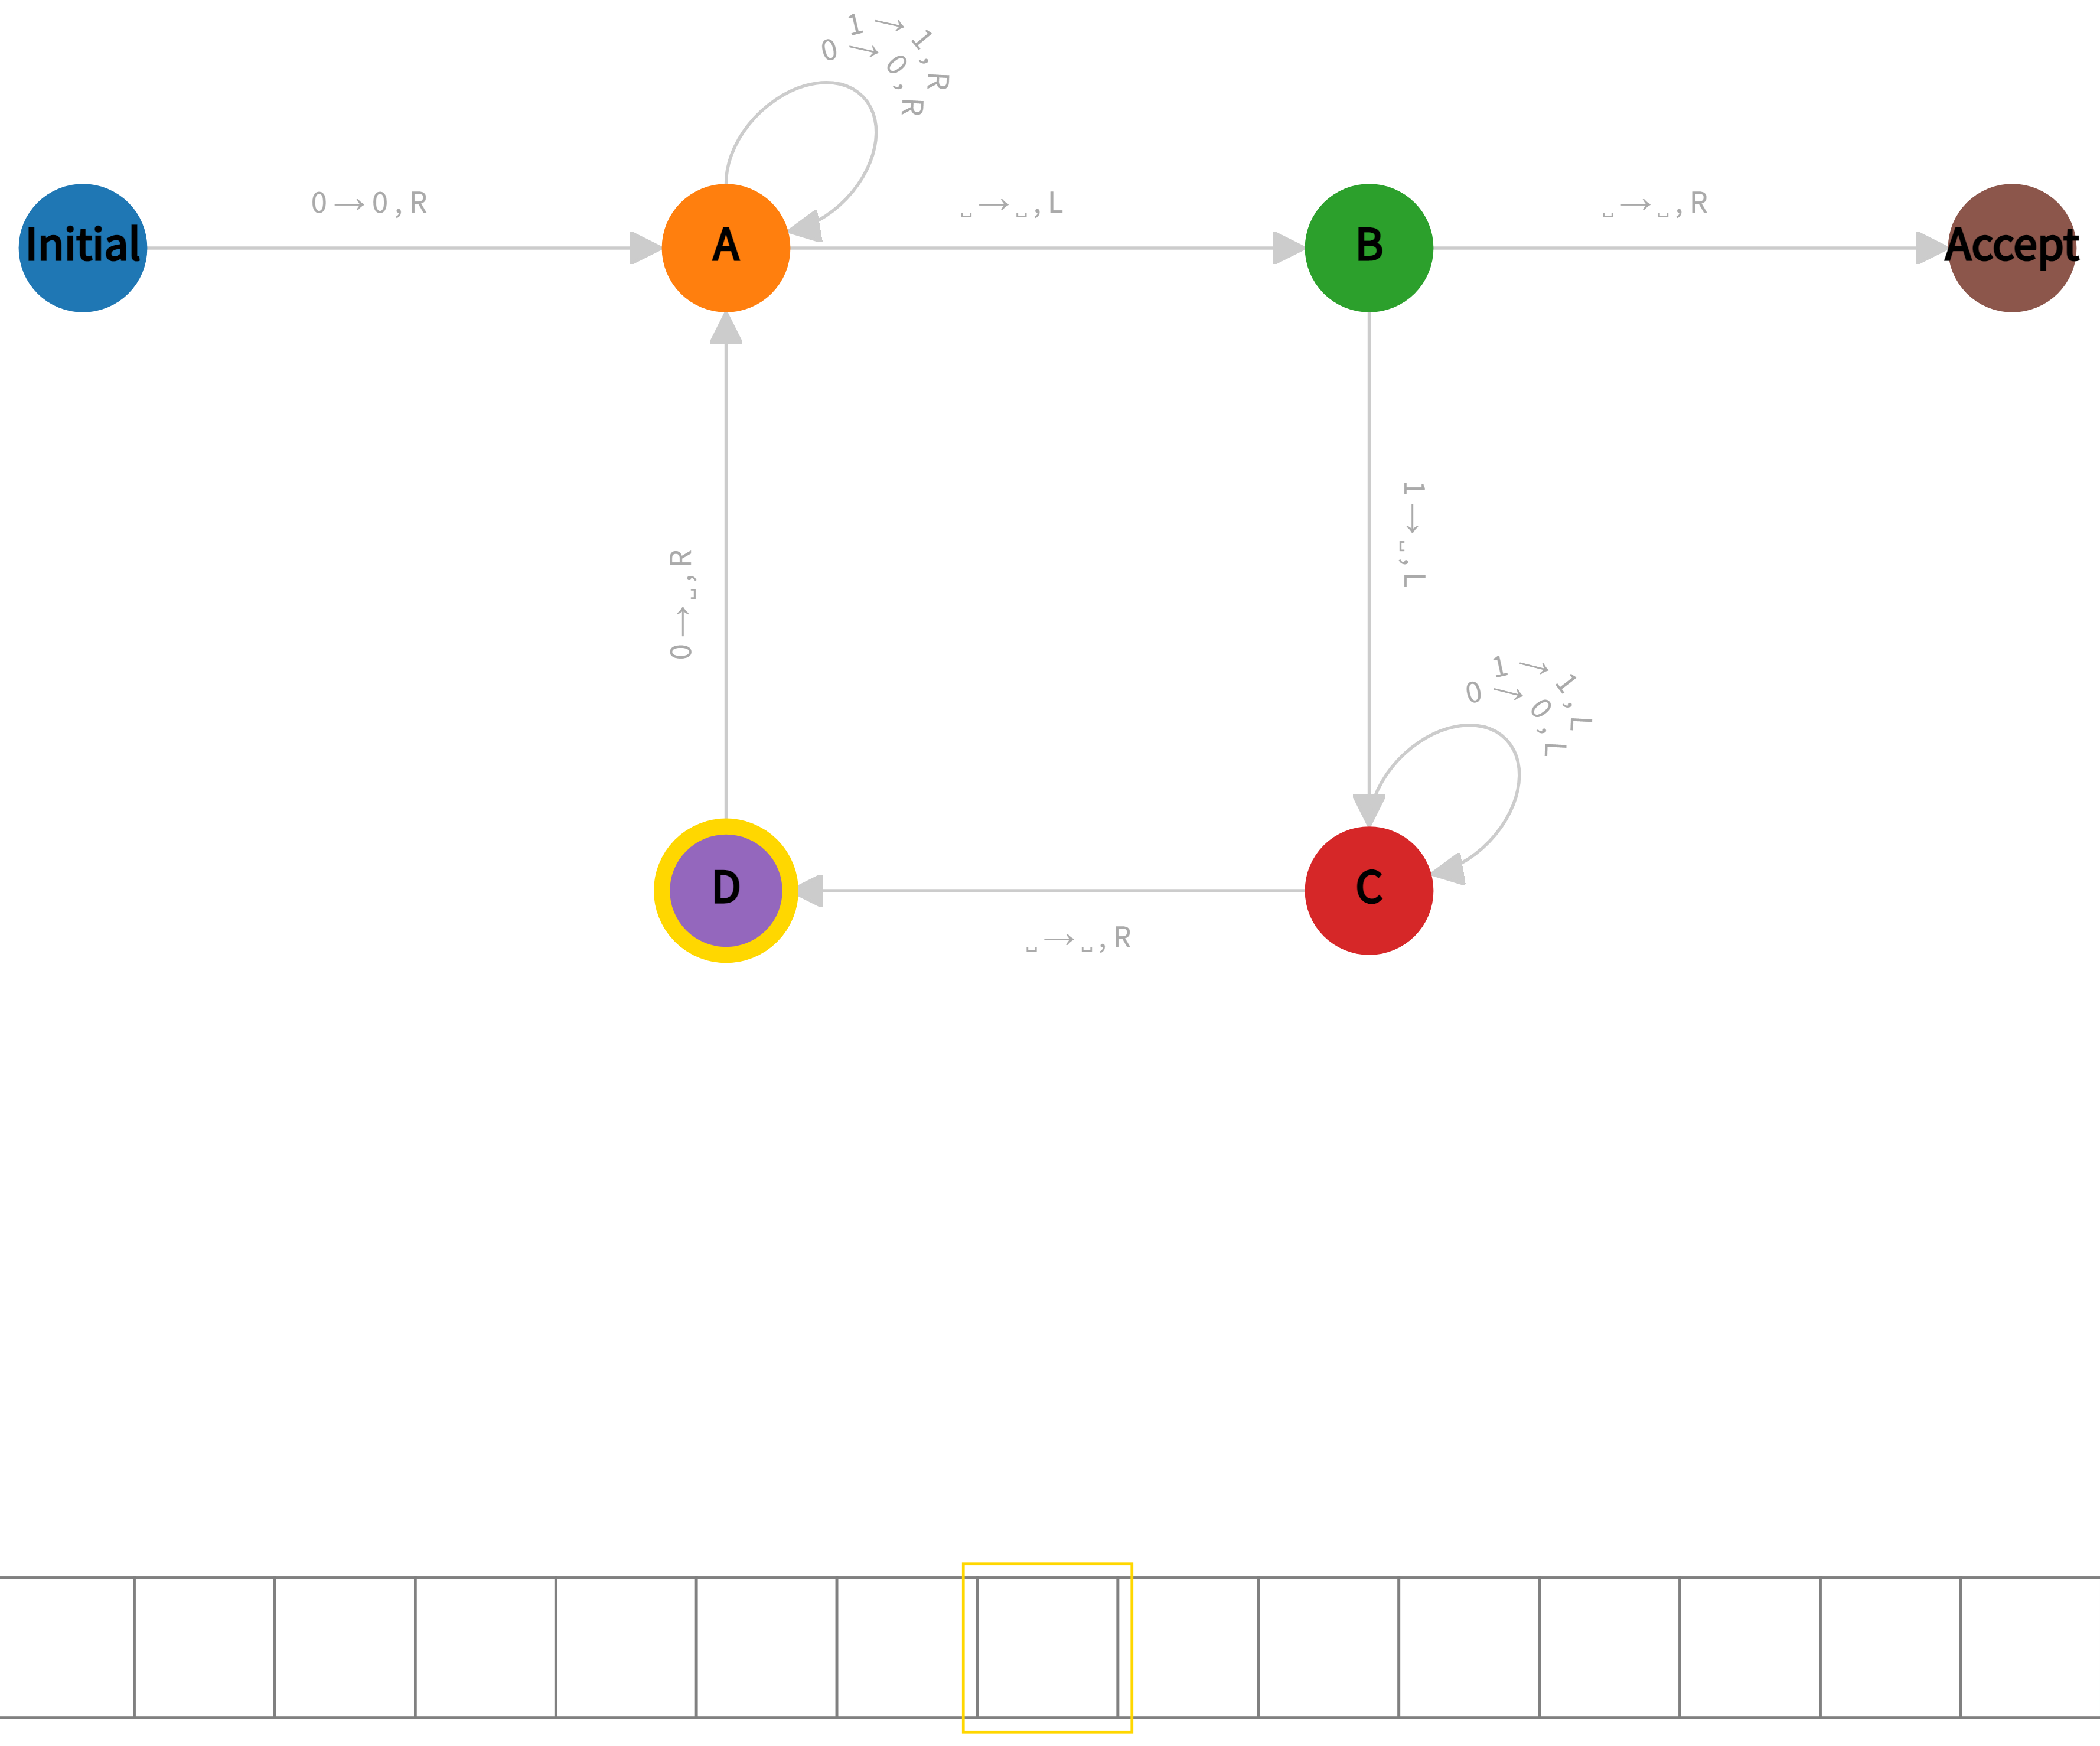
\includegraphics[width=\linewidth]{answers/img/q1-000011111-end.png}
    \caption*{Figure (b): End State for $\mathbf{000011111}$}
    \label{fig:000011111-end}
  \end{minipage}
  \caption{States for $\mathbf{000011111}$}
  \label{fig:in-000011111}
\end{figure}

\subsubsection*{Input: 0001110 $|$ Reject}
\label{q1-0001110}

\begin{figure}[ht]
  \centering
  \begin{minipage}{.49\linewidth}
    \centering
    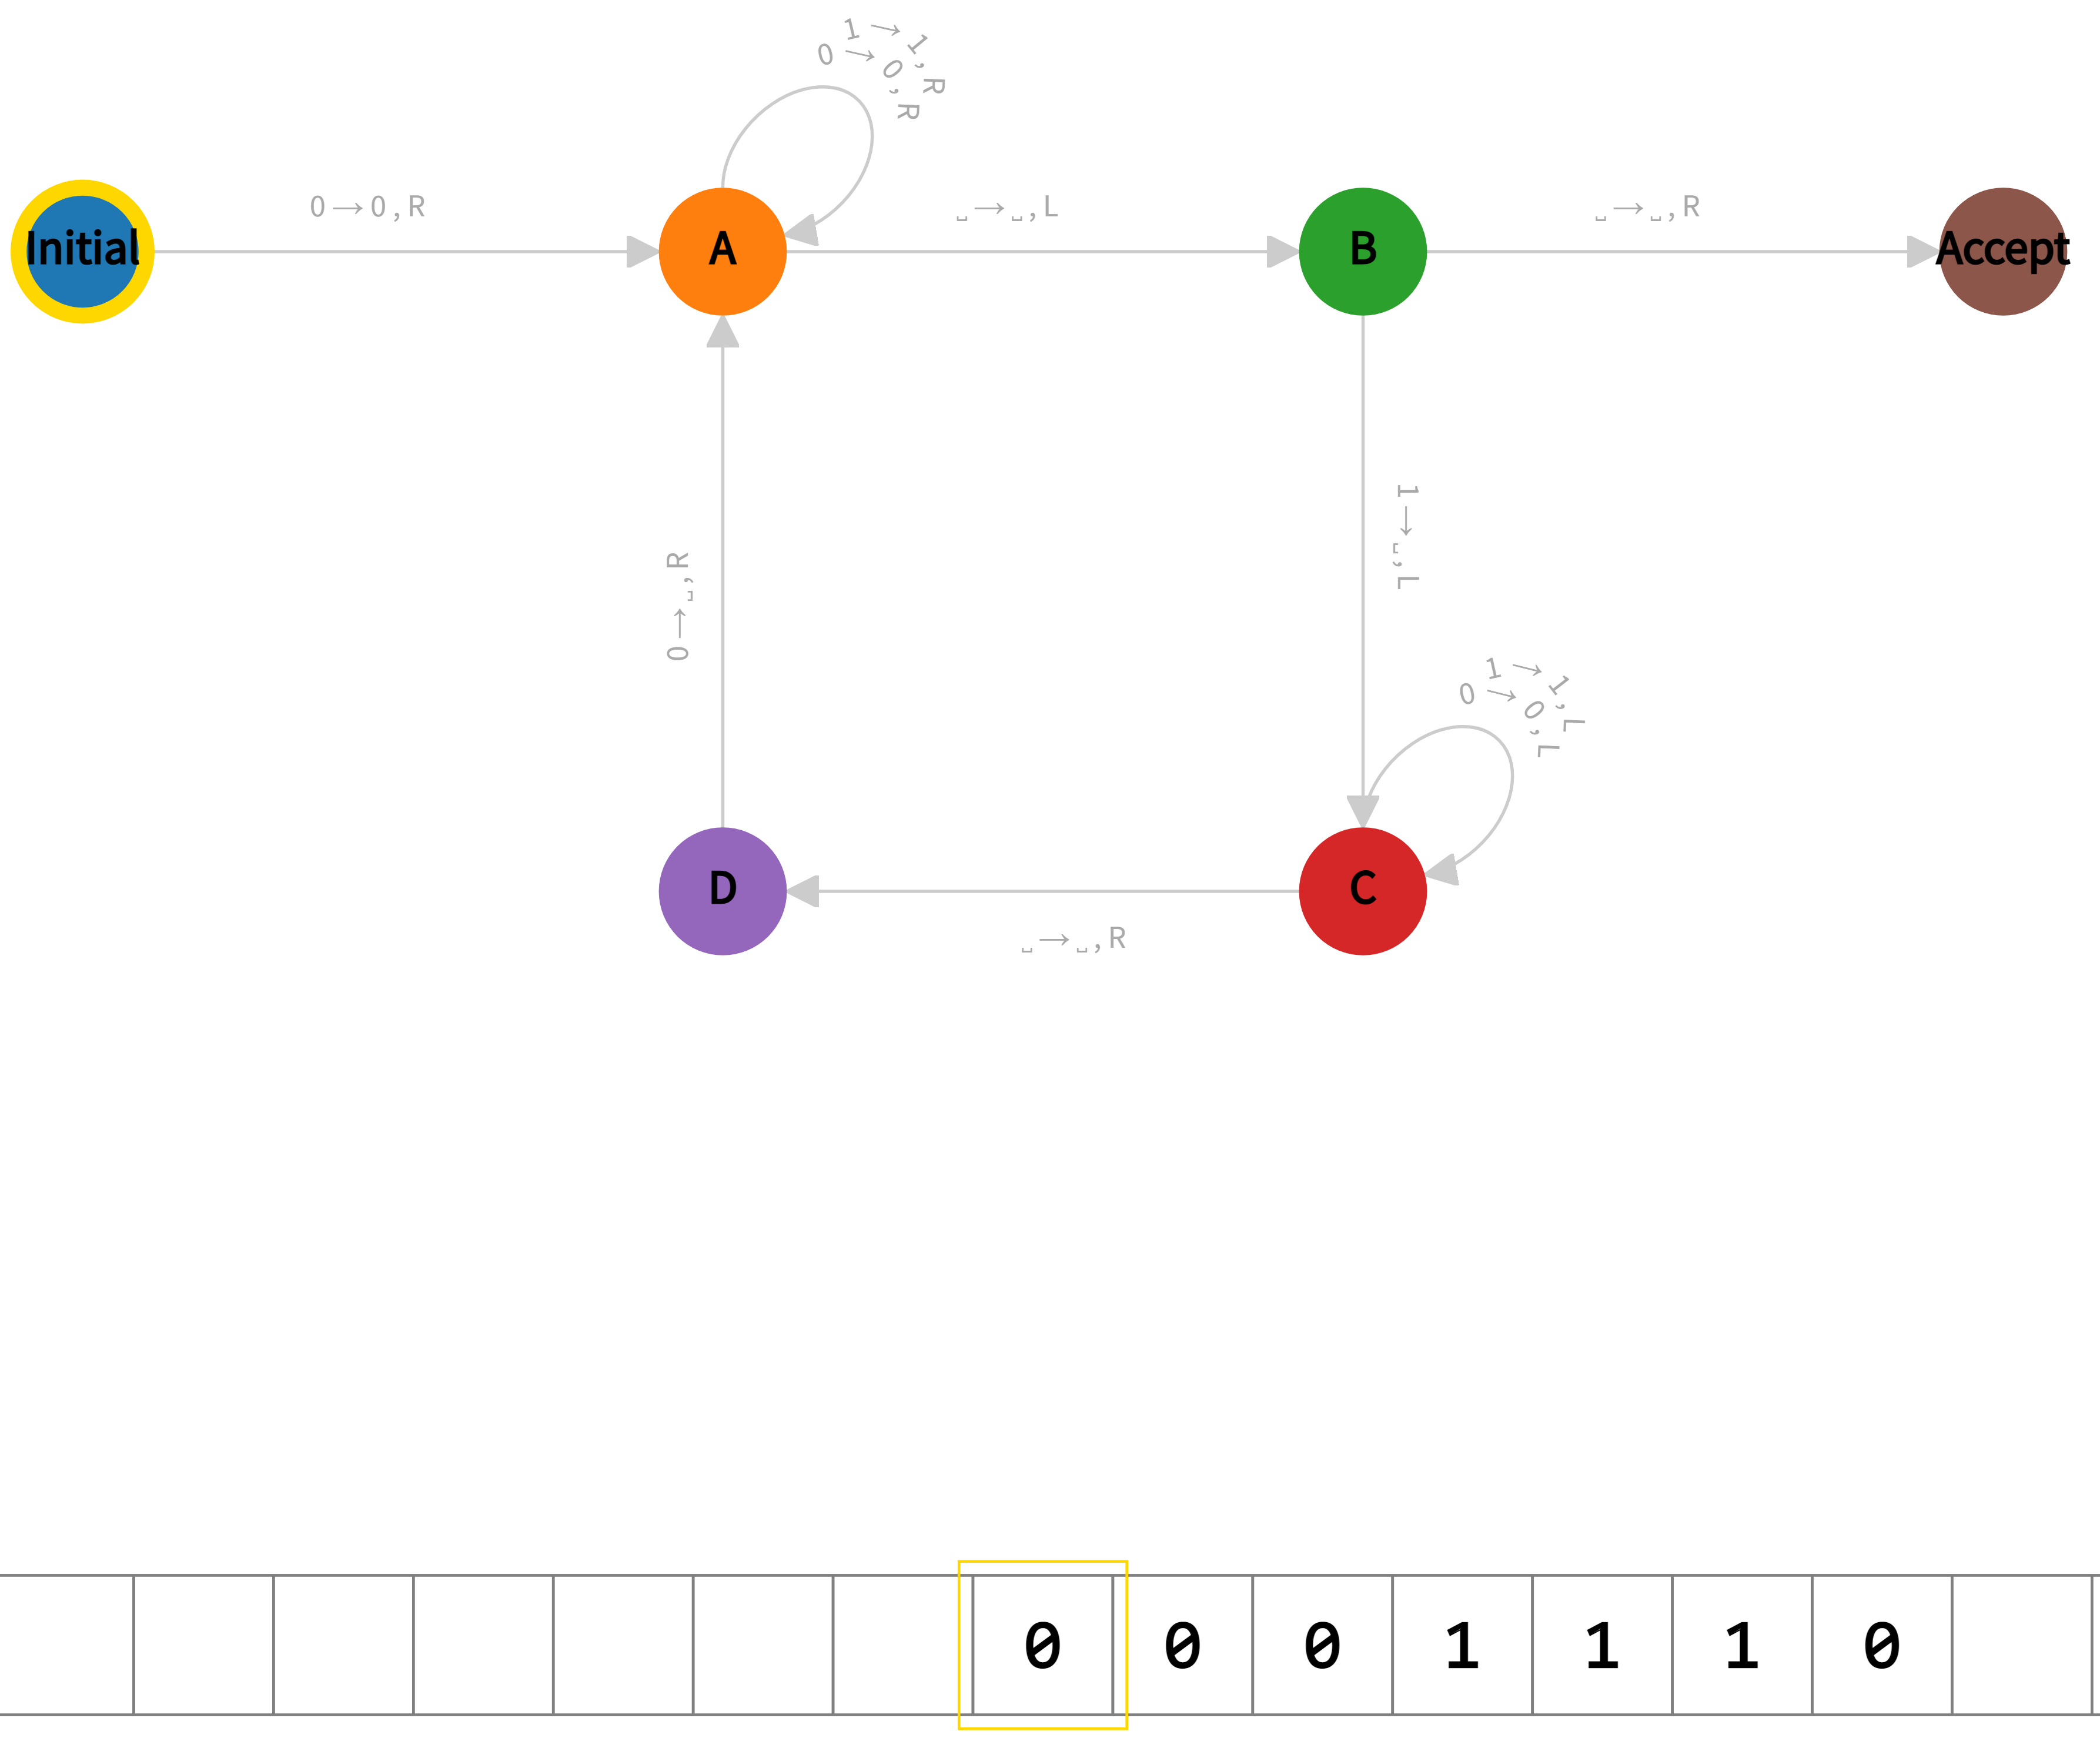
\includegraphics[width=\linewidth]{answers/img/q1-0001110-initial.png}
    \caption*{Figure (a): Initial State for $\mathbf{0001110}$}
    \label{fig:0001110-initial}
  \end{minipage}
  \begin{minipage}{.49\linewidth}
    \centering
    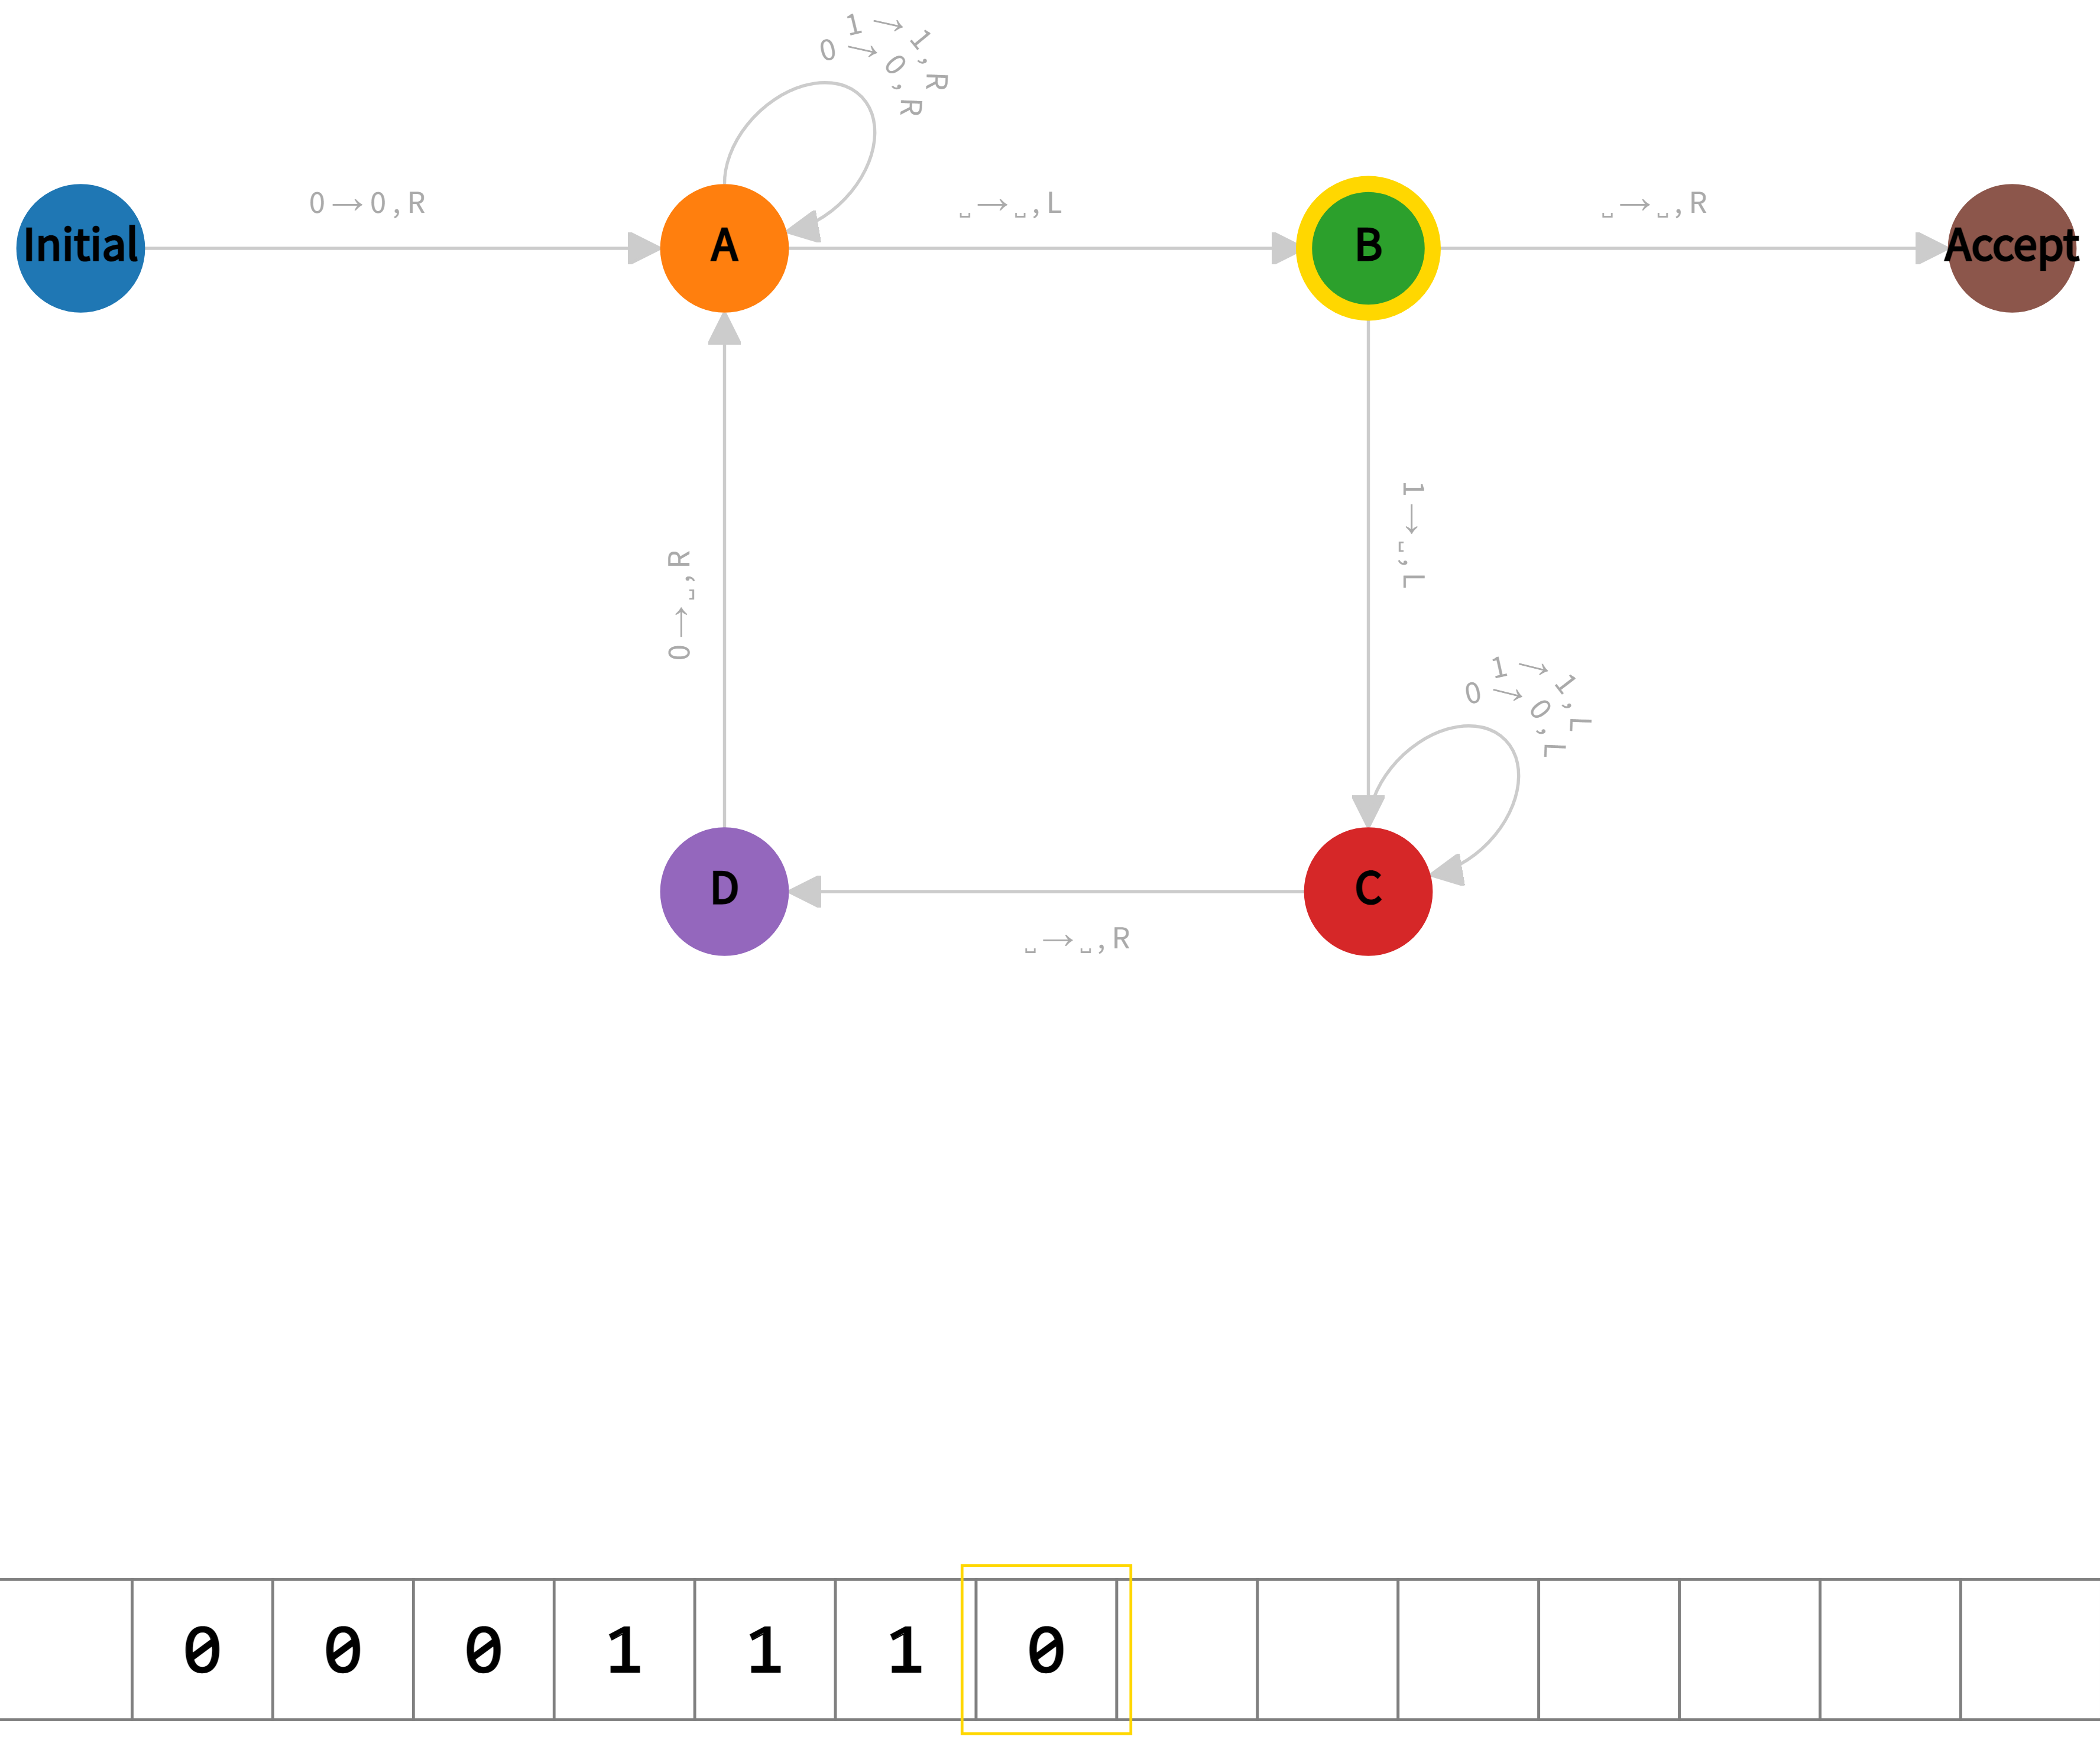
\includegraphics[width=\linewidth]{answers/img/q1-0001110-end.png}
    \caption*{Figure (b): End State for $\mathbf{0001110}$}
    \label{fig:0001110-end}
  \end{minipage}
  \caption{States for $\mathbf{0001110}$}
  \label{fig:in-0001110}
\end{figure}

\vspace*{\fill}
\newpage
\vspace*{\fill}

\subsubsection*{Input: 001101 $|$ Reject}
\label{q1-001101}

\begin{figure}[ht]
  \centering
  \begin{minipage}{.49\linewidth}
    \centering
    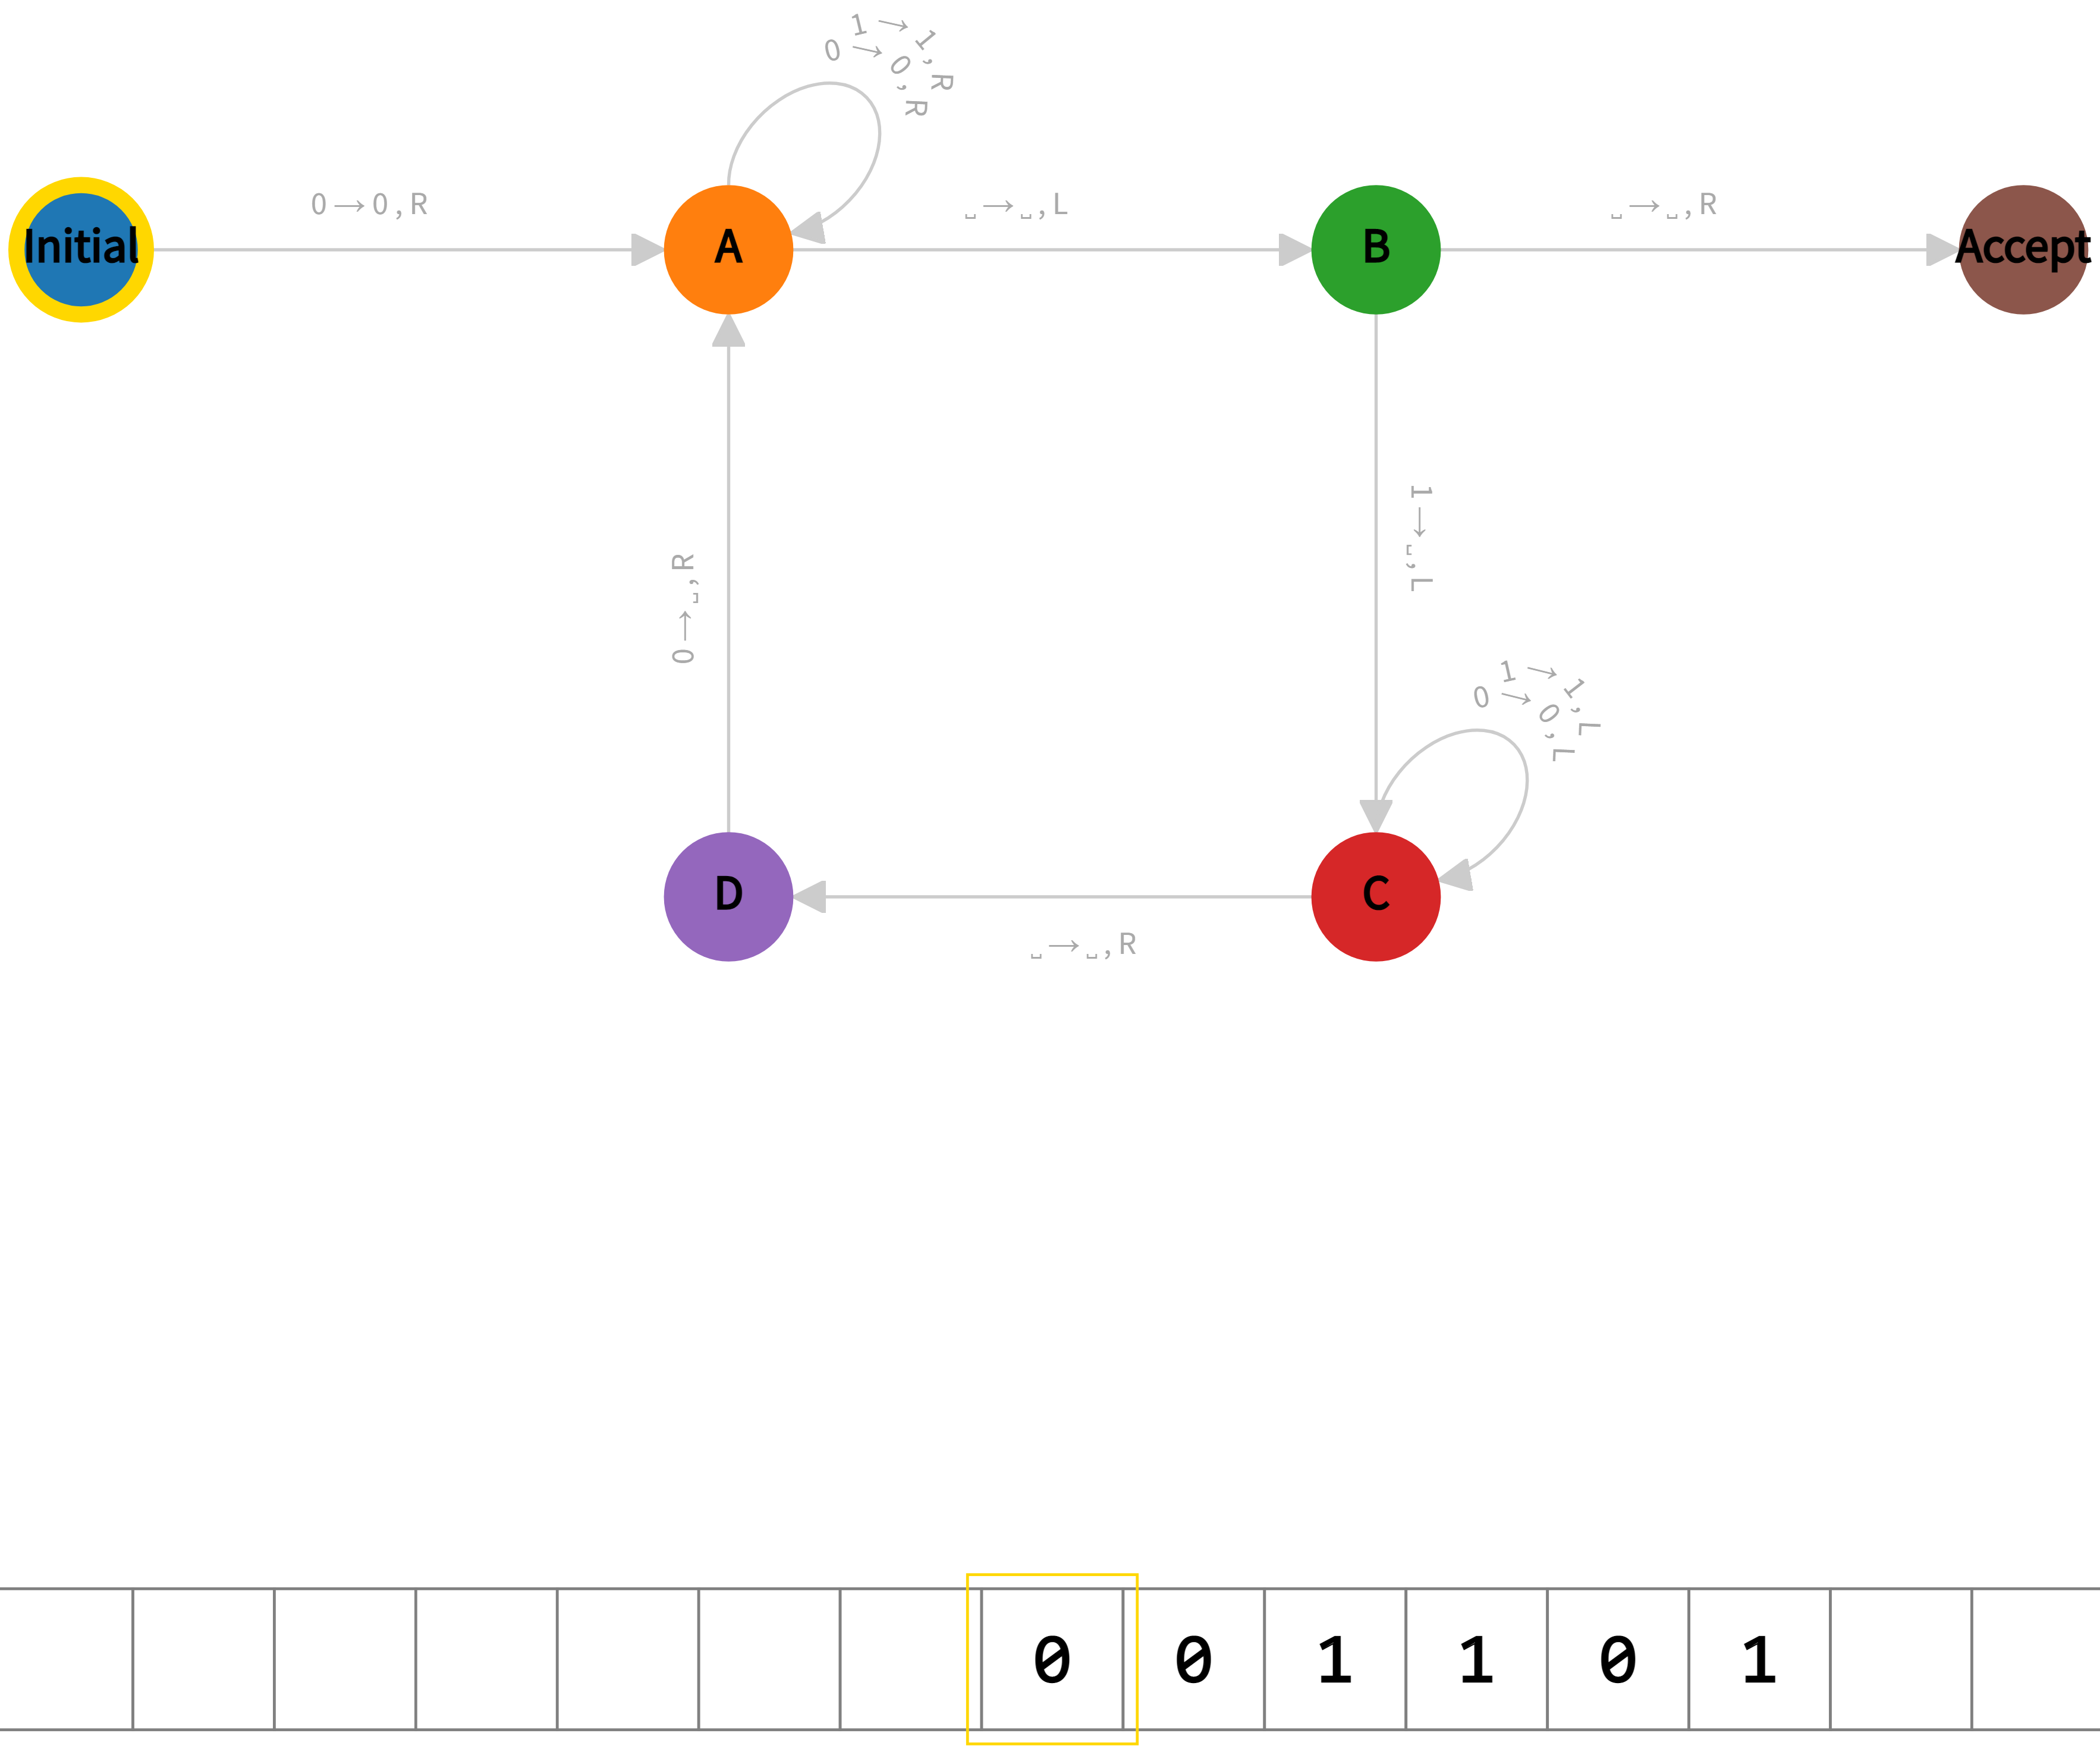
\includegraphics[width=\linewidth]{answers/img/q1-001101-initial.png}
    \caption*{Figure (a): Initial State for $\mathbf{001101}$}
    \label{fig:001101-initial}
  \end{minipage}
  \begin{minipage}{.49\linewidth}
    \centering
    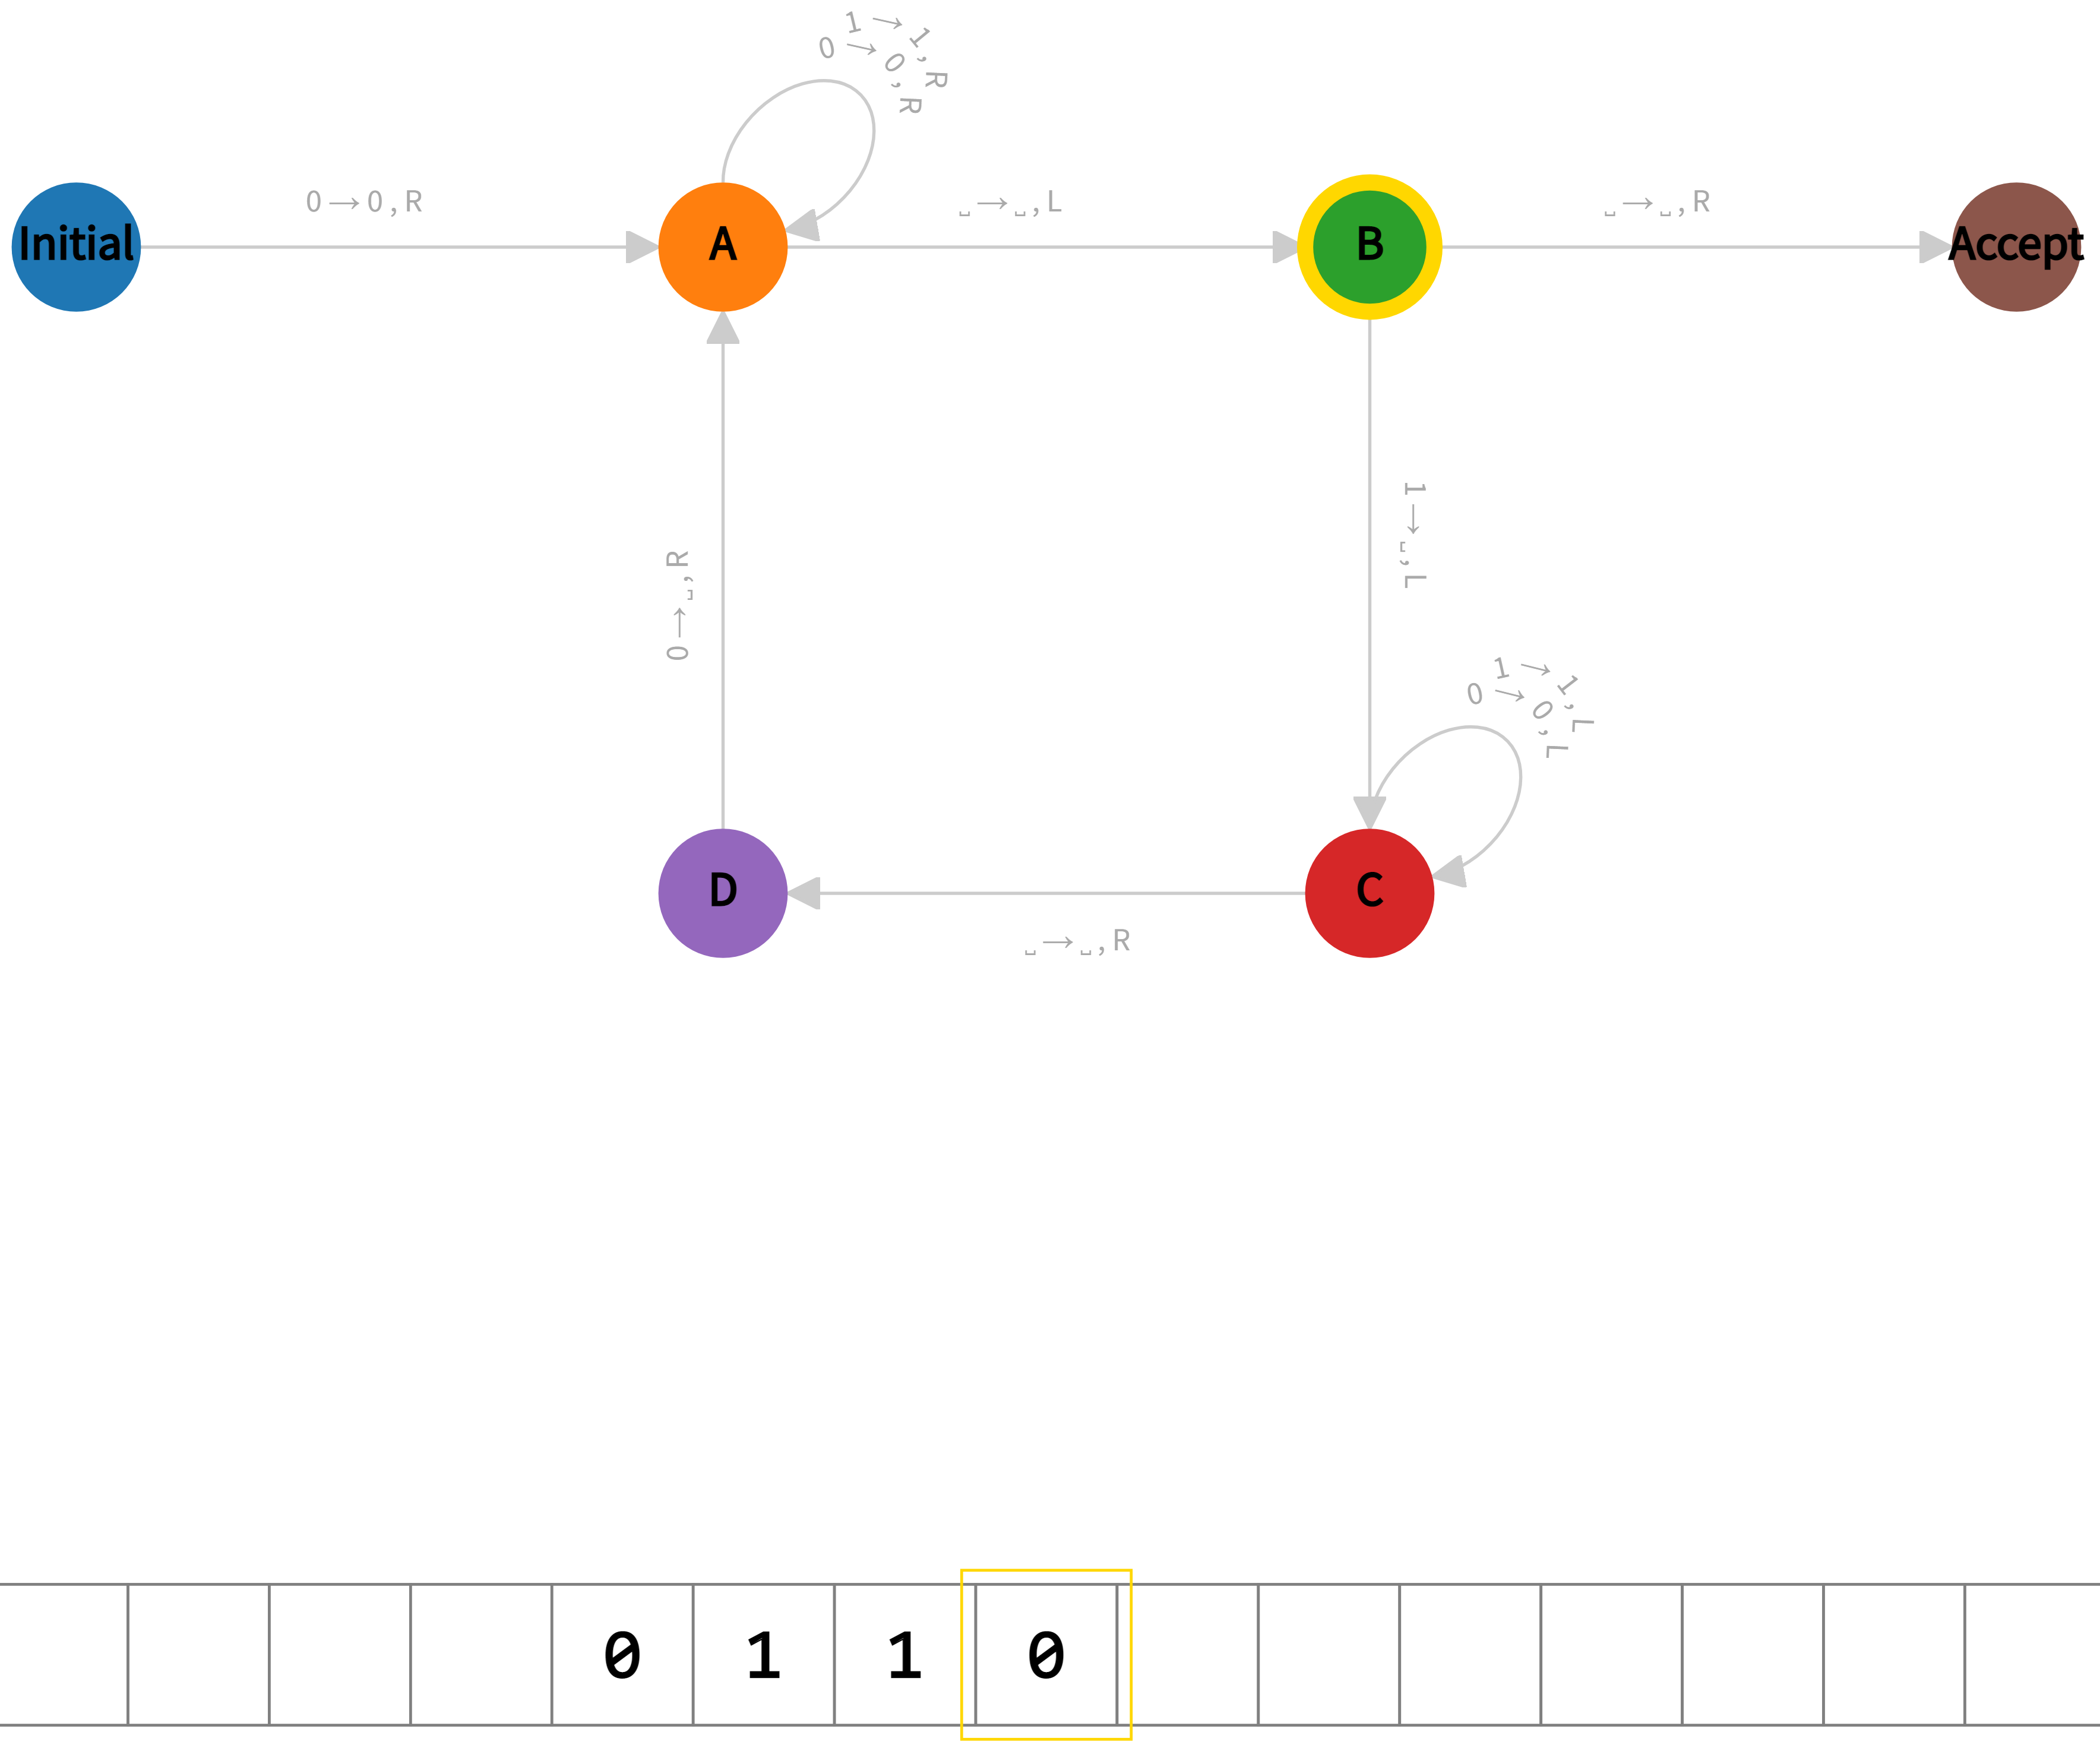
\includegraphics[width=\linewidth]{answers/img/q1-001101-end.png}
    \caption*{Figure (b): End State for $\mathbf{001101}$}
    \label{fig:001101-end}
  \end{minipage}
  \caption{States for $\mathbf{001101}$}
  \label{fig:in-001101}
\end{figure}

\subsubsection*{Input: 100011 $|$ Reject}
\label{q1-100011}

\begin{figure}[ht]
  \centering
  \begin{minipage}{.49\linewidth}
    \centering
    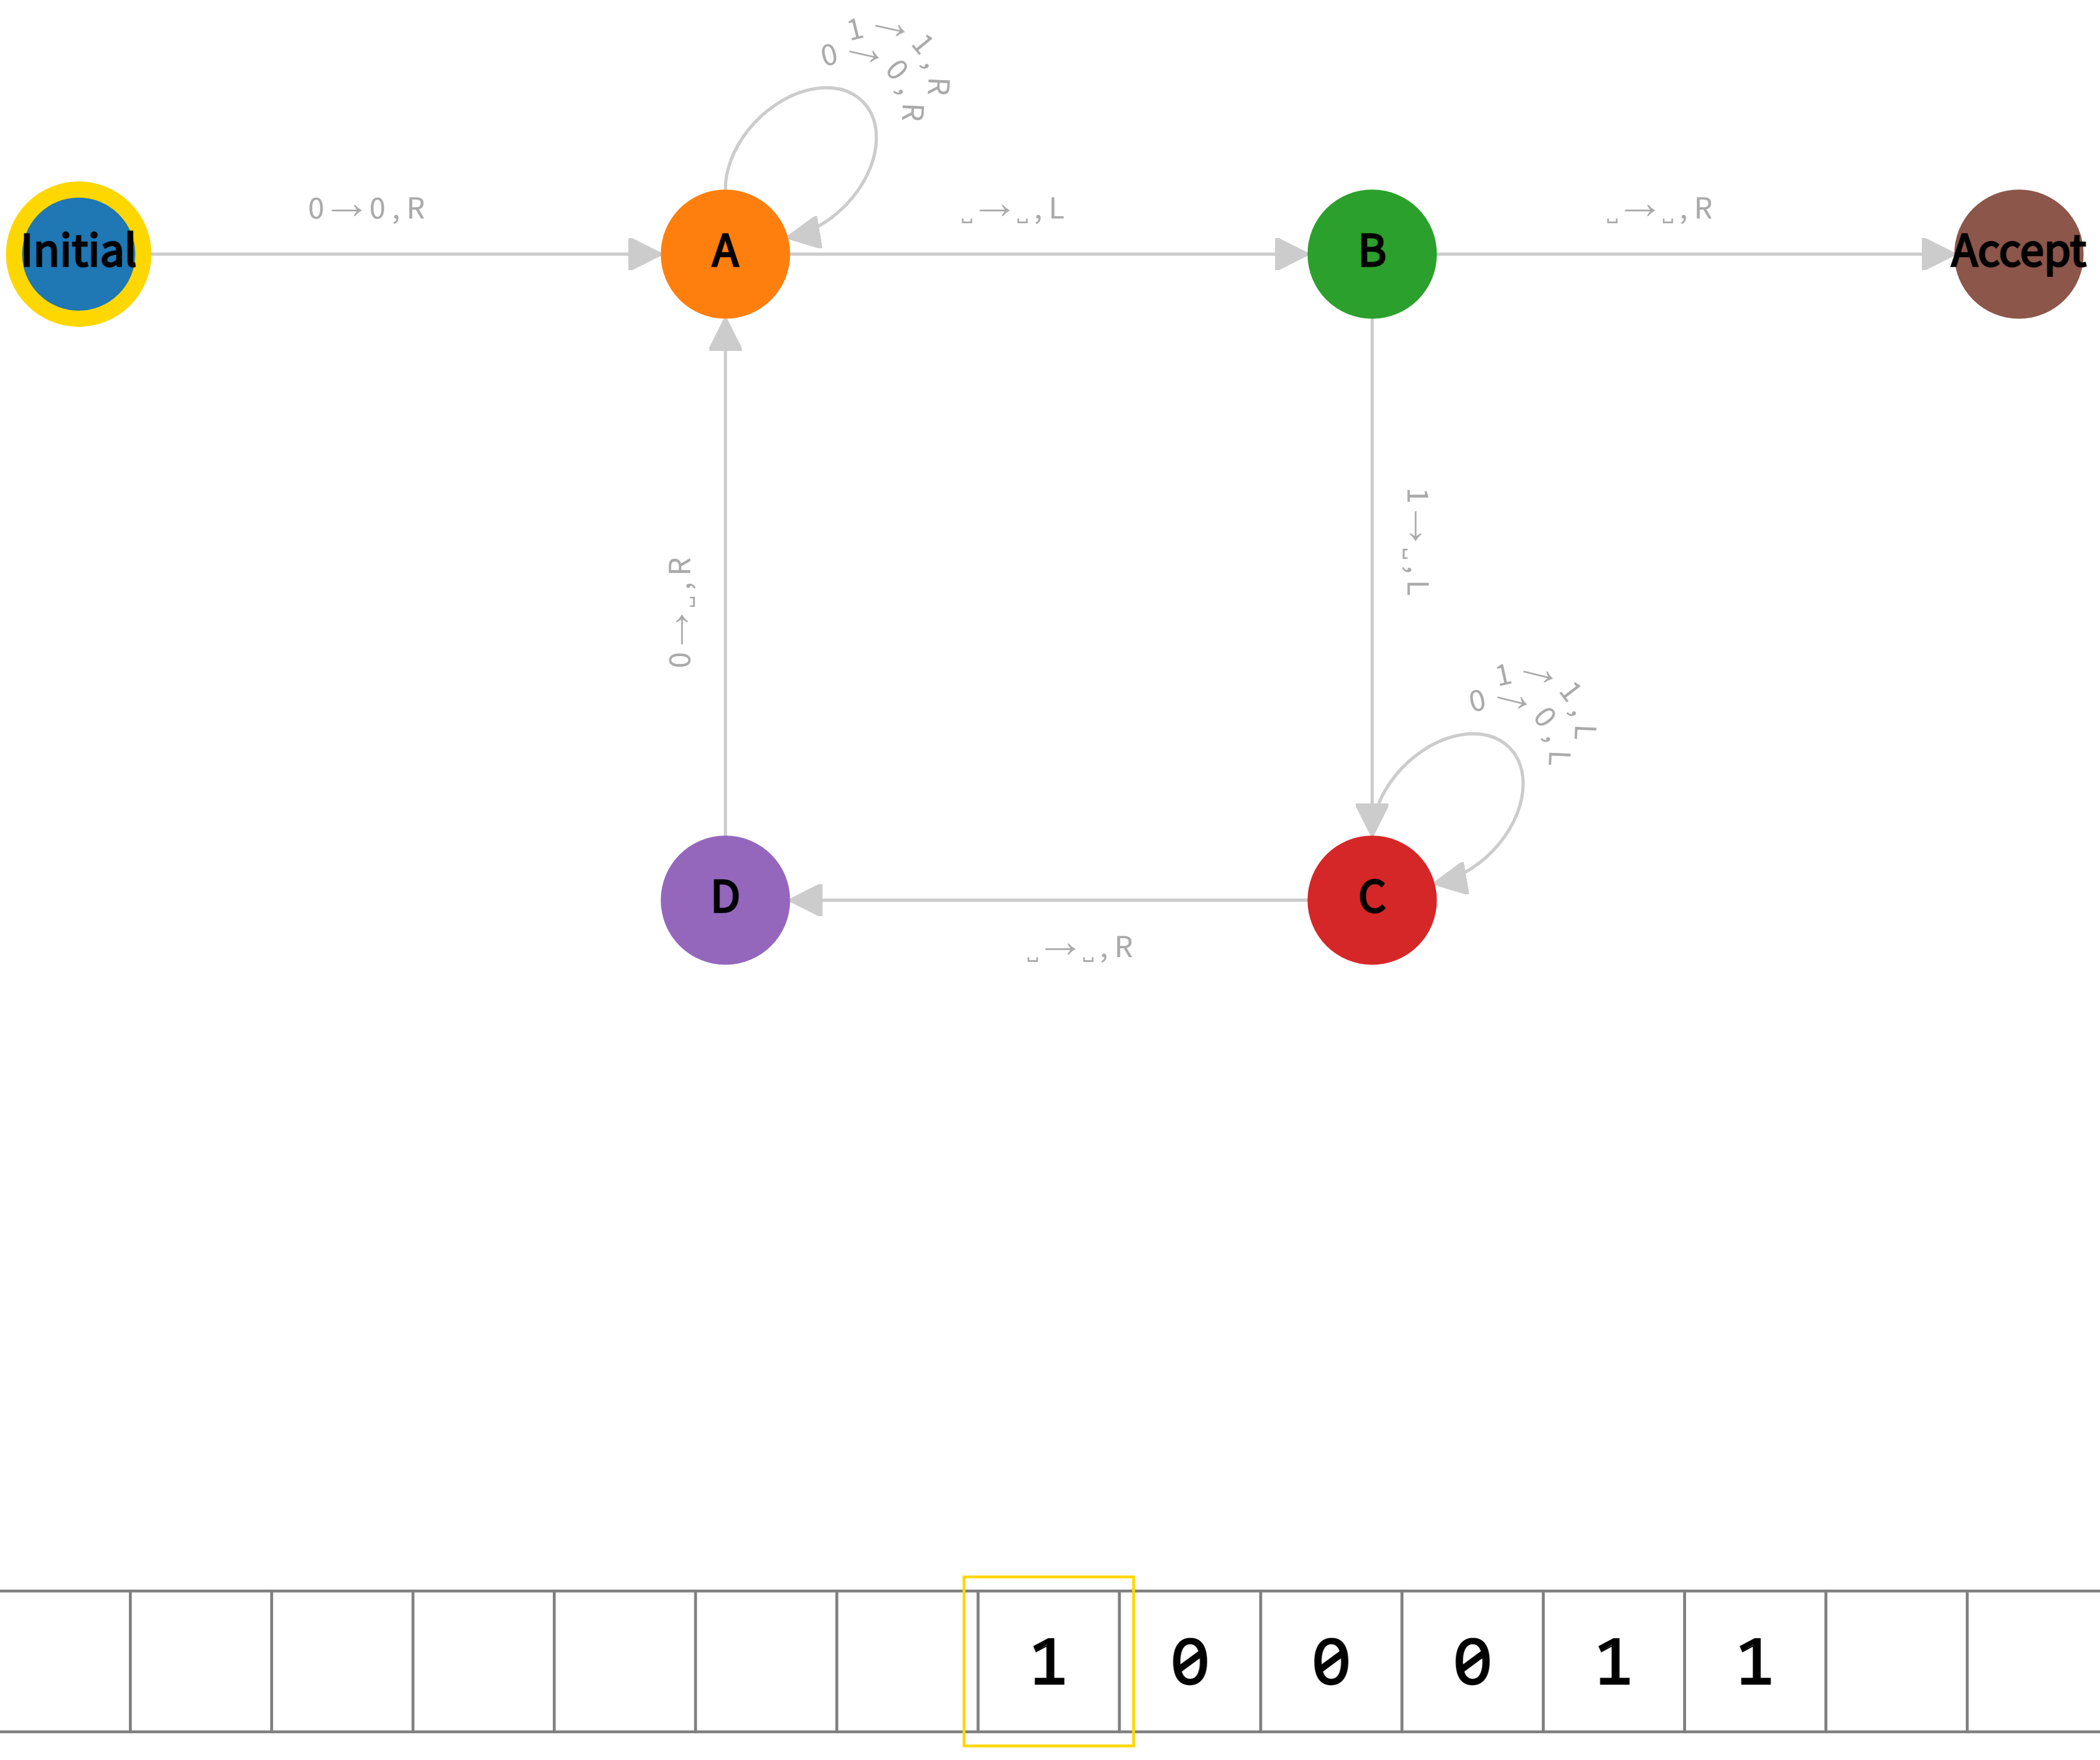
\includegraphics[width=\linewidth]{answers/img/q1-100011-initial.png}
    \caption*{Figure (a): Initial State for $\mathbf{100011}$}
    \label{fig:100011-initial}
  \end{minipage}
  \begin{minipage}{.49\linewidth}
    \centering
    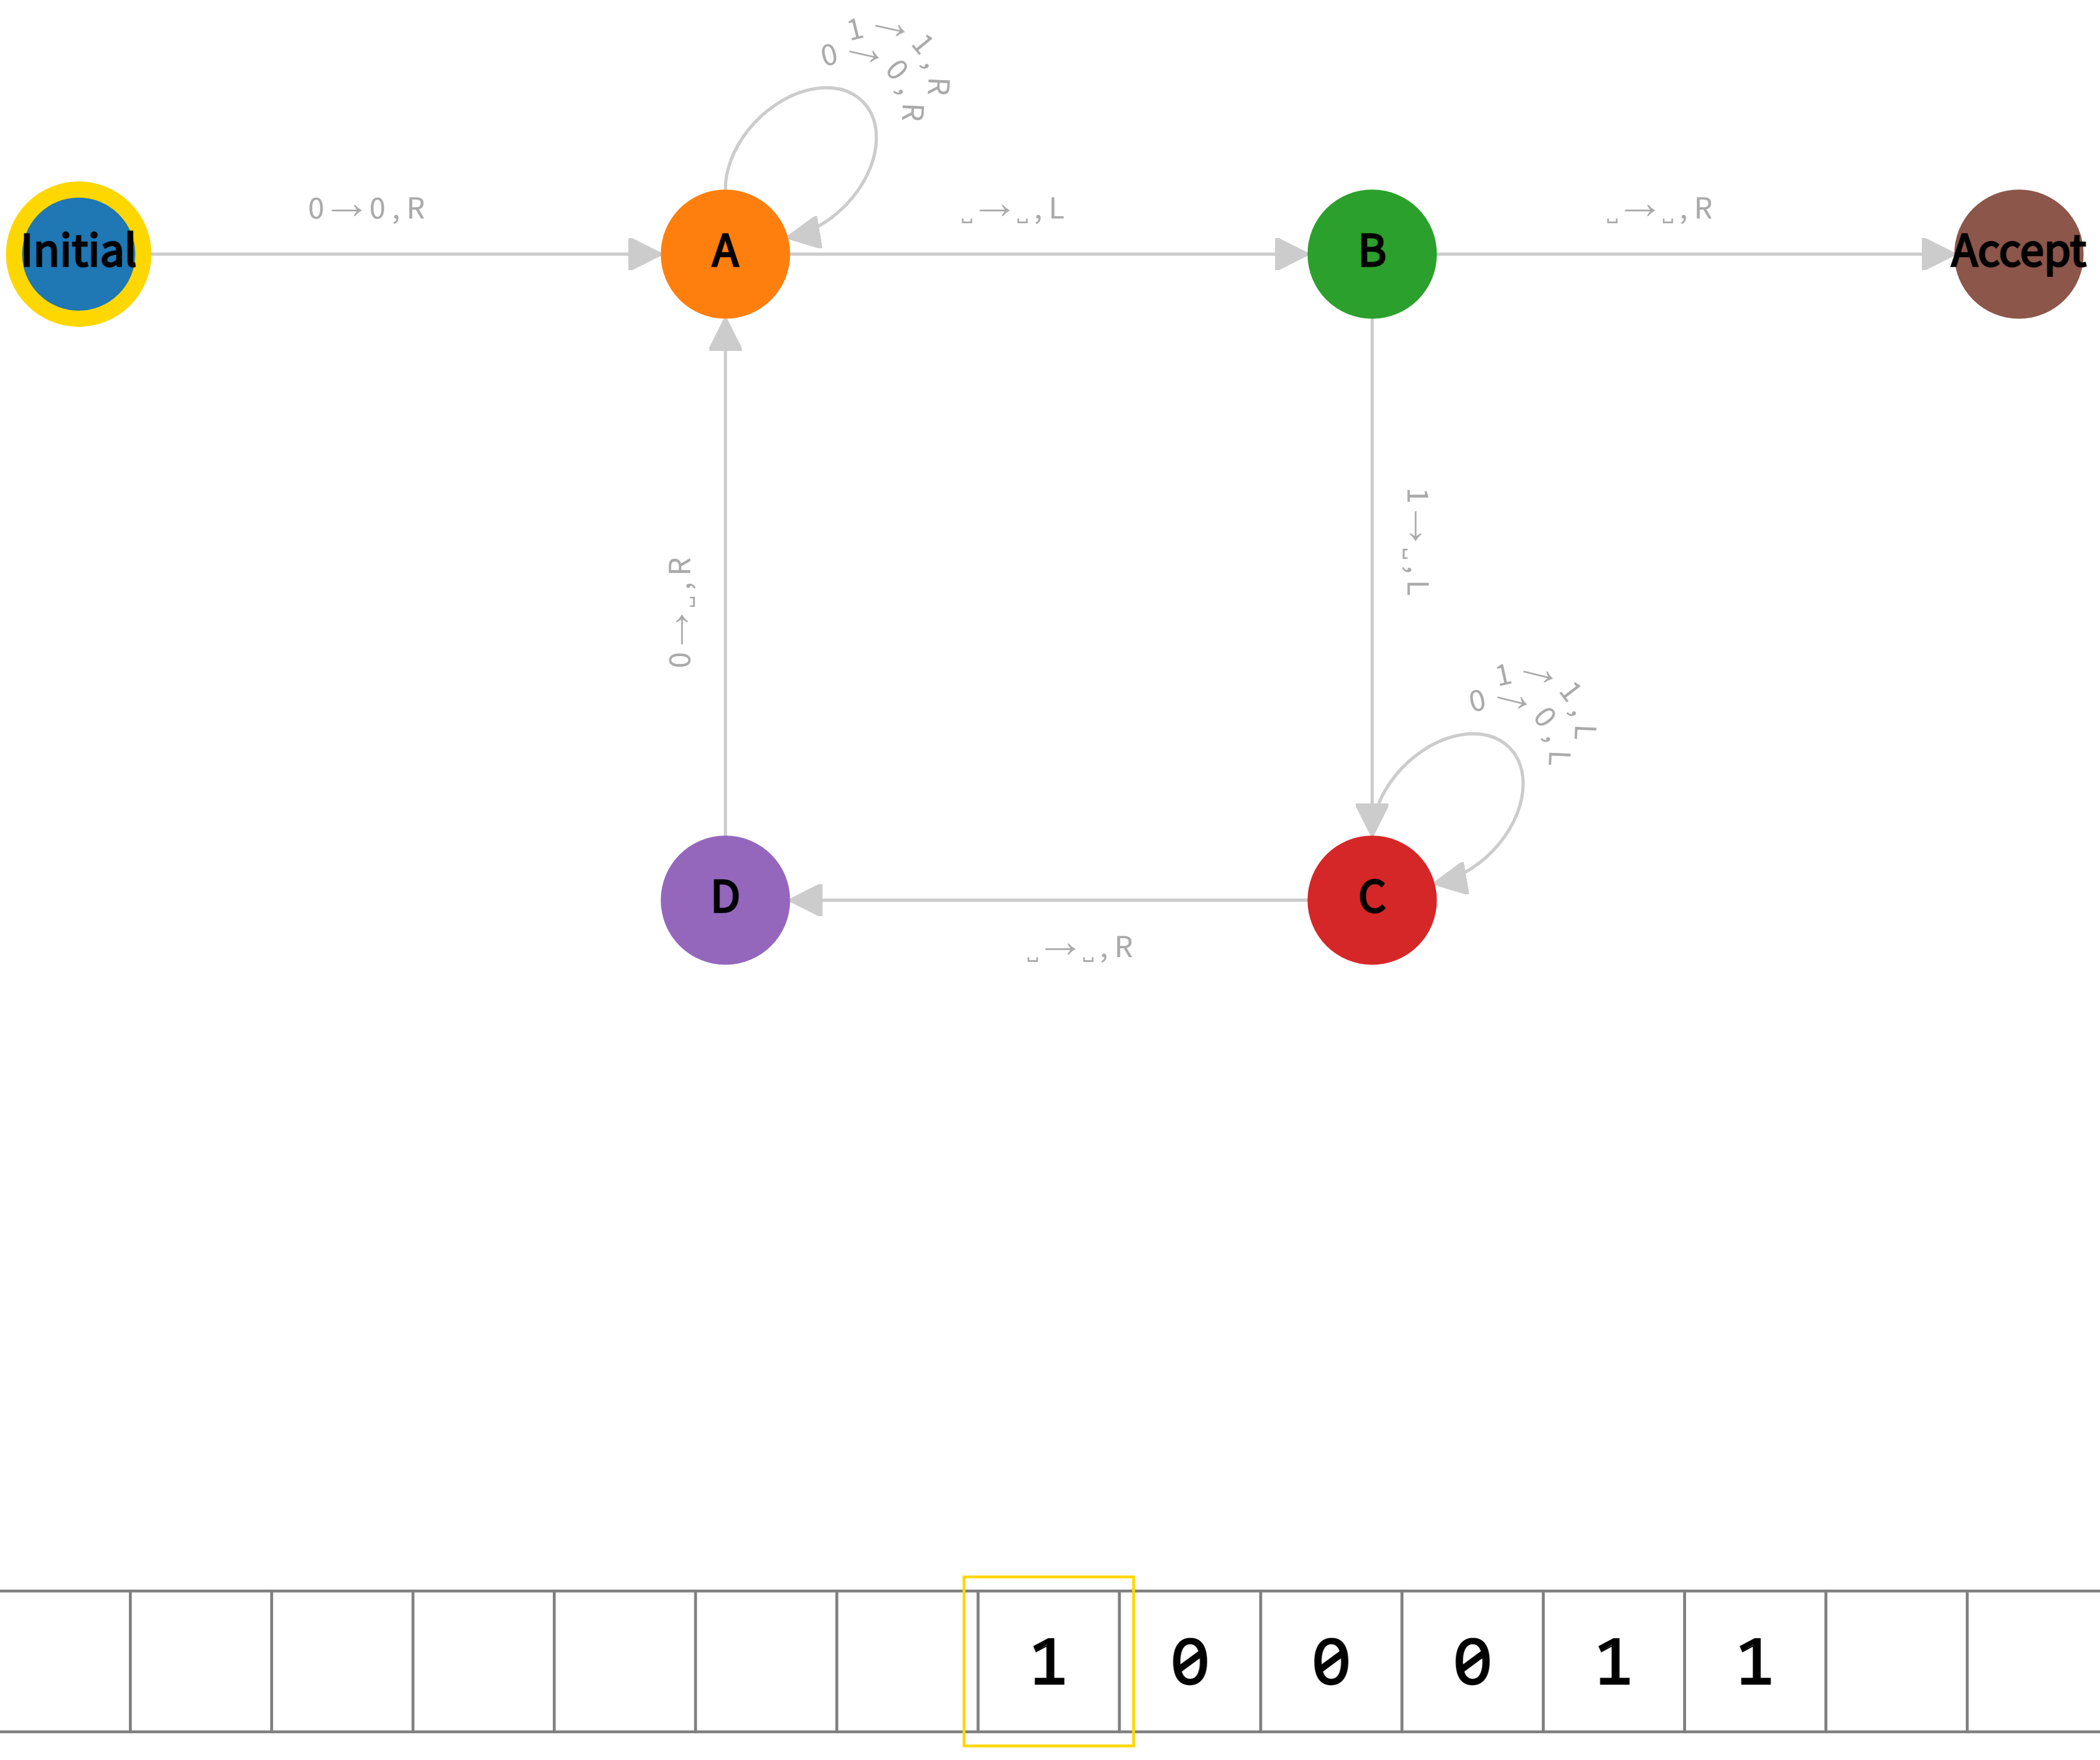
\includegraphics[width=\linewidth]{answers/img/q1-100011-end.png}
    \caption*{Figure (b): End State for $\mathbf{100011}$}
    \label{fig:100011-end}
  \end{minipage}
  \caption{States for $\mathbf{100011}$}
  \label{fig:in-100011}
\end{figure}

\vspace*{\fill}



% --- General Description ---

% Machine will start in the beginning of the string (namely, $0^{th}$ index). Then it will scan to the right for an $\blank$ symbol. 

% When it found the $\blank$ symbol, it will move to the left. 

% If there is a 1, then a $\blank$ will be written and start scanning to the left for another $blank$ symbol.

% If there is a $\blank$, then accepts

% When it found the first $blank$, it will move the right. If there is a 0, then a $\blank$ will be written.


\newpage

\section*{Answer 2}
\label{answer-2}

\vspace*{\fill}
\begin{figure}[h] % SS of TM
  \centering
  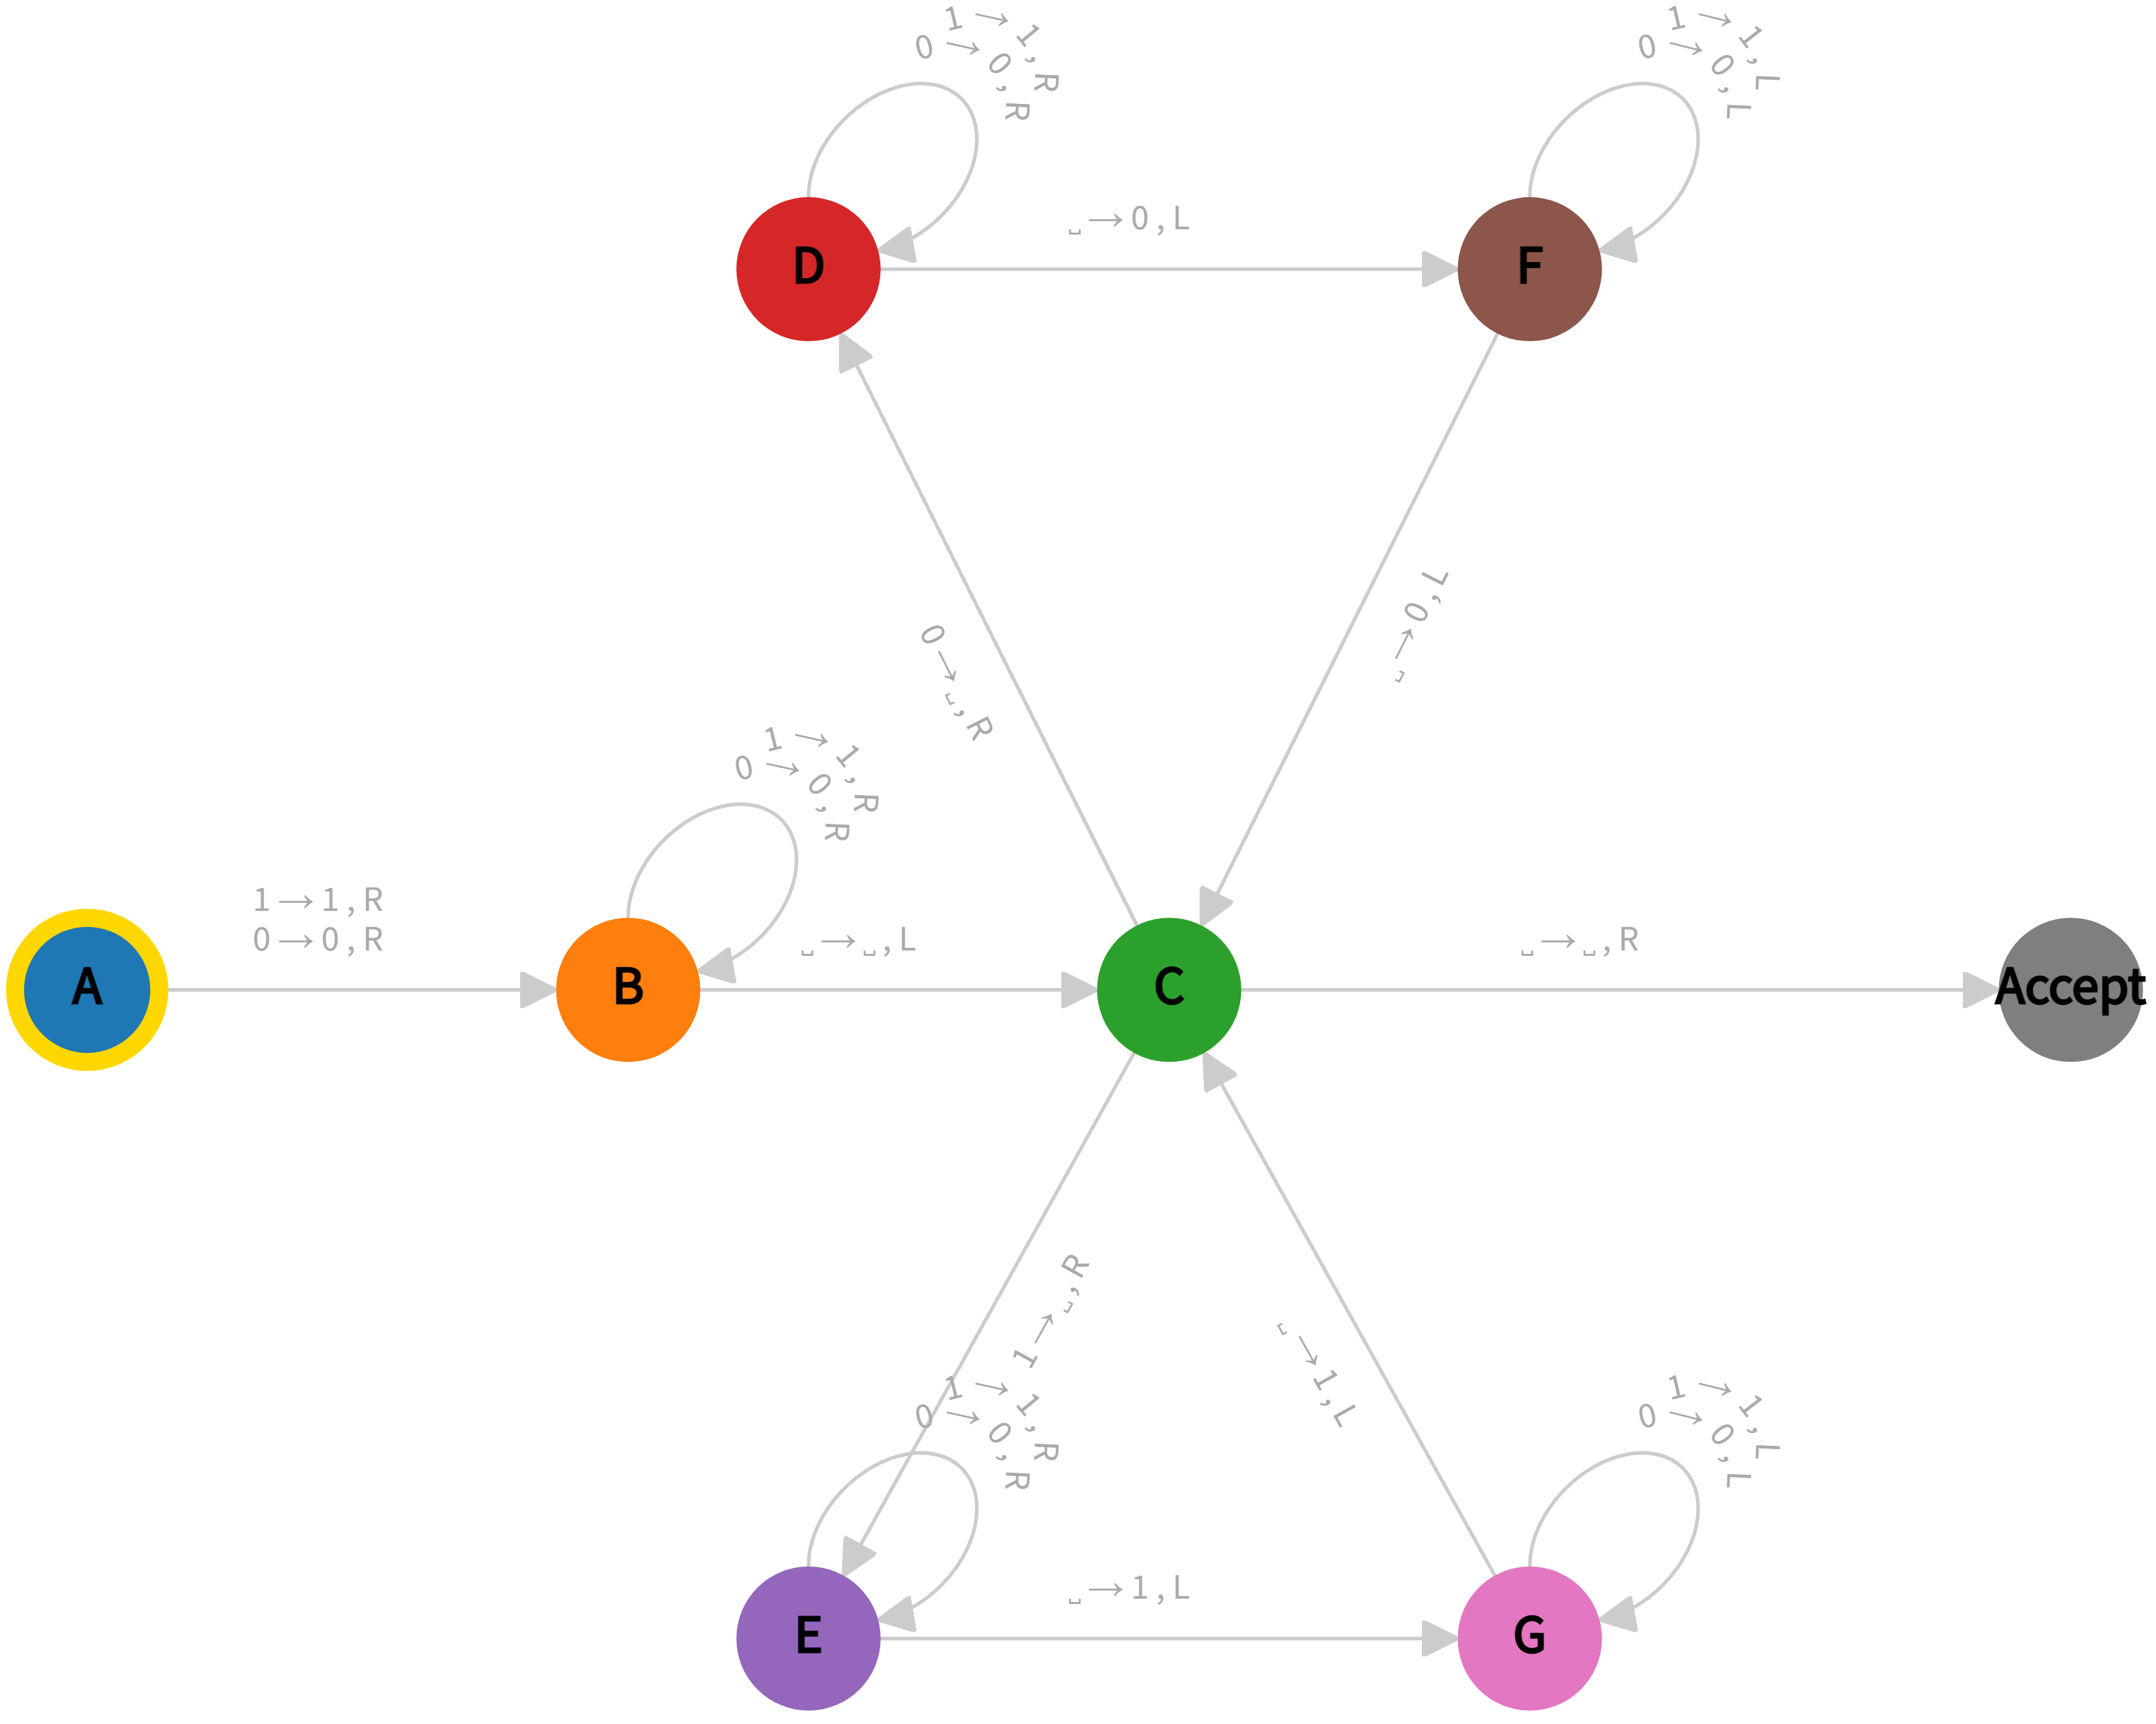
\includegraphics[width=\linewidth]{answers/img/q2-machine.png}
  \caption{\textit{Screenshot of the Turing Machine designed for Q2}}
  \label{fig:q2-machine}
\end{figure}
\vspace*{\fill}

\newpage

\begin{center} \subsection*{Descriptions of States} \end{center}
\label{q2:description-of-states}

\subsubsection*{State: A}
\label{q2-state:initial}

\textit{It is the start state}. If string starts with $\blank$, machine immediately stops in this state. If string starts with $\mathbf{0}$ or $\mathbf{0}$, head is moved to right and state of machine goes to state \hyperref[q2-state:B]{$\mathbf{B}$}.

\subsubsection*{State: B}
\label{q2-state:B}

It scans to the right for the first $\blank$. When $\blank$ is found, head is moved to left and state of machine goes to state \hyperref[q2-state:C]{$\mathbf{C}$}. 

It is used only once to find the last symbol in the string.

\subsubsection*{State: C}
\label{q2-state:C}

It is the state indicating that the symbol below the head needs to be put the end of string; that is, head is on the symbol that will be copied to the end of the string if state of machine is in state \hyperref[q2-state:C]{$\mathbf{C}$}. In this state,
\begin{itemize}
  \item If $\mathbf{0}$ is read, a $\blank$ is temporarily placed and head is moved right and state of machine goes to state \hyperref[q2-state:D]{$\mathbf{D}$} (The upper part of states, as shown in \hyperref[fig:q2-machine]{Figure 8}. This part remembers the symbol was $\mathbf{0}$).
  \item If $\mathbf{1}$ is read, a $\blank$ is temporarily placed and head is moved right and state of machine goes to state \hyperref[q2-state:E]{$\mathbf{E}$} (The lower part of states, as shown in \hyperref[fig:q2-machine]{Figure 8}. This part remembers the symbol was $\mathbf{1}$).
  \item If $\blank$ is read, it means that computing is done without any error or crash. State of the machine goes to state \hyperref[q2-state:Accept]{$\mathbf{Accept}$}
\end{itemize}

\subsubsection*{State: D}
\label{q2-state:D}

It scans to the right for the first $\blank$. The important part is that it knows (symbol that will be copied was $\mathbf{0}$) symbol will be written is $\mathbf{0}$. When $\blank$ is found,
\begin{itemize}
  \item $\mathbf{0}$ is placed,
  \item head is moved left, and
  \item state of the machine goes to state \hyperref[q2-state:F]{$\mathbf{F}$}.
\end{itemize}

\subsubsection*{State: F}
\label{q2-state:F}

It scans to the left for the $\blank$ that is placed temporarily. The important part is that it knows (copied symbol was $\mathbf{0}$) symbol will be written is $\mathbf{0}$. When $\blank$ is found,
\begin{itemize}
  \item $\mathbf{0}$ is reinserted to its old place,
  \item head is moved left (next is symbol that will be copied or a $\blank$), and
  \item state of the machine goes to state \hyperref[q2-state:C]{$\mathbf{C}$}.
\end{itemize}

\subsubsection*{State: E}
\label{q2-state:E}

It scans to the right for the first $\blank$. The important part is that it knows (symbol that will be copied was $\mathbf{1}$) symbol will be written is $\mathbf{1}$. When $\blank$ is found,
\begin{itemize}
  \item $\mathbf{1}$ is placed,
  \item head is moved left, and
  \item state of the machine goes to state \hyperref[q2-state:G]{$\mathbf{G}$}.
\end{itemize}

\subsubsection*{State: G}
\label{q2-state:G}

It scans to the left for the $\blank$ that is placed temporarily. The important part is that it knows (copied symbol was $\mathbf{1}$) symbol will be written is $\mathbf{1}$. When $\blank$ is found,
\begin{itemize}
  \item $\mathbf{1}$ is reinserted to its old place,
  \item head is moved left (next is symbol that will be copied or a $\blank$), and
  \item state of the machine goes to state \hyperref[q2-state:C]{$\mathbf{C}$}.
\end{itemize}

\subsubsection*{State: Accept}
\label{q2-state:Accept}

\textit{It is state indicating that computing is done without any error or crash}. Therefore, the machine stops, successfully.


\newpage

\begin{center} \subsection*{Input Samples} \end{center}
\label{q2:input-samples}
\vspace*{\fill}

\subsubsection*{Input: 1011}
\label{q2-1011}

\begin{figure}[ht]
  \centering
  \begin{minipage}{.49\linewidth}
    \centering
    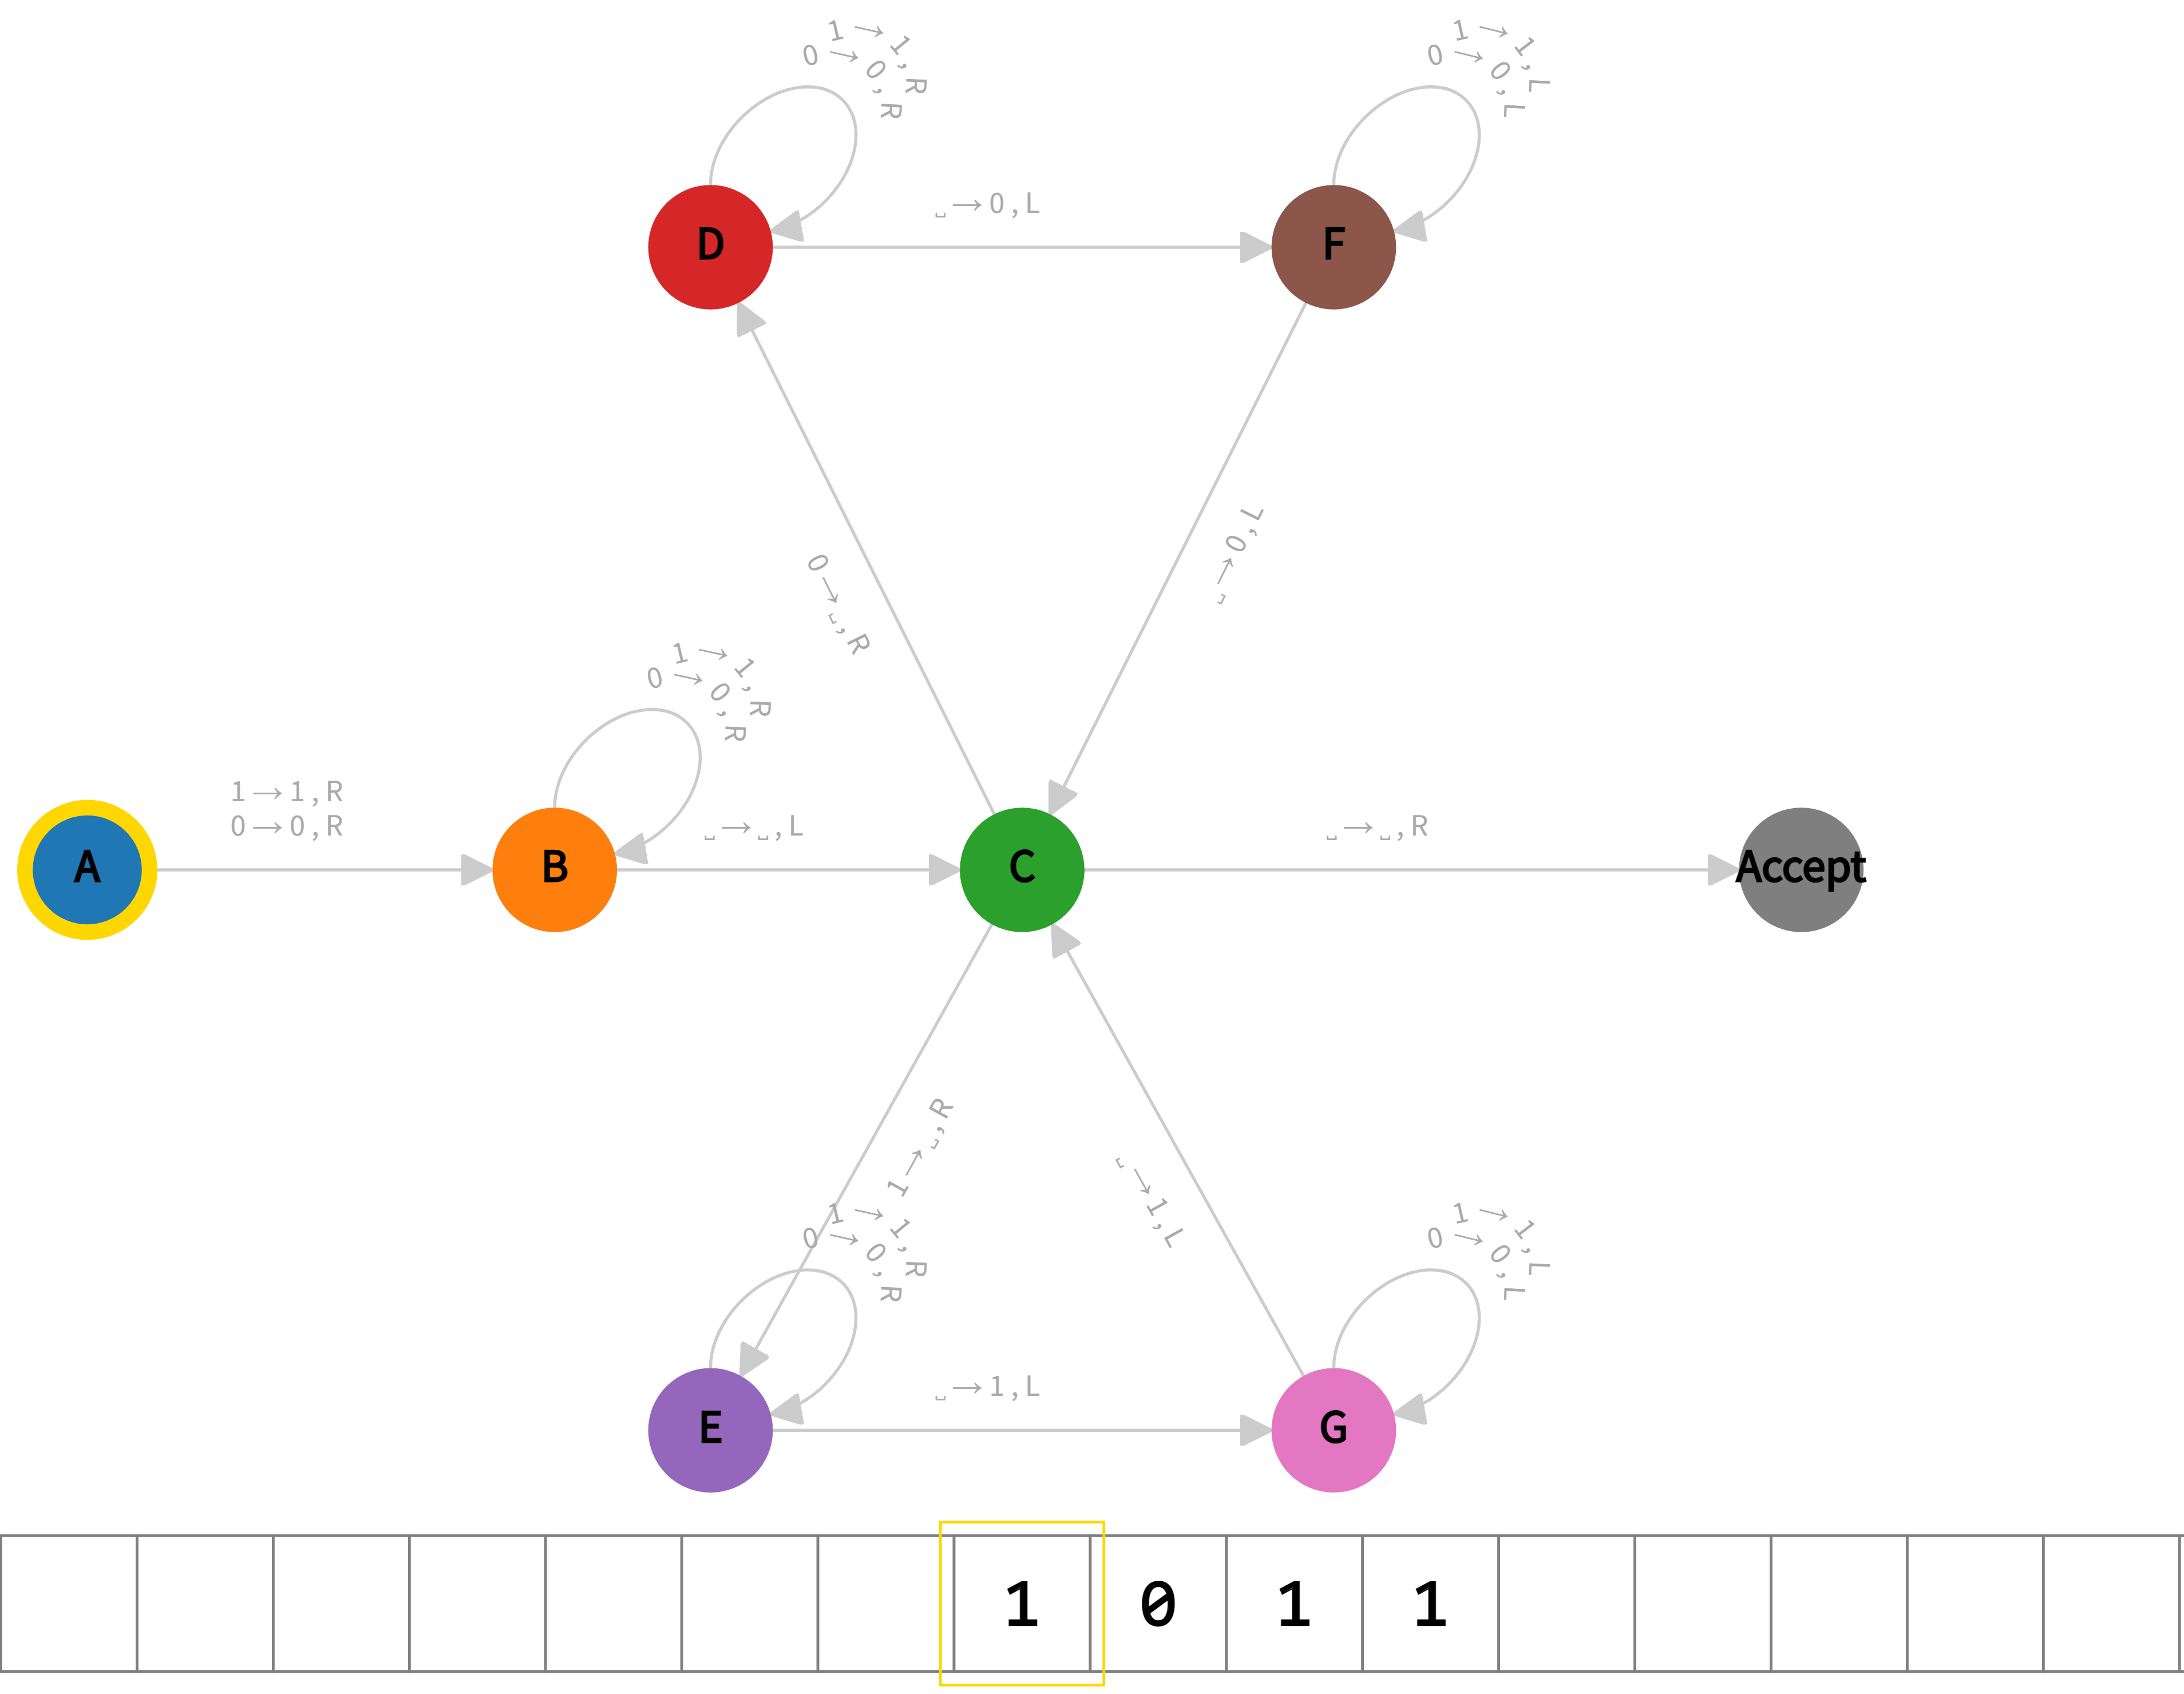
\includegraphics[width=\linewidth]{answers/img/q2-1011-initial.png}
    \caption*{Figure (a): Initial State for $\mathbf{1011}$}
    \label{fig:1011-initial}
  \end{minipage}
  \begin{minipage}{.49\linewidth}
    \centering
    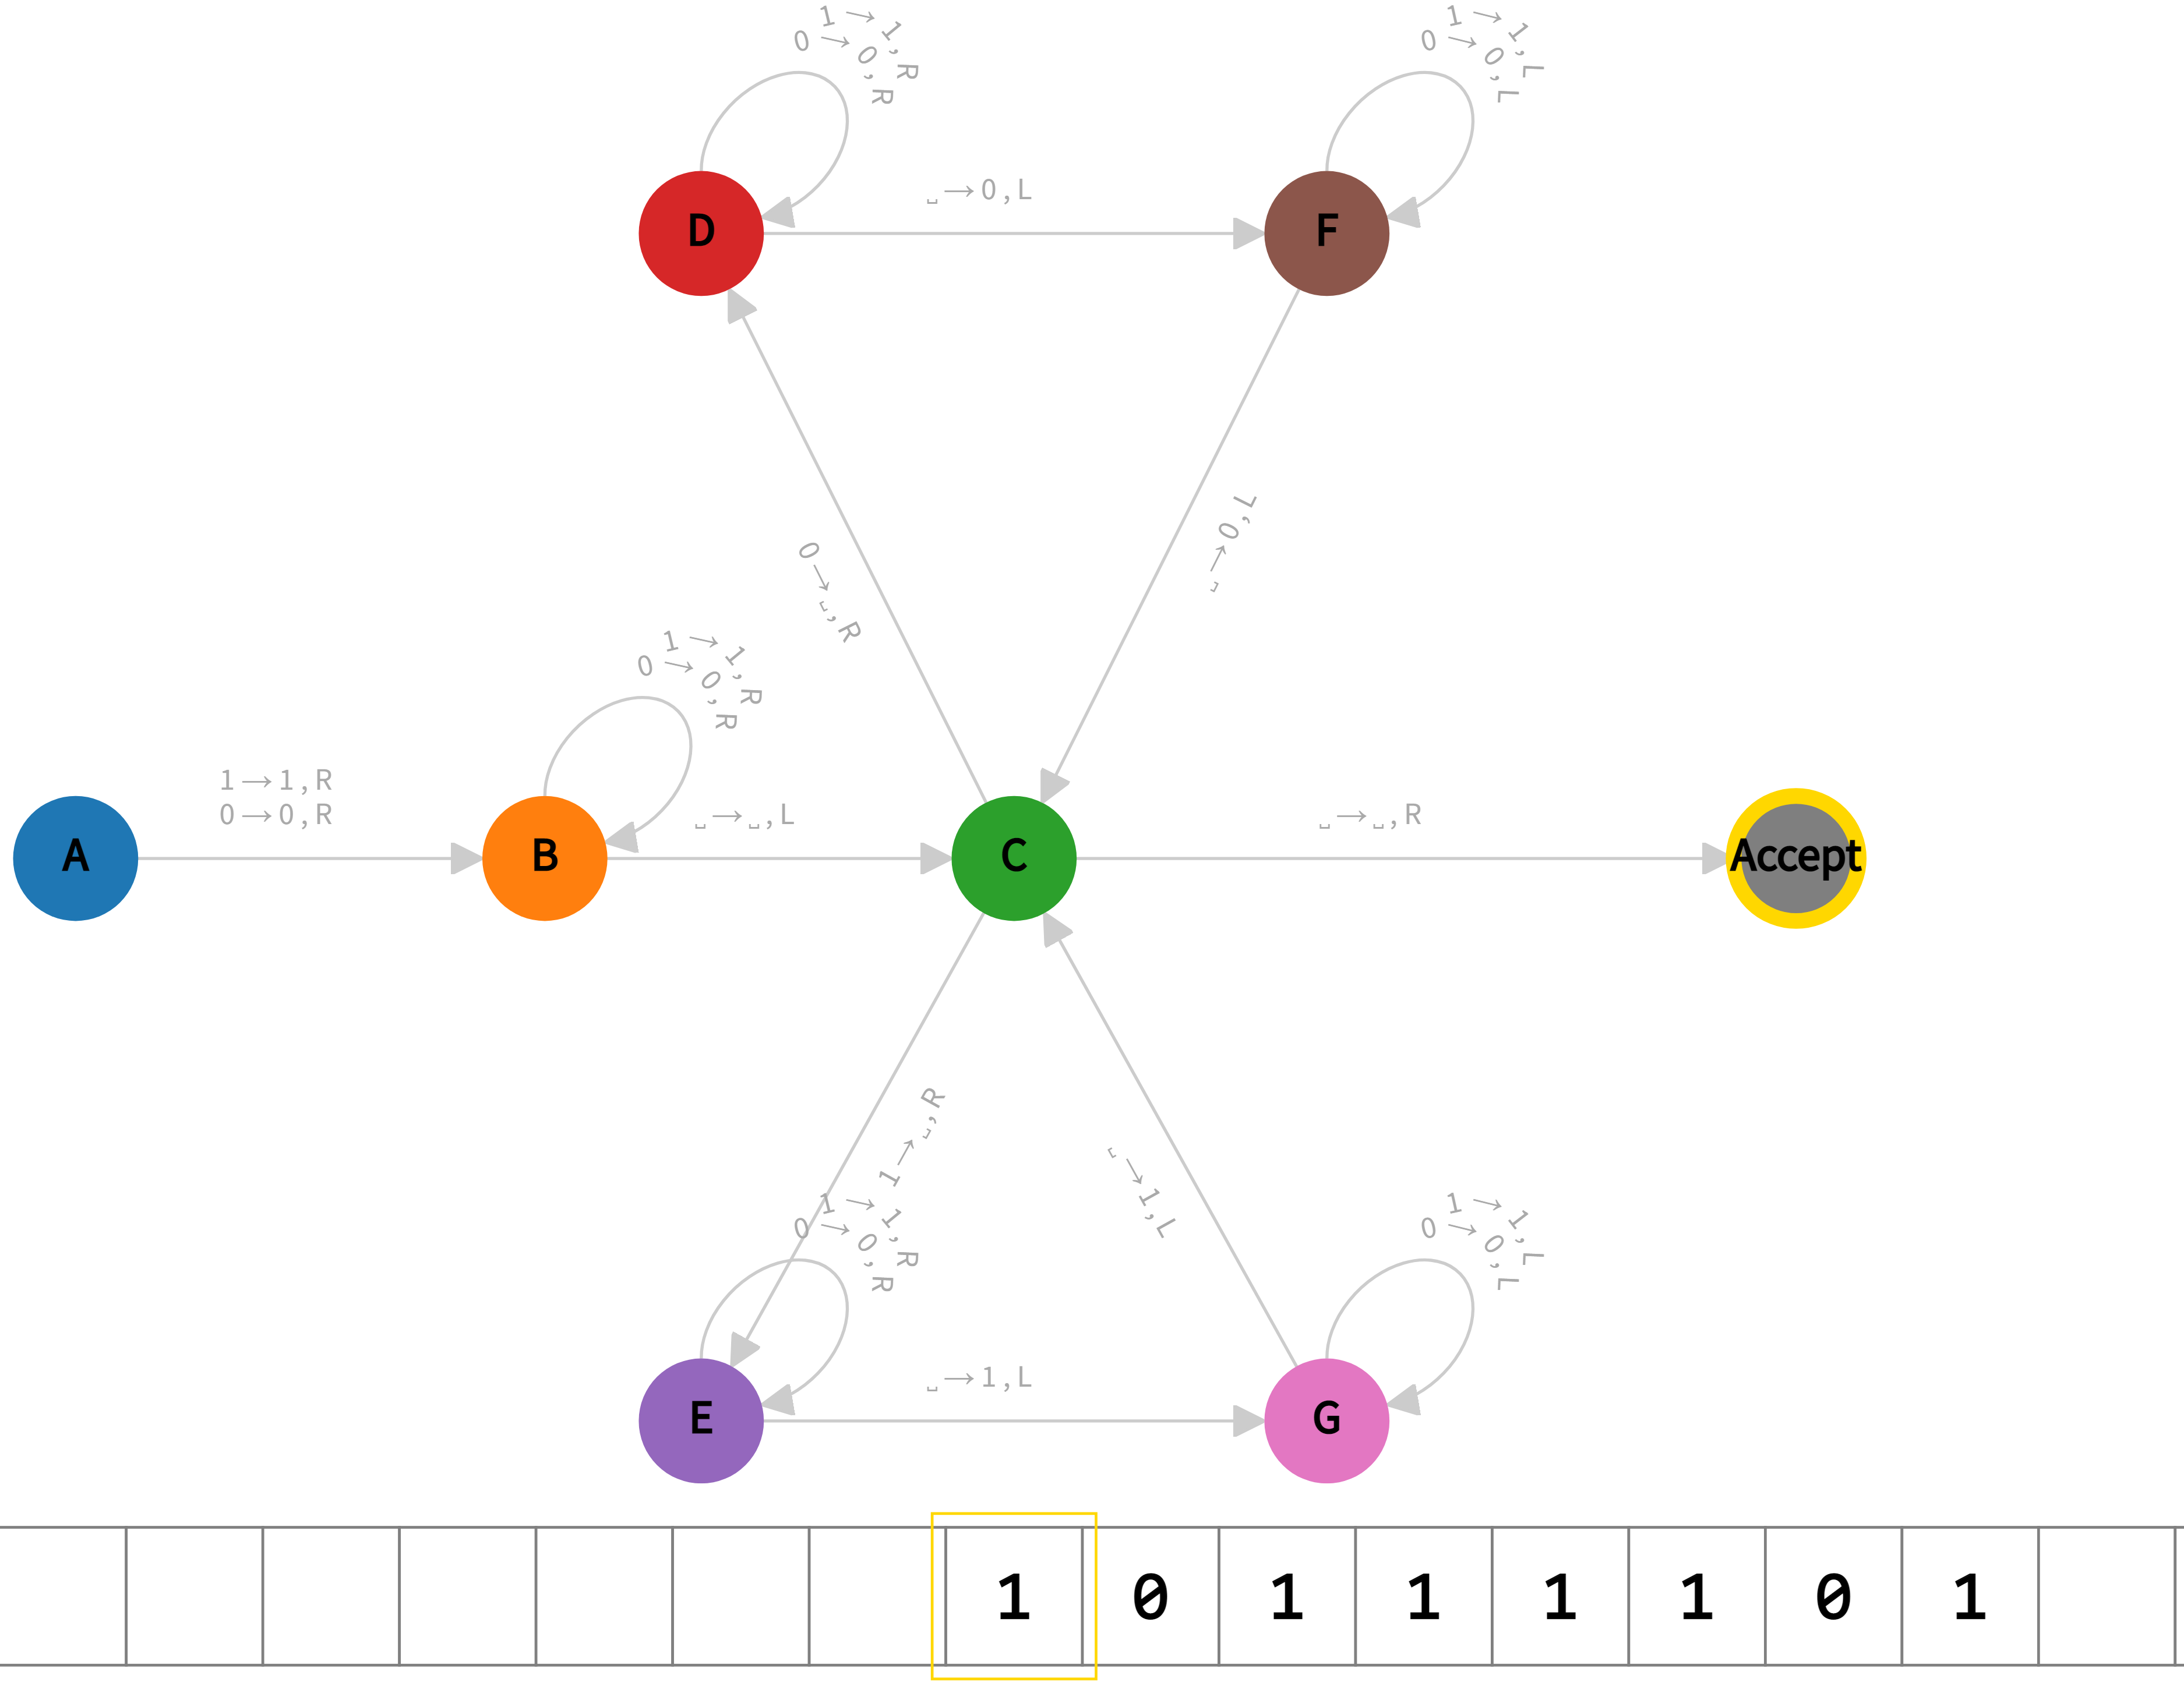
\includegraphics[width=\linewidth]{answers/img/q2-1011-end.png}
    \caption*{Figure (b): End State for $\mathbf{1011}$}
    \label{fig:1011-end}
  \end{minipage}
  \caption{States for $\mathbf{1011}$}
  \label{fig:in-1011}
\end{figure}

\subsubsection*{Input: 1110}
\label{q2-1110}

\begin{figure}[ht]
  \centering
  \begin{minipage}{.49\linewidth}
    \centering
    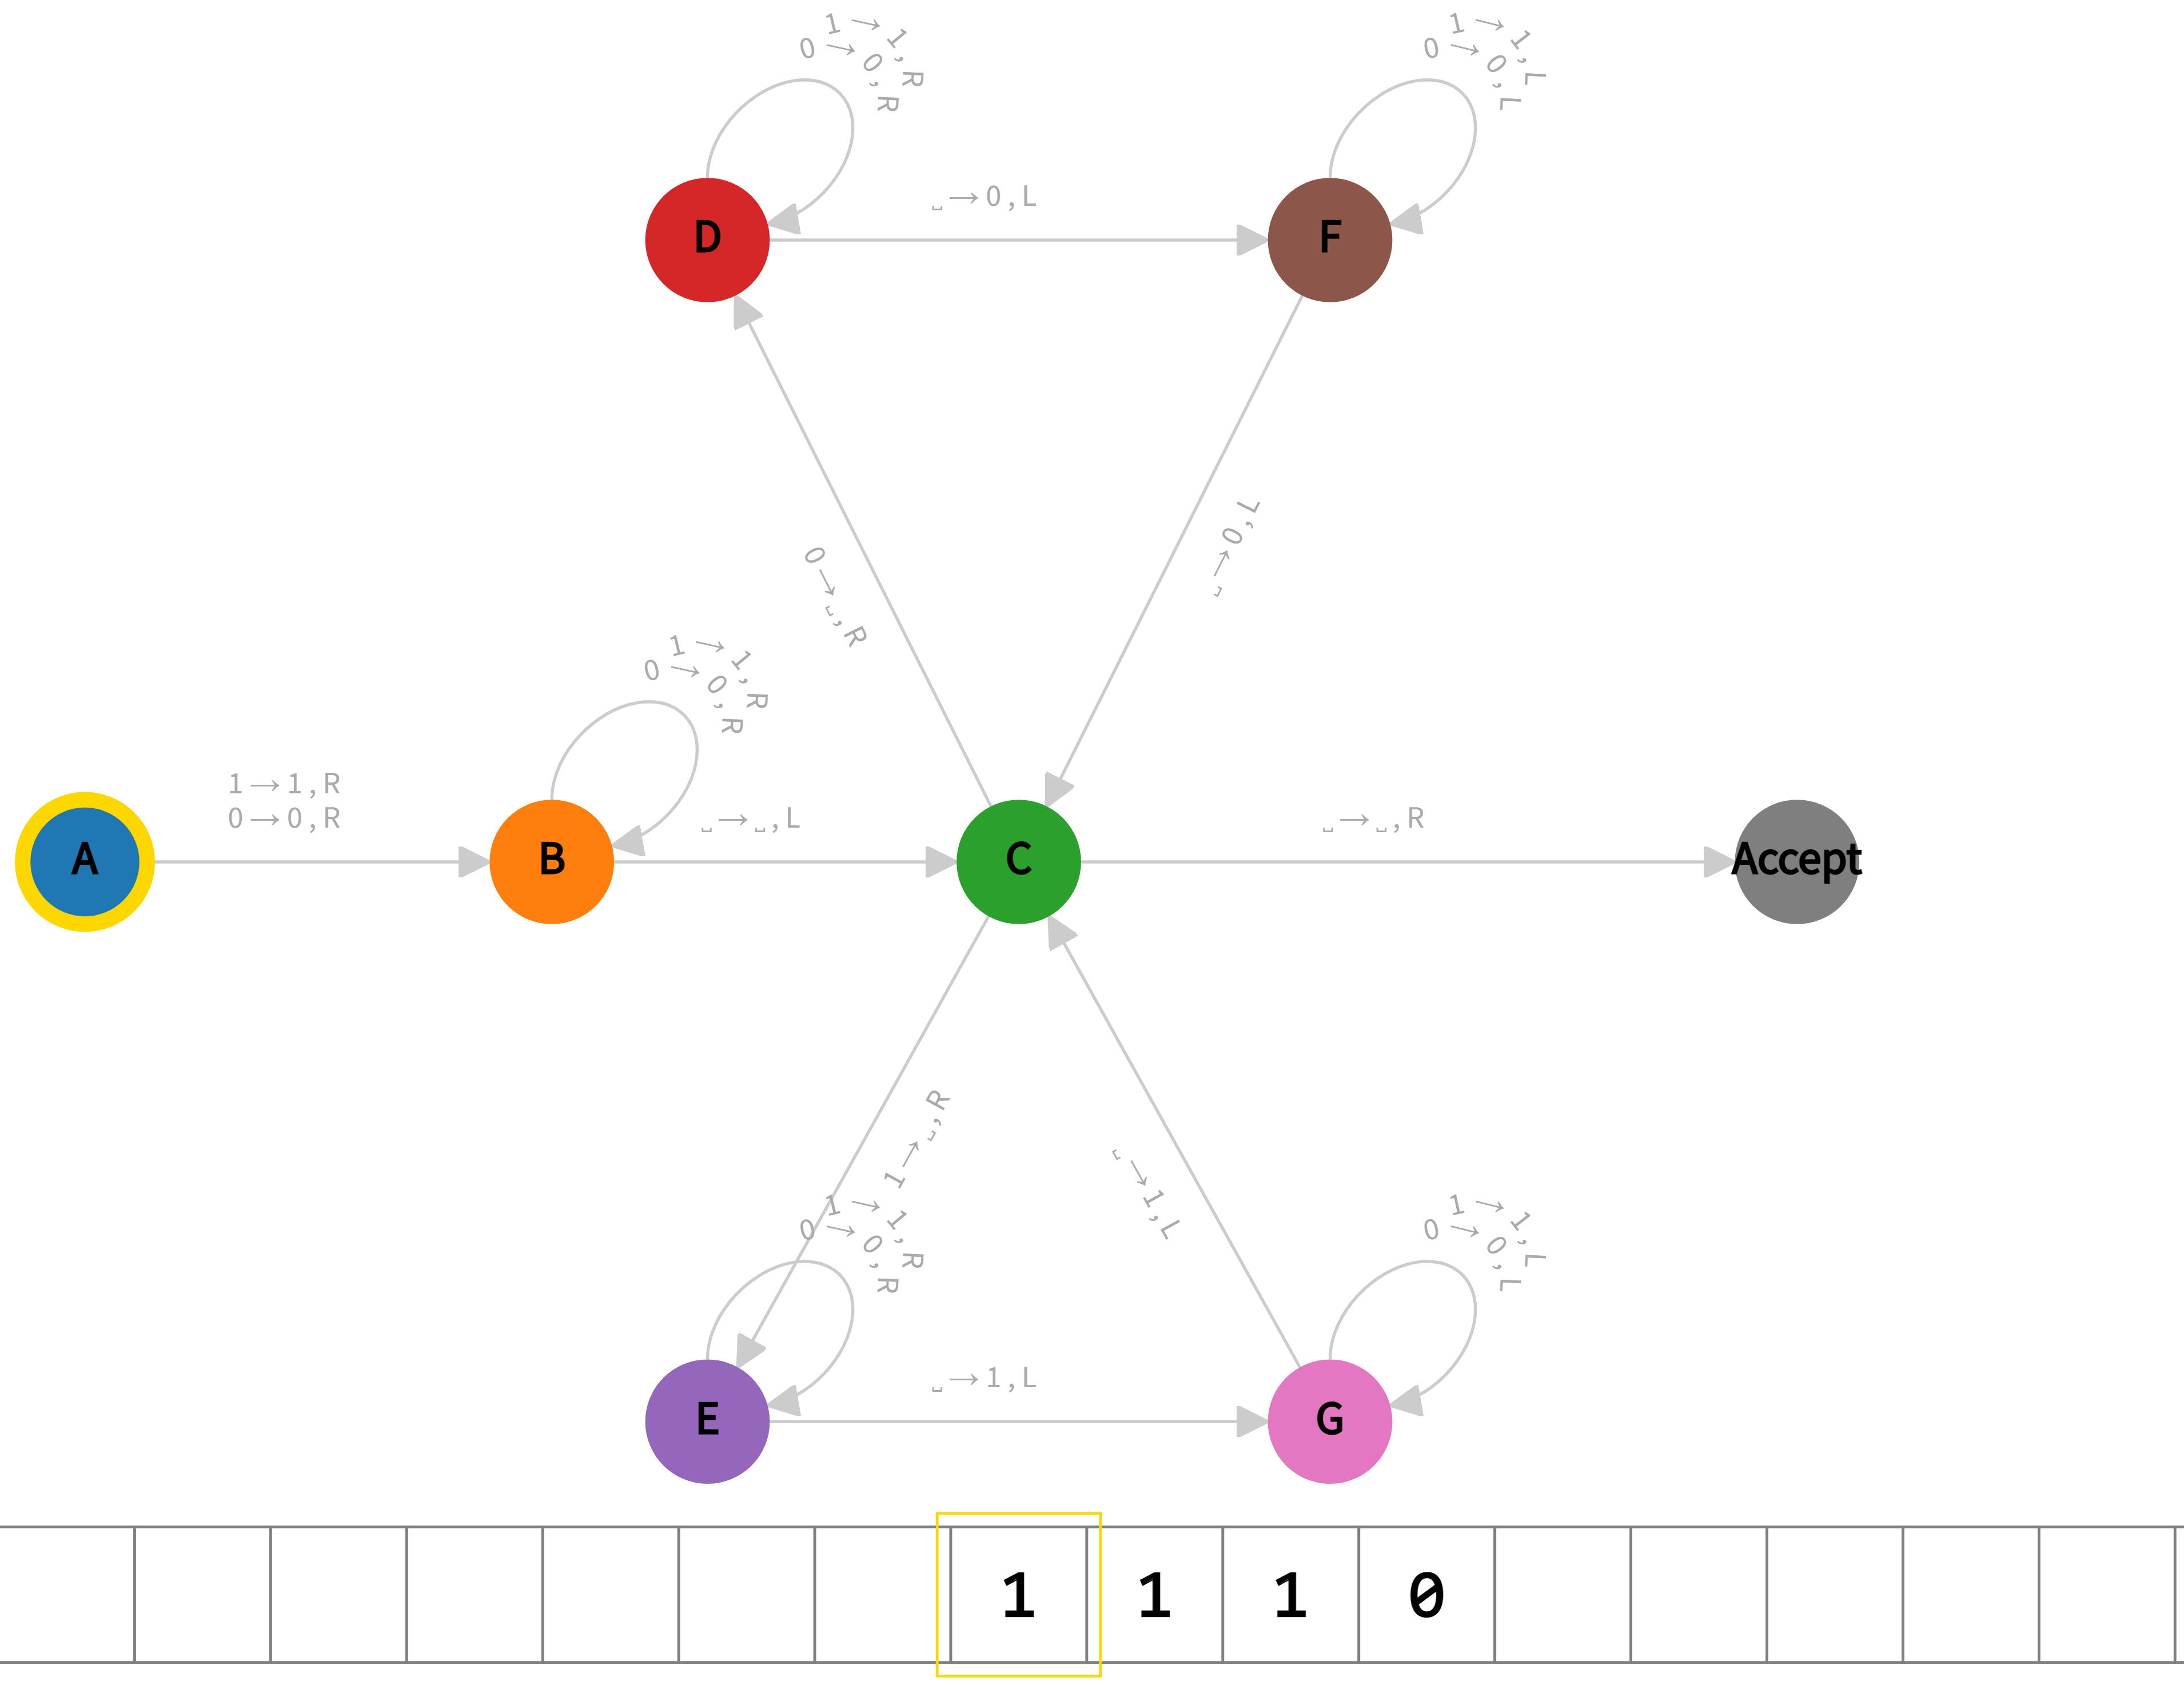
\includegraphics[width=\linewidth]{answers/img/q2-1110-initial.png}
    \caption*{Figure (a): Initial State for $\mathbf{1110}$}
    \label{fig:1110-initial}
  \end{minipage}
  \begin{minipage}{.49\linewidth}
    \centering
    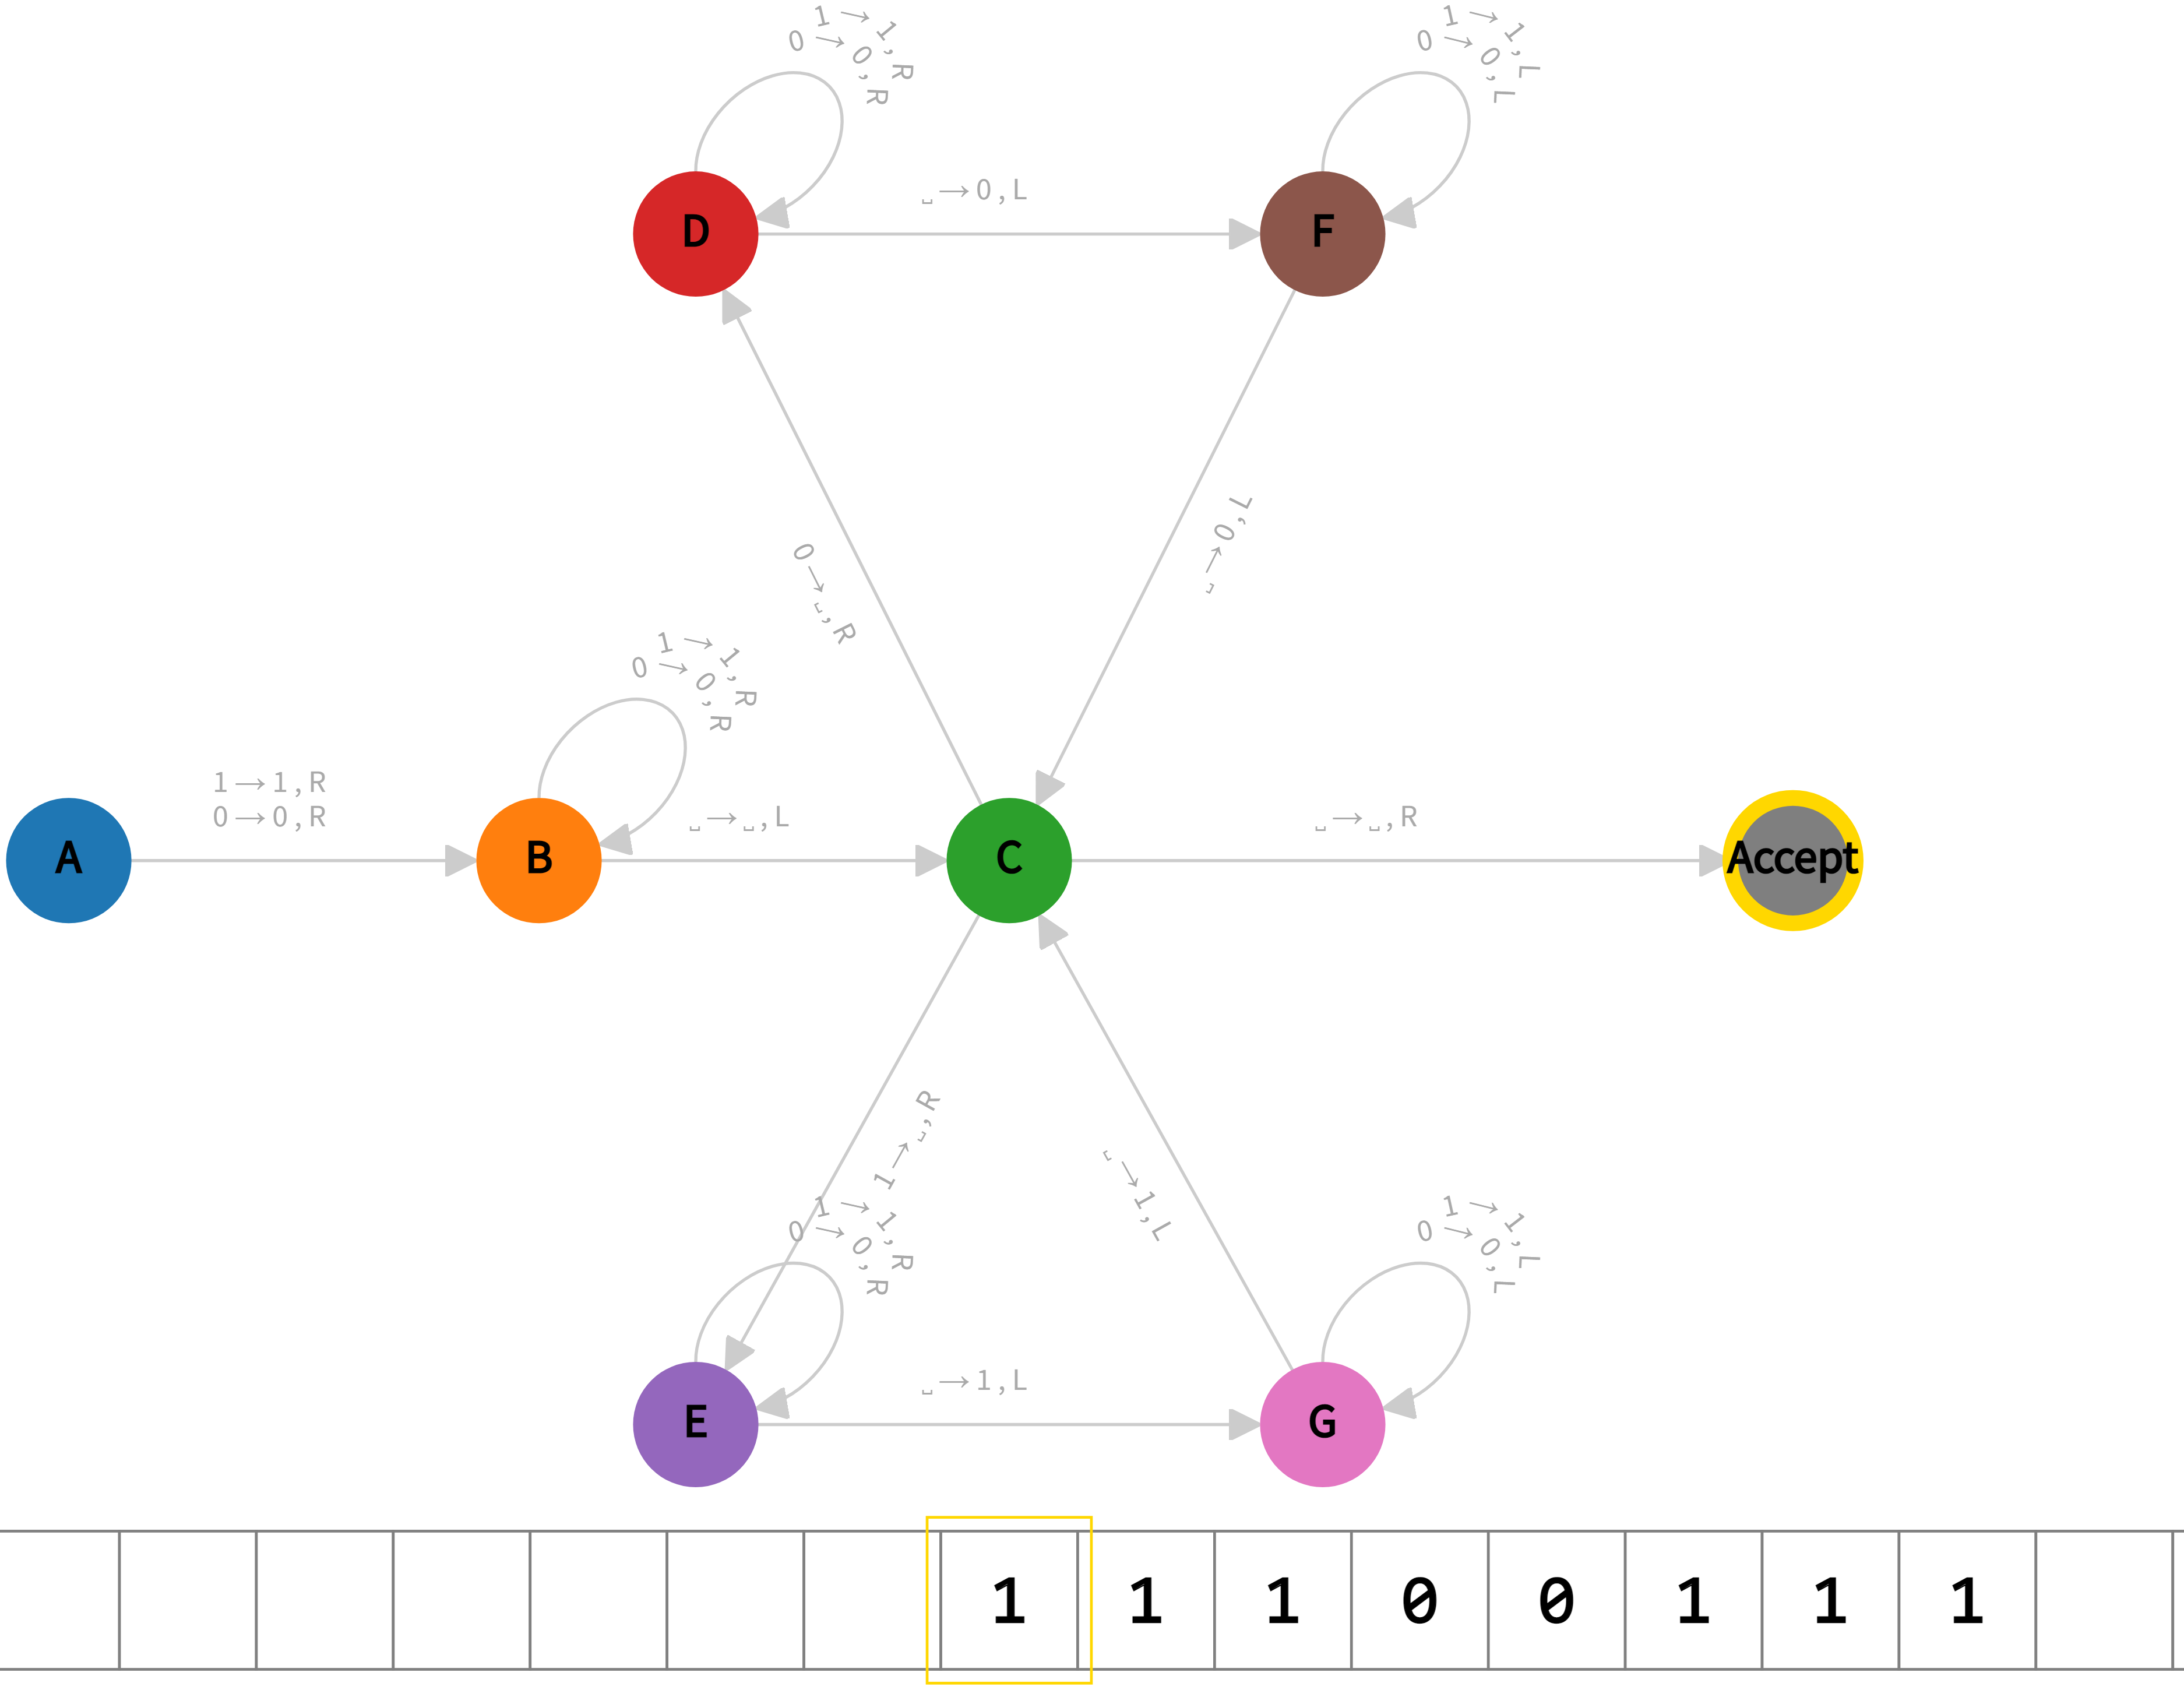
\includegraphics[width=\linewidth]{answers/img/q2-1110-end.png}
    \caption*{Figure (b): End State for $\mathbf{1110}$}
    \label{fig:1110-end}
  \end{minipage}
  \caption{States for $\mathbf{1110}$}
  \label{fig:in-1110}
\end{figure}

\vspace*{\fill}

\newpage

\vspace*{\fill}

\subsubsection*{Input: 0101}
\label{q2-0101}

\begin{figure}[ht]
  \centering
  \begin{minipage}{.49\linewidth}
    \centering
    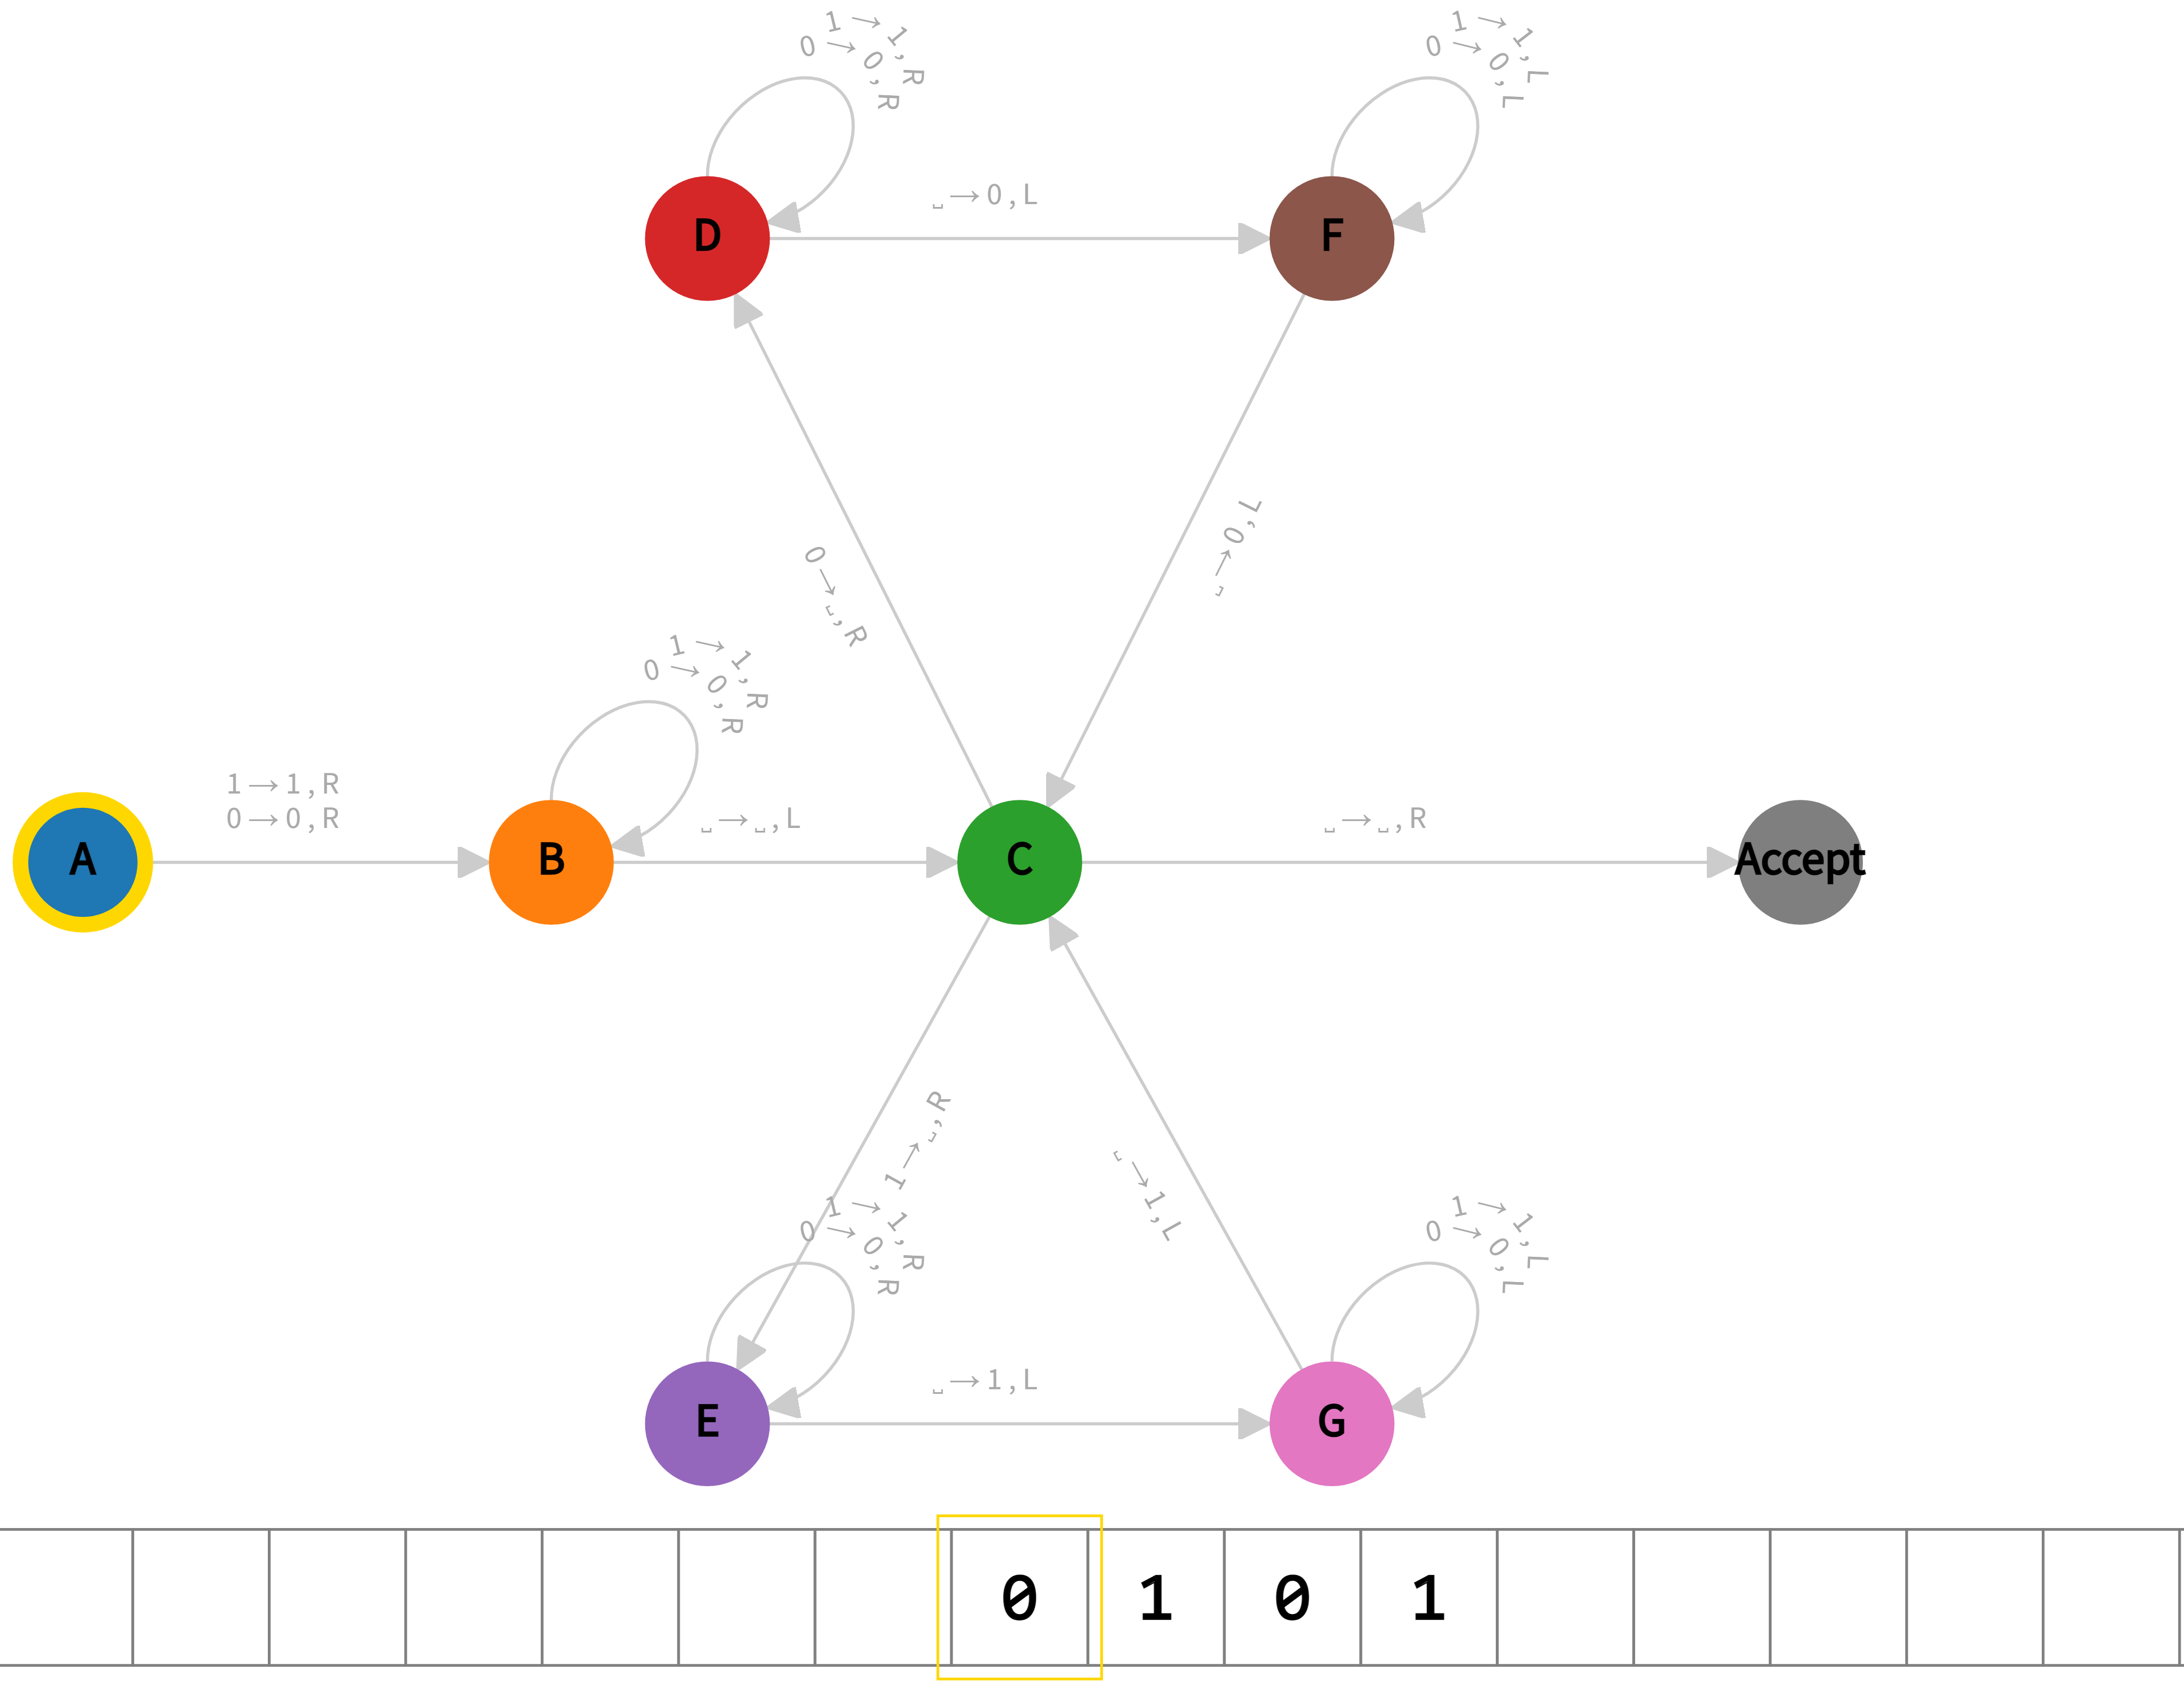
\includegraphics[width=\linewidth]{answers/img/q2-0101-initial.png}
    \caption*{Figure (a): Initial State for $\mathbf{0101}$}
    \label{fig:0101-initial}
  \end{minipage}
  \begin{minipage}{.49\linewidth}
    \centering
    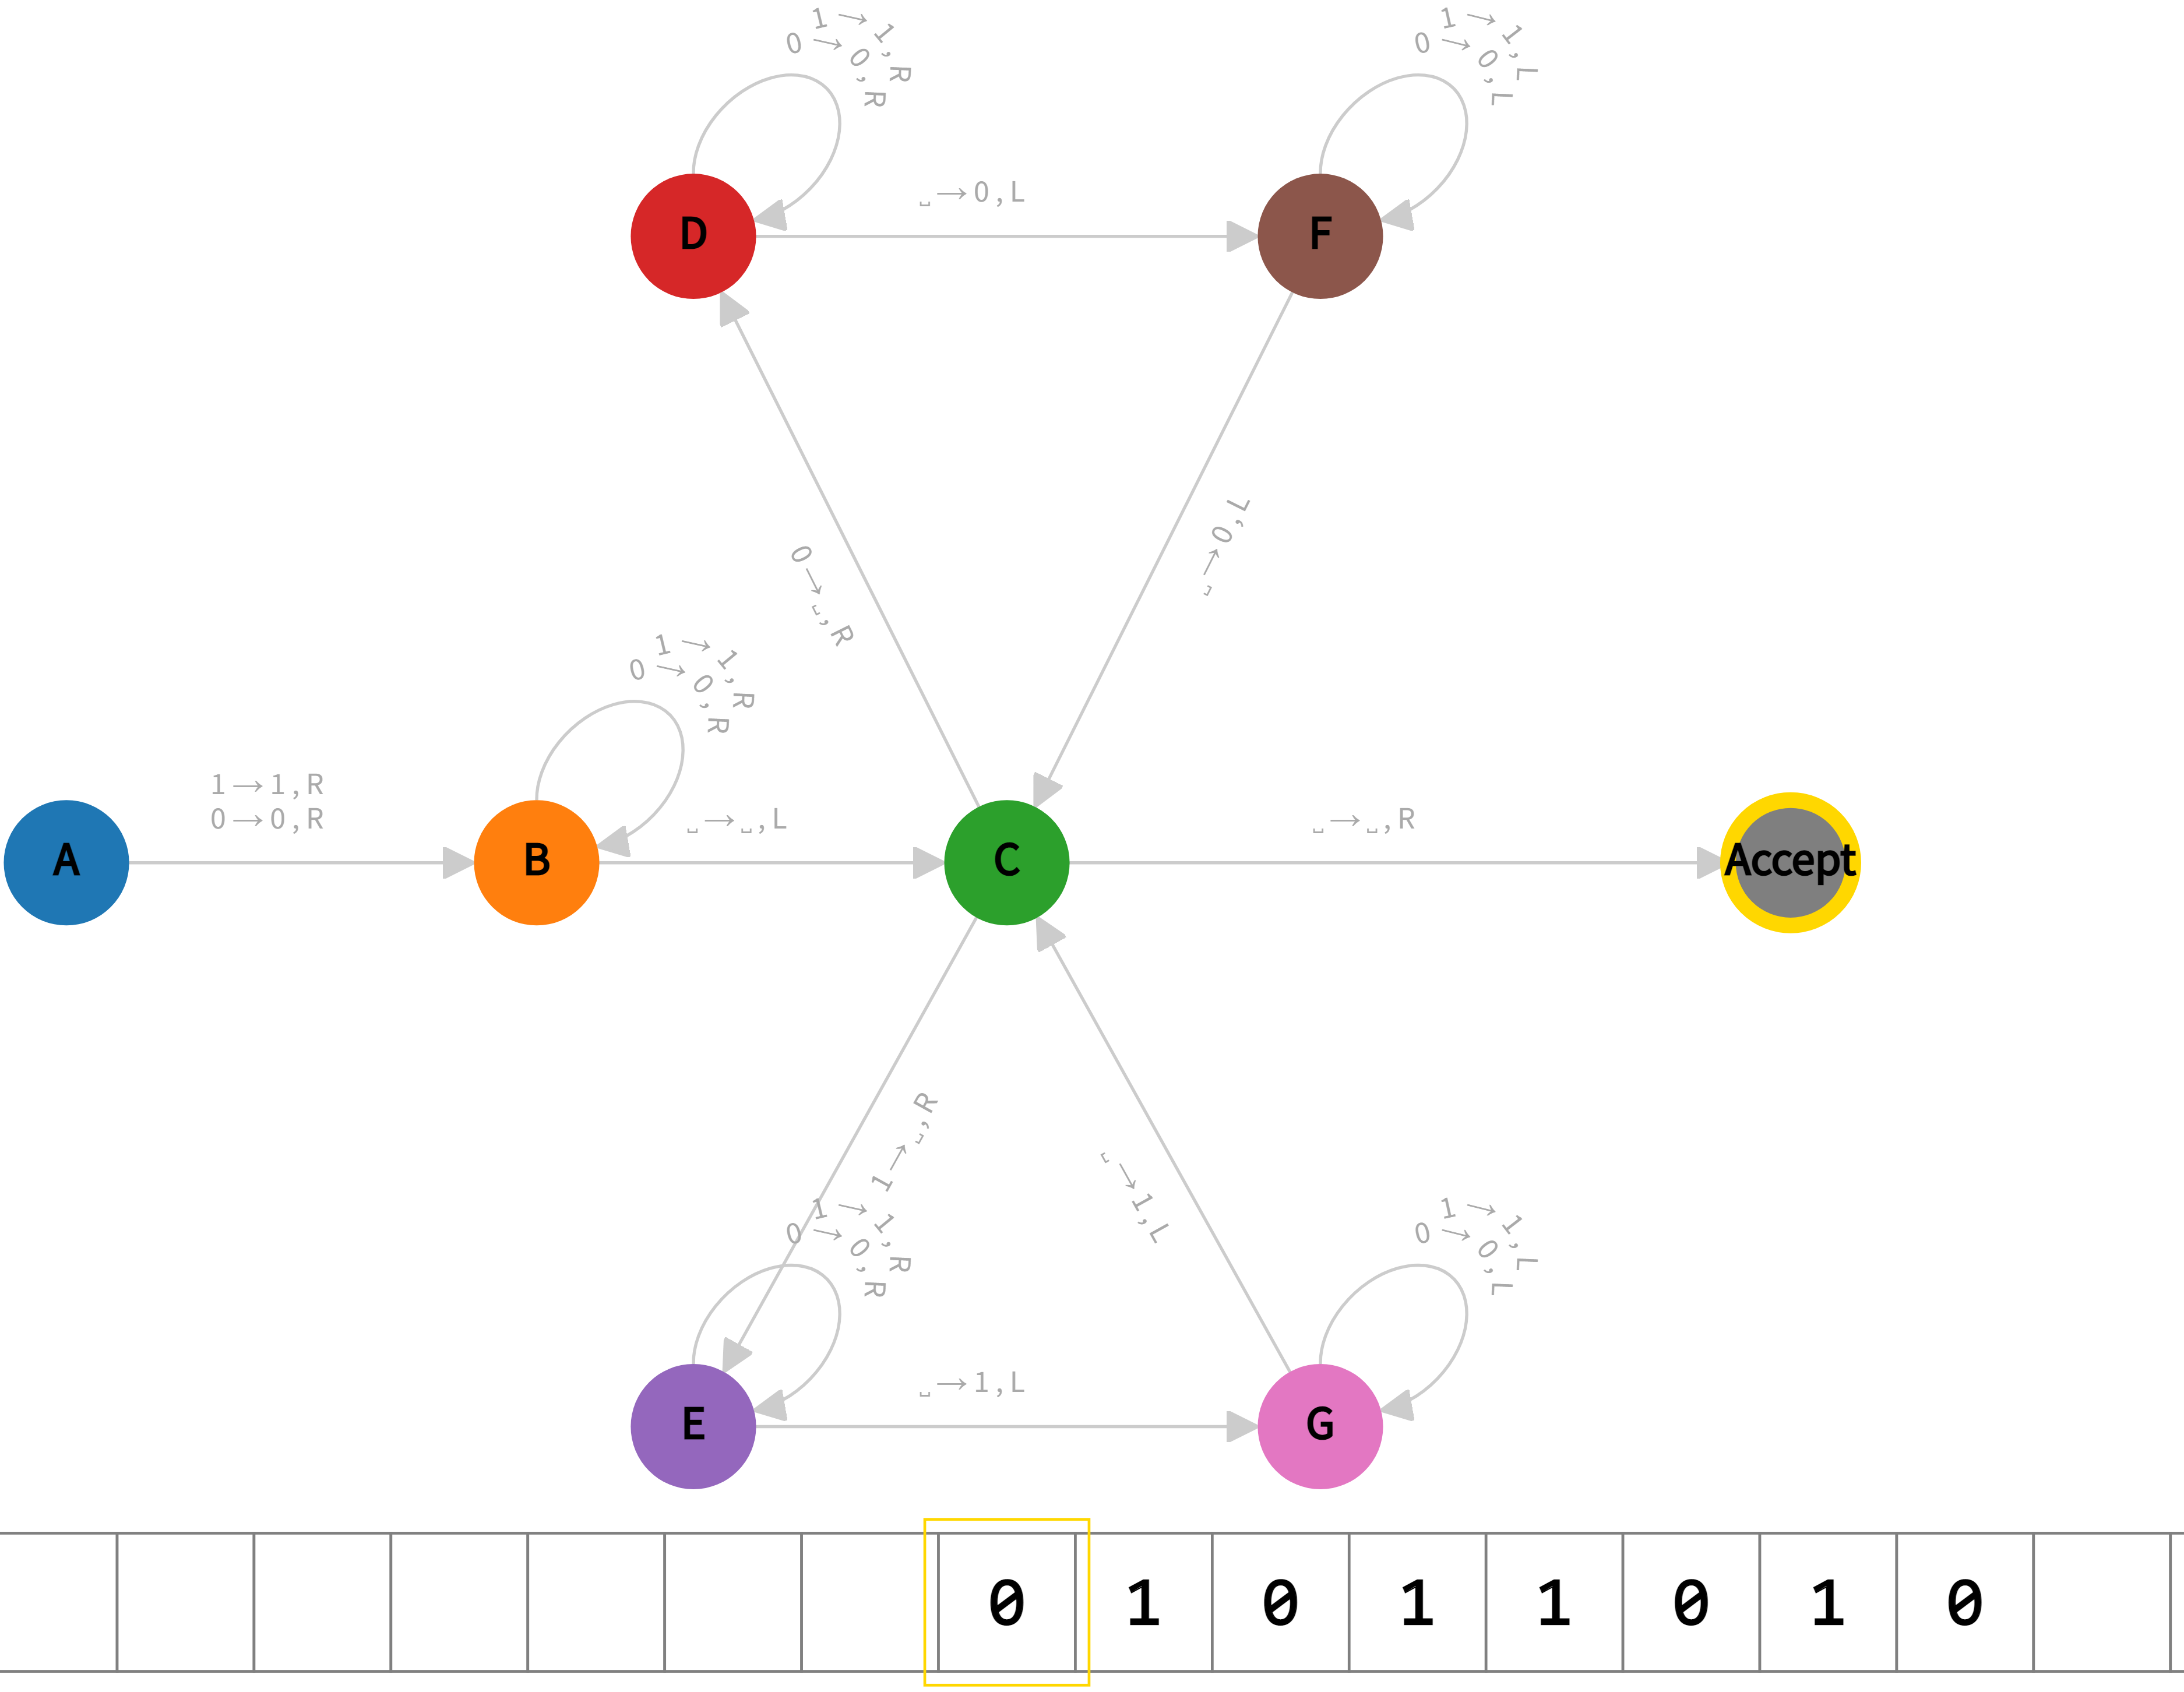
\includegraphics[width=\linewidth]{answers/img/q2-0101-end.png}
    \caption*{Figure (b): End State for $\mathbf{0101}$}
    \label{fig:0101-end}
  \end{minipage}
  \caption{States for $\mathbf{0101}$}
  \label{fig:in-0101}
\end{figure}

\subsubsection*{Input: 1010}
\label{q2-1010}

\begin{figure}[ht]
  \centering
  \begin{minipage}{.49\linewidth}
    \centering
    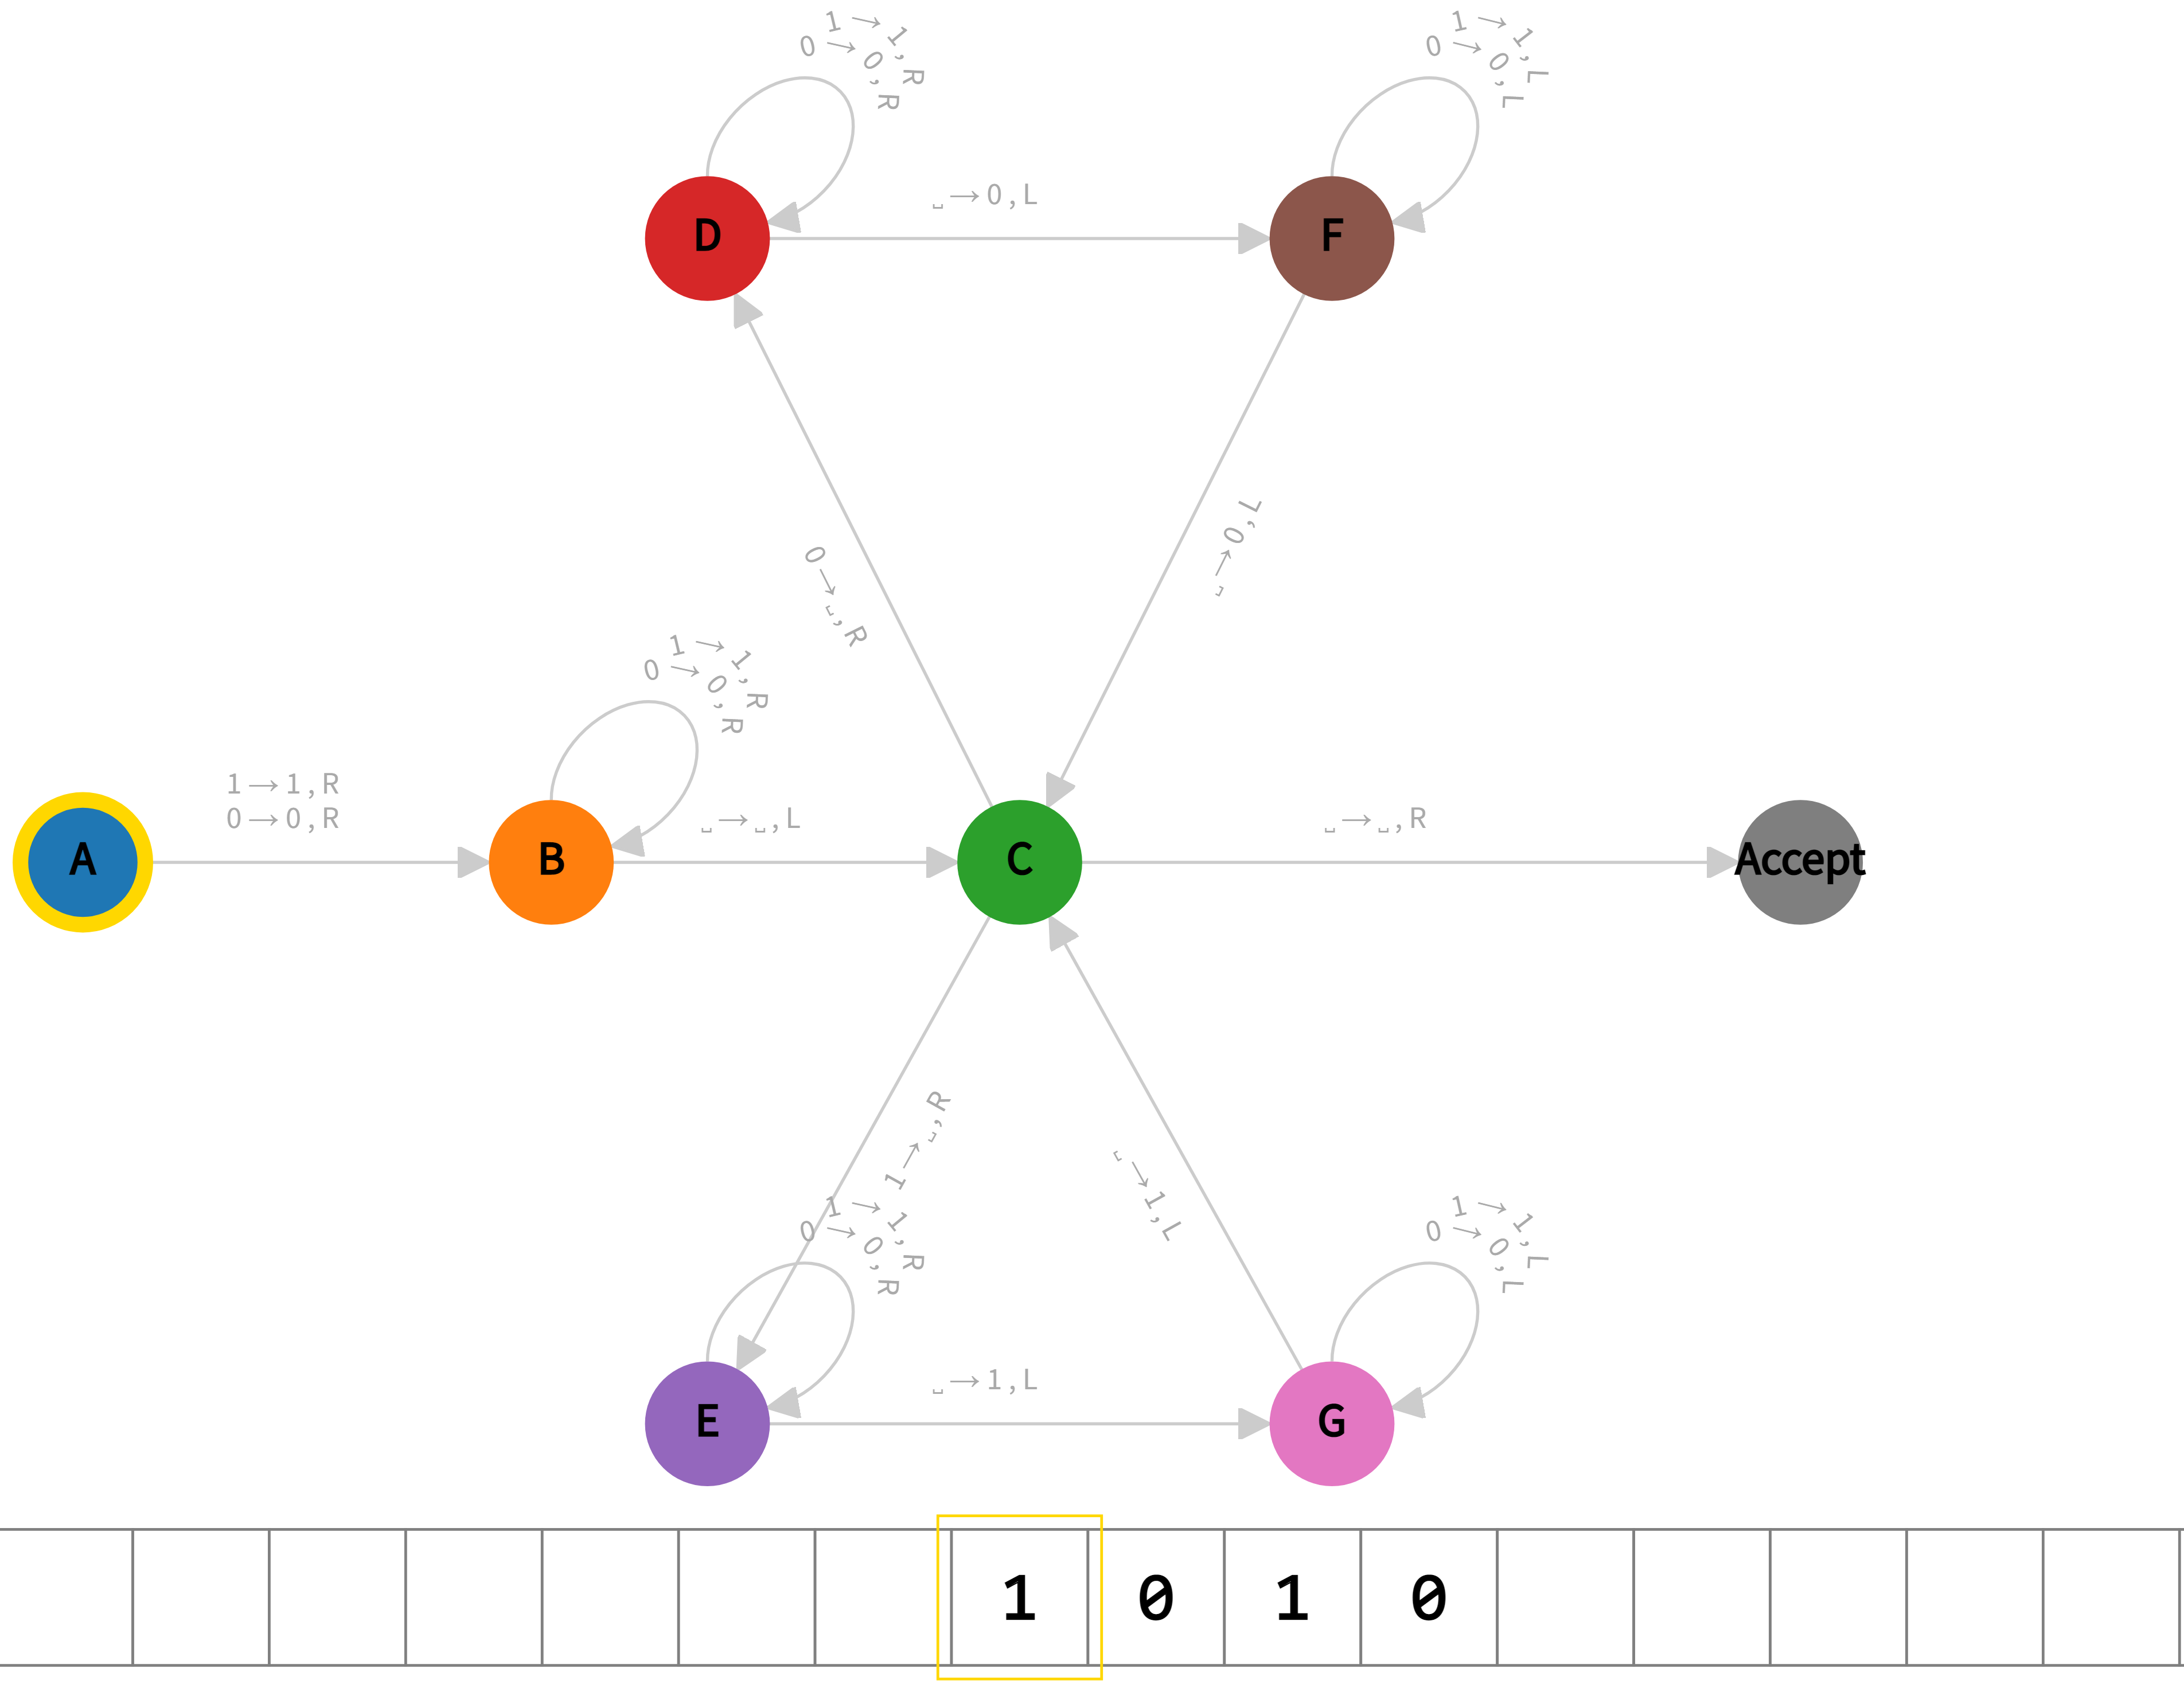
\includegraphics[width=\linewidth]{answers/img/q2-1010-initial.png}
    \caption*{Figure (a): Initial State for $\mathbf{1010}$}
    \label{fig:1010-initial}
  \end{minipage}
  \begin{minipage}{.49\linewidth}
    \centering
    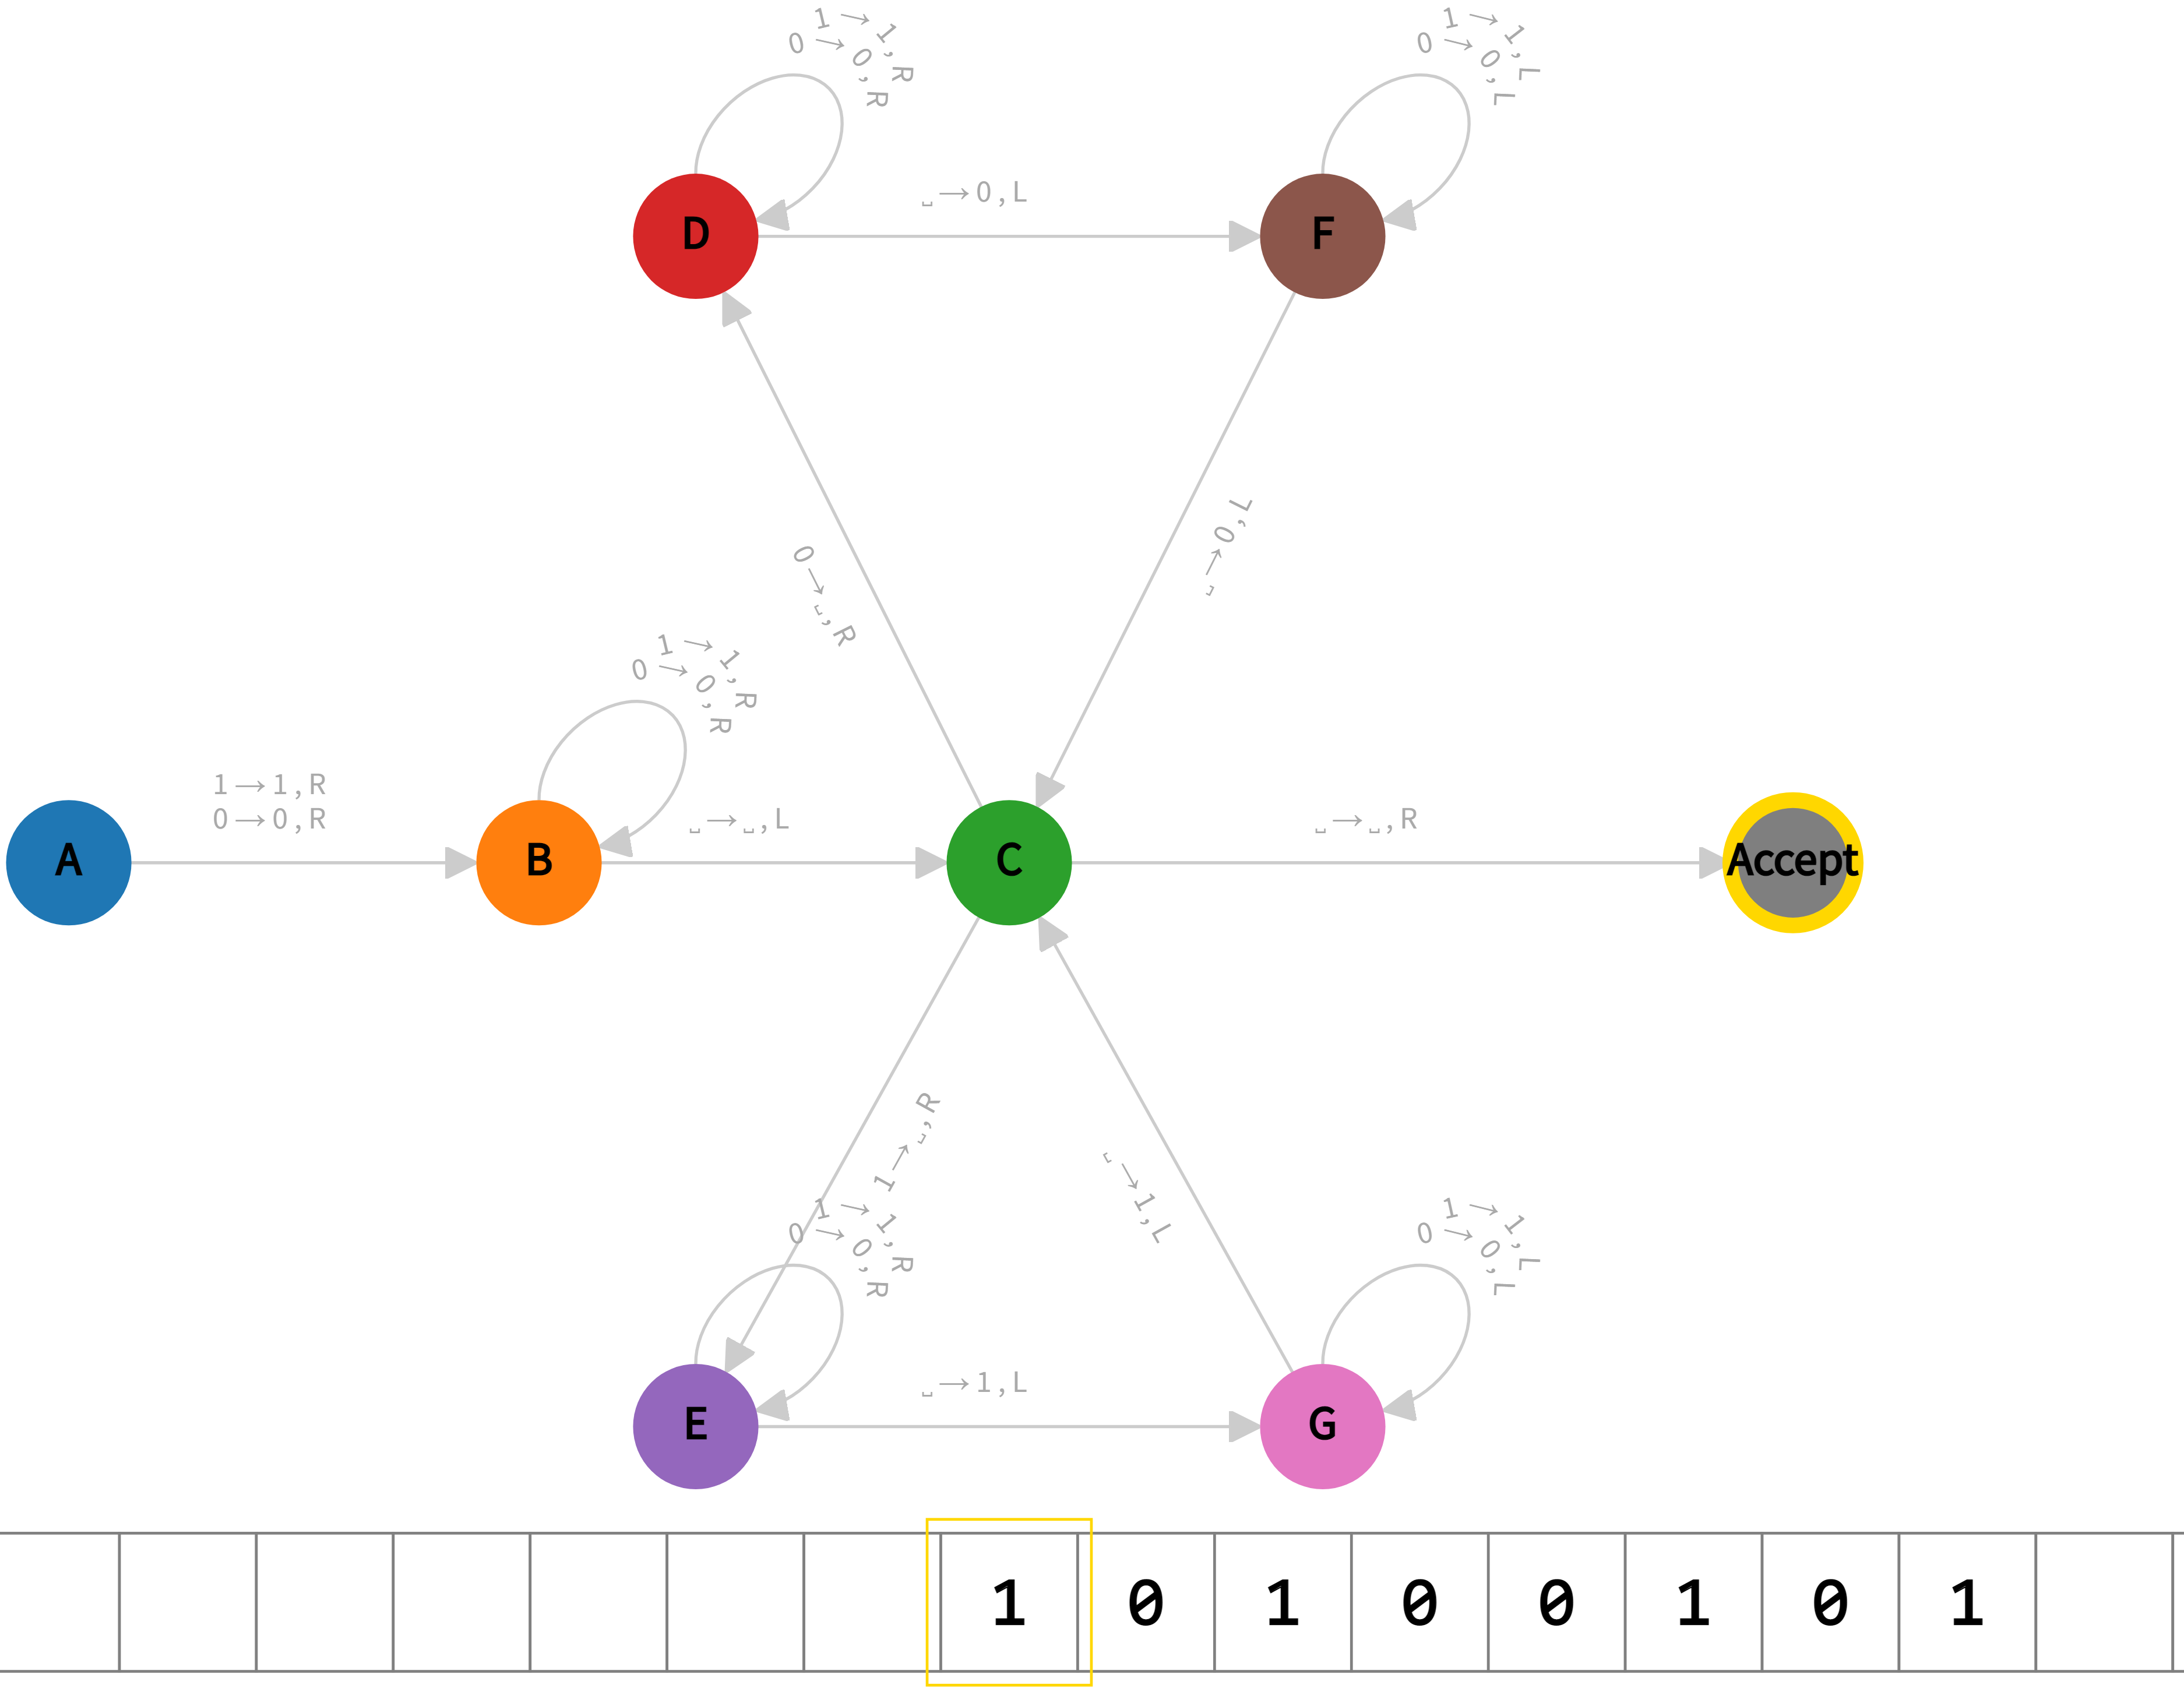
\includegraphics[width=\linewidth]{answers/img/q2-1010-end.png}
    \caption*{Figure (b): End State for $\mathbf{1010}$}
    \label{fig:1010-end}
  \end{minipage}
  \caption{States for $\mathbf{1010}$}
  \label{fig:in-1010}
\end{figure}

\vspace*{\fill}
\newpage
\vspace*{\fill}

\subsection*{Input: 1010001}

\begin{figure}[ht]
  \centering
  \begin{minipage}{.49\linewidth}
    \centering
    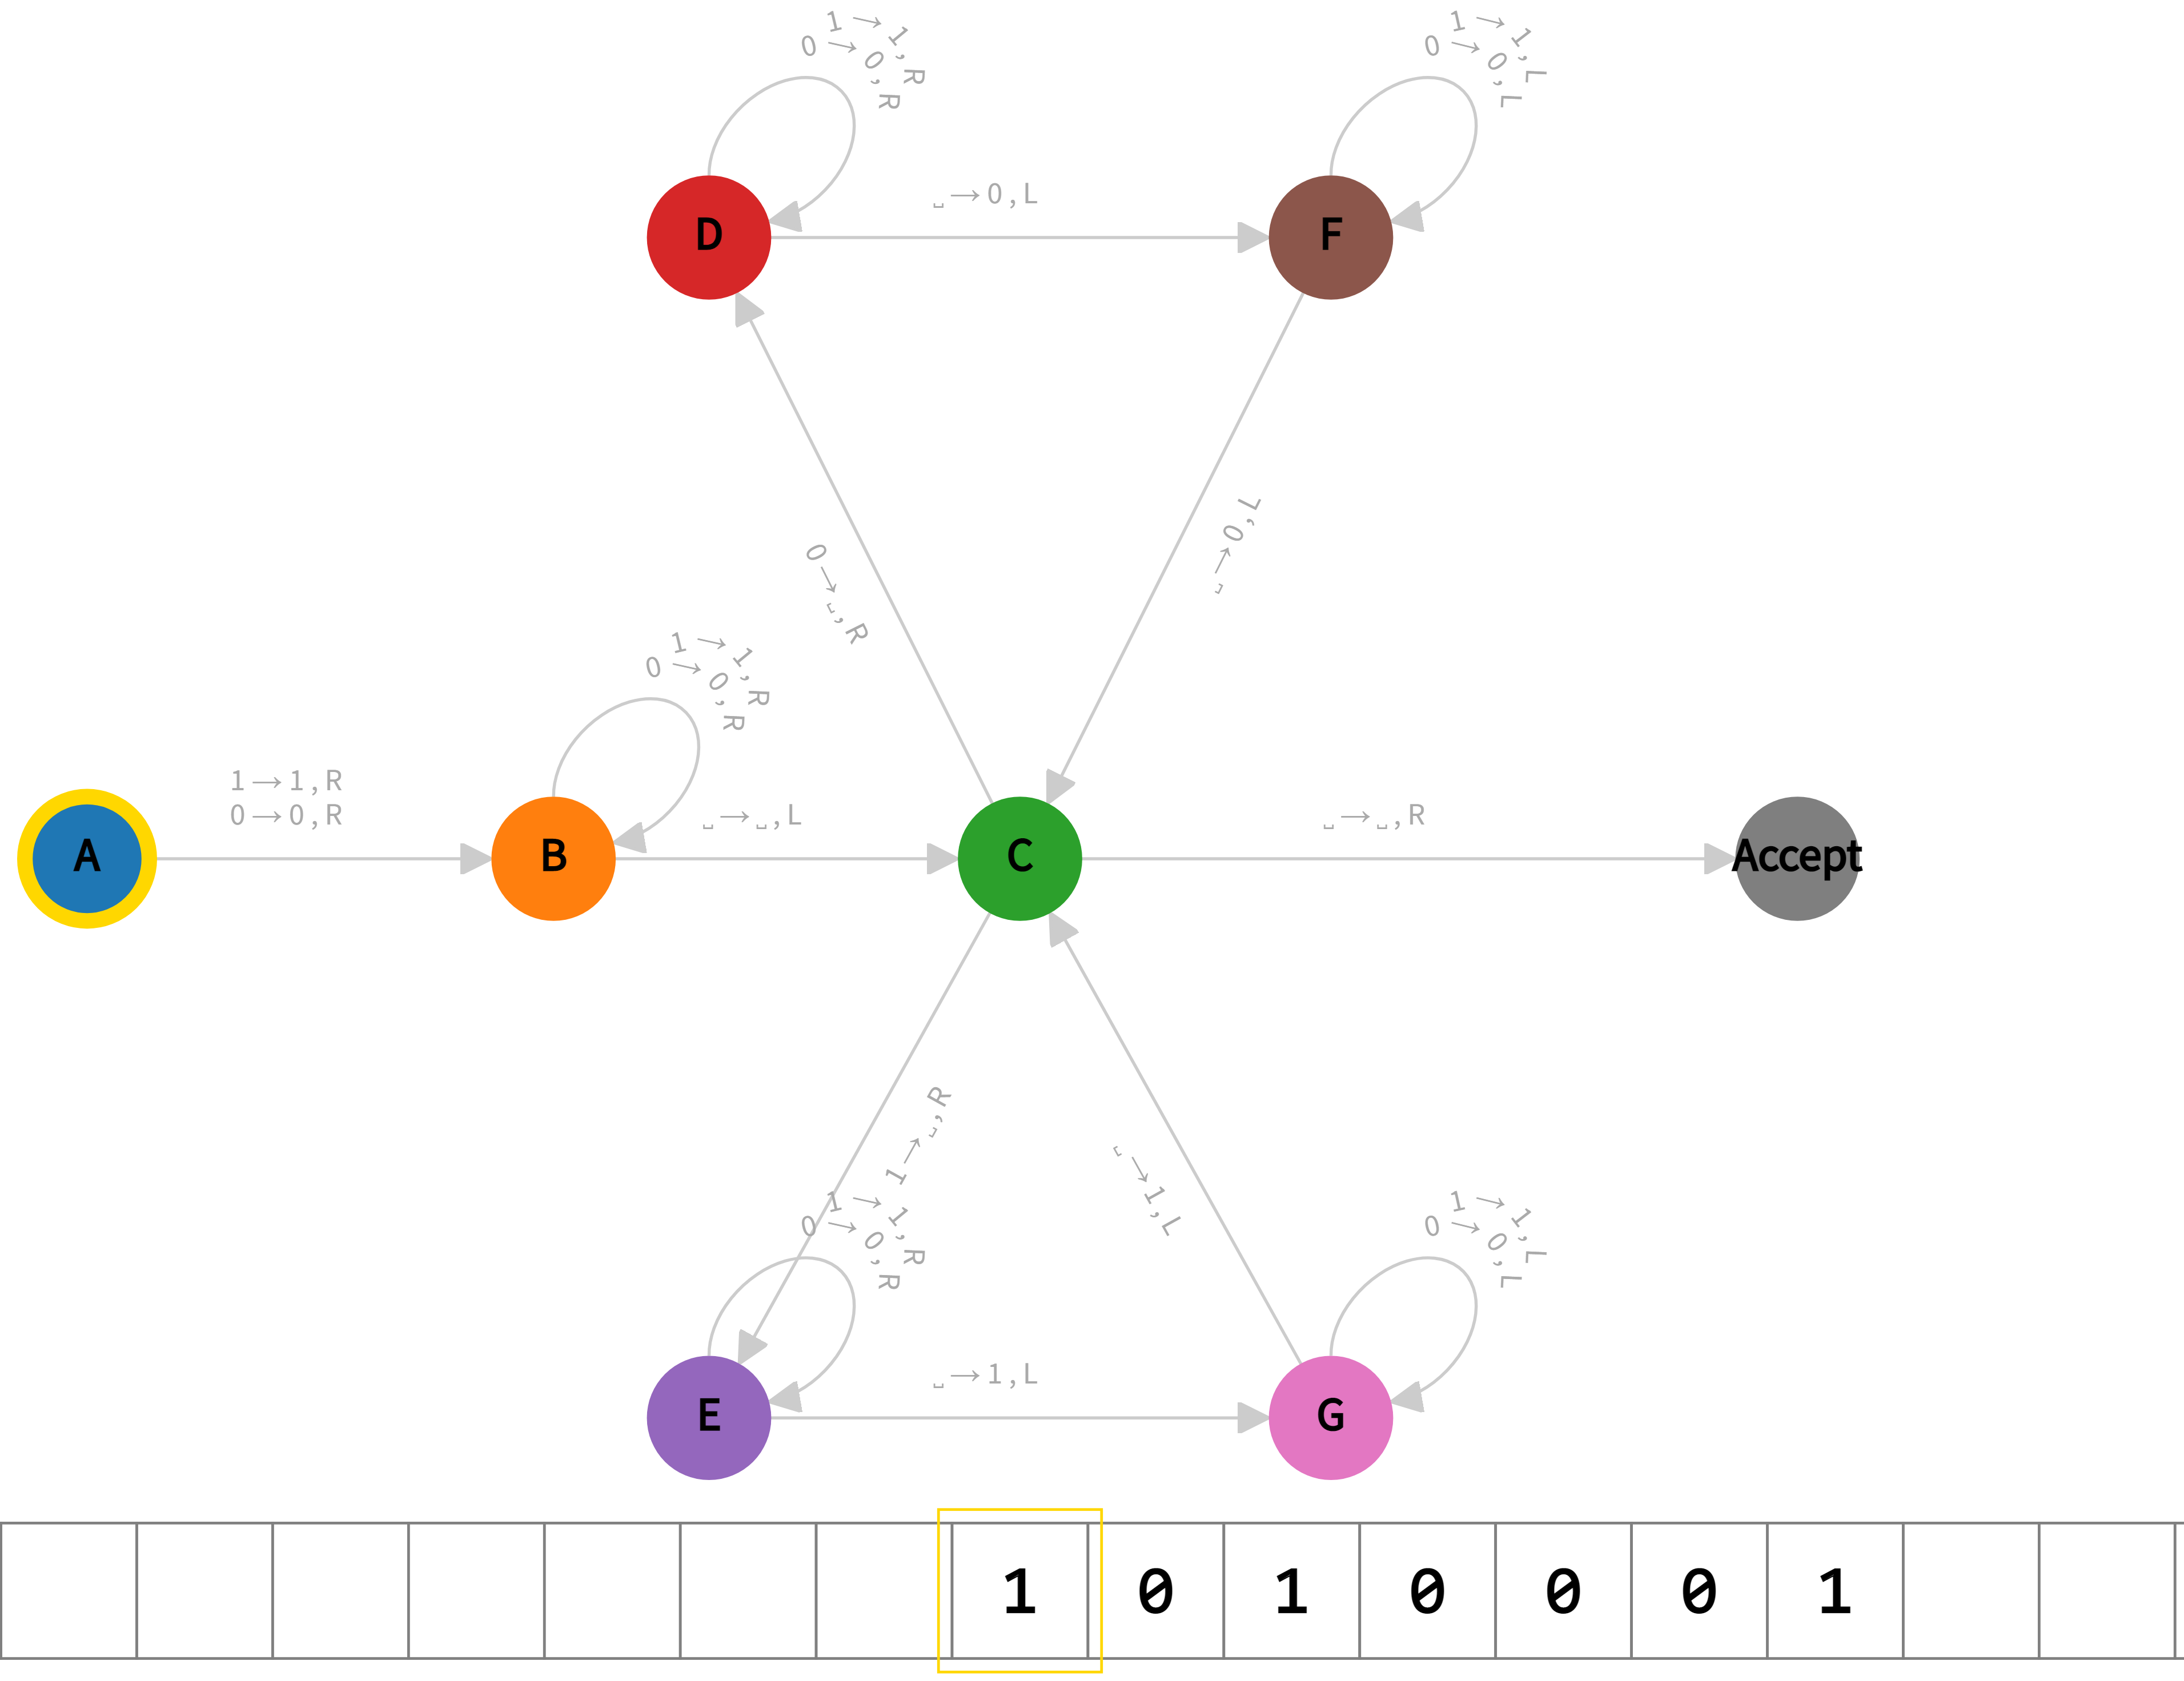
\includegraphics[width=\linewidth]{answers/img/q2-1010001-initial.png}
    \caption*{Figure (a): Initial State for $\mathbf{1010001}$}
    \label{fig:1010001-initial}
  \end{minipage}
  \begin{minipage}{.49\linewidth}
    \centering
    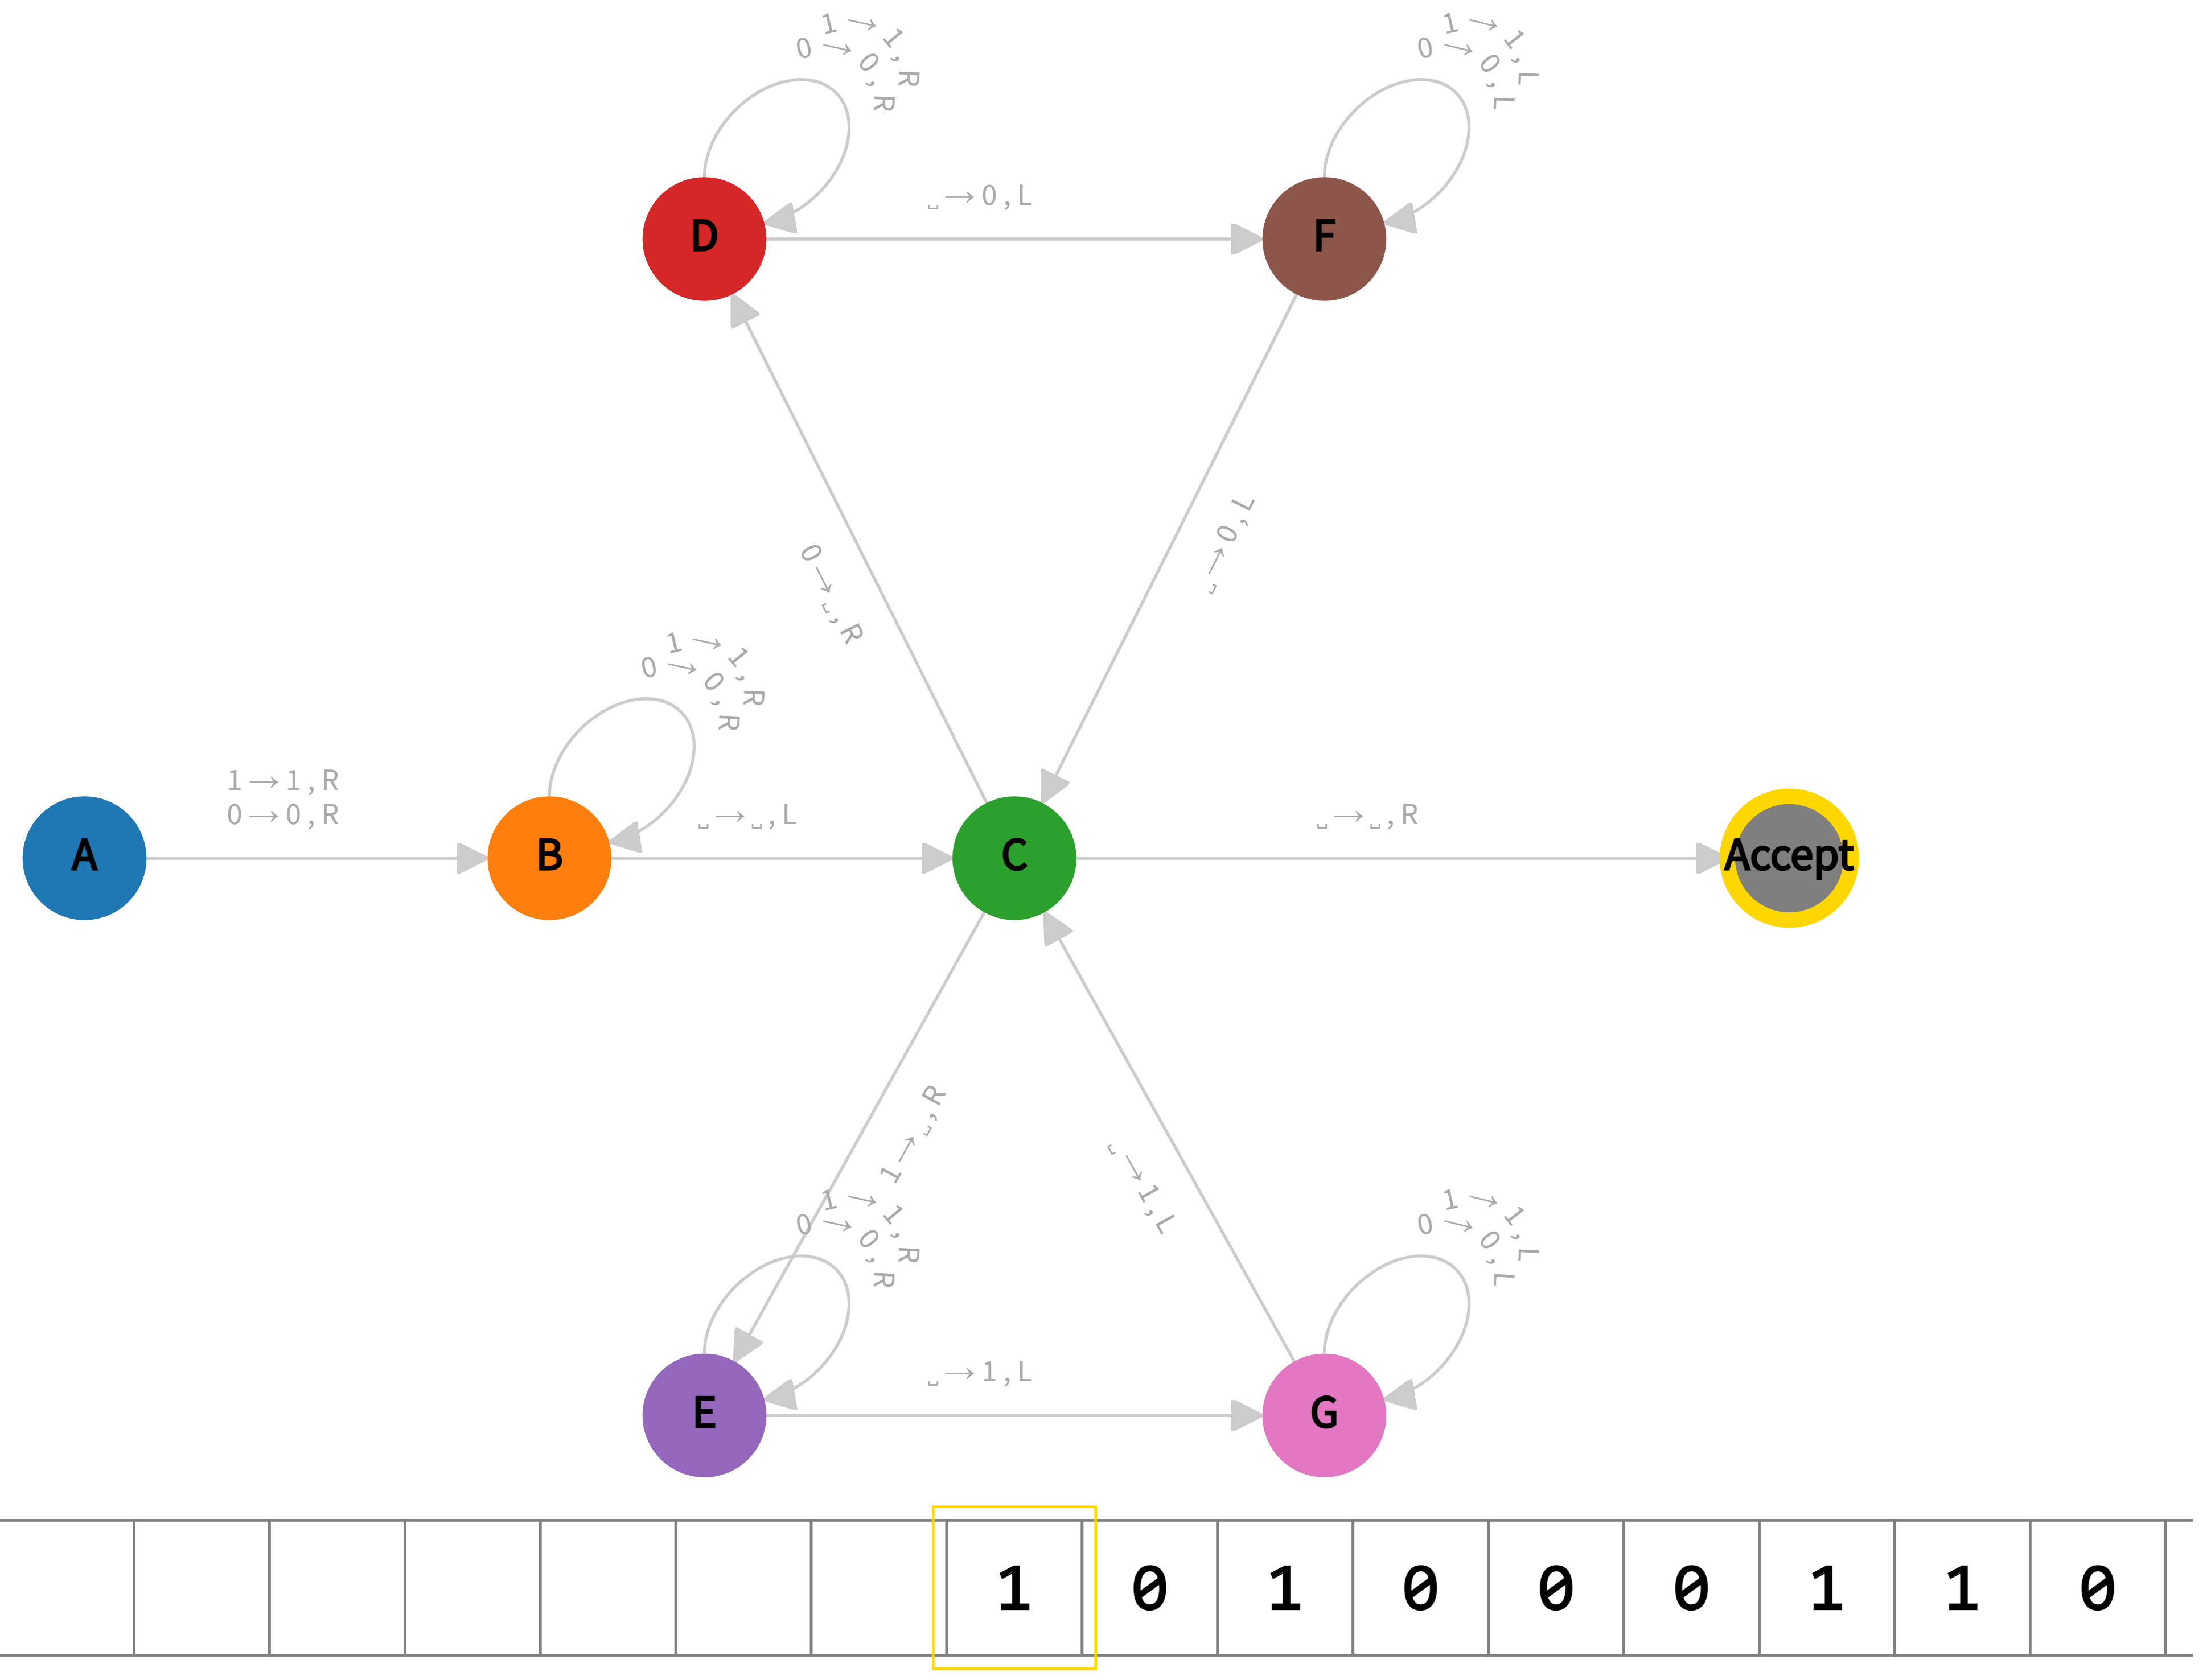
\includegraphics[width=\linewidth]{answers/img/q2-1010001-end.png}
    \caption*{Figure (b): End State for $\mathbf{1010001}$}
    \label{fig:1010001-end}
  \end{minipage}
  \caption{States for $\mathbf{1010001}$}
  \label{fig:in-1010001}
\end{figure}

\begin{center}
\textbf{\textit{Due to the head place, the whole output cannot be seen in \hyperref[fig:1010001-end]{Figure 13.b}.}}
\end{center}

\subsection*{Input: 00111}

\begin{figure}[ht]
  \centering
  \begin{minipage}{.49\linewidth}
    \centering
    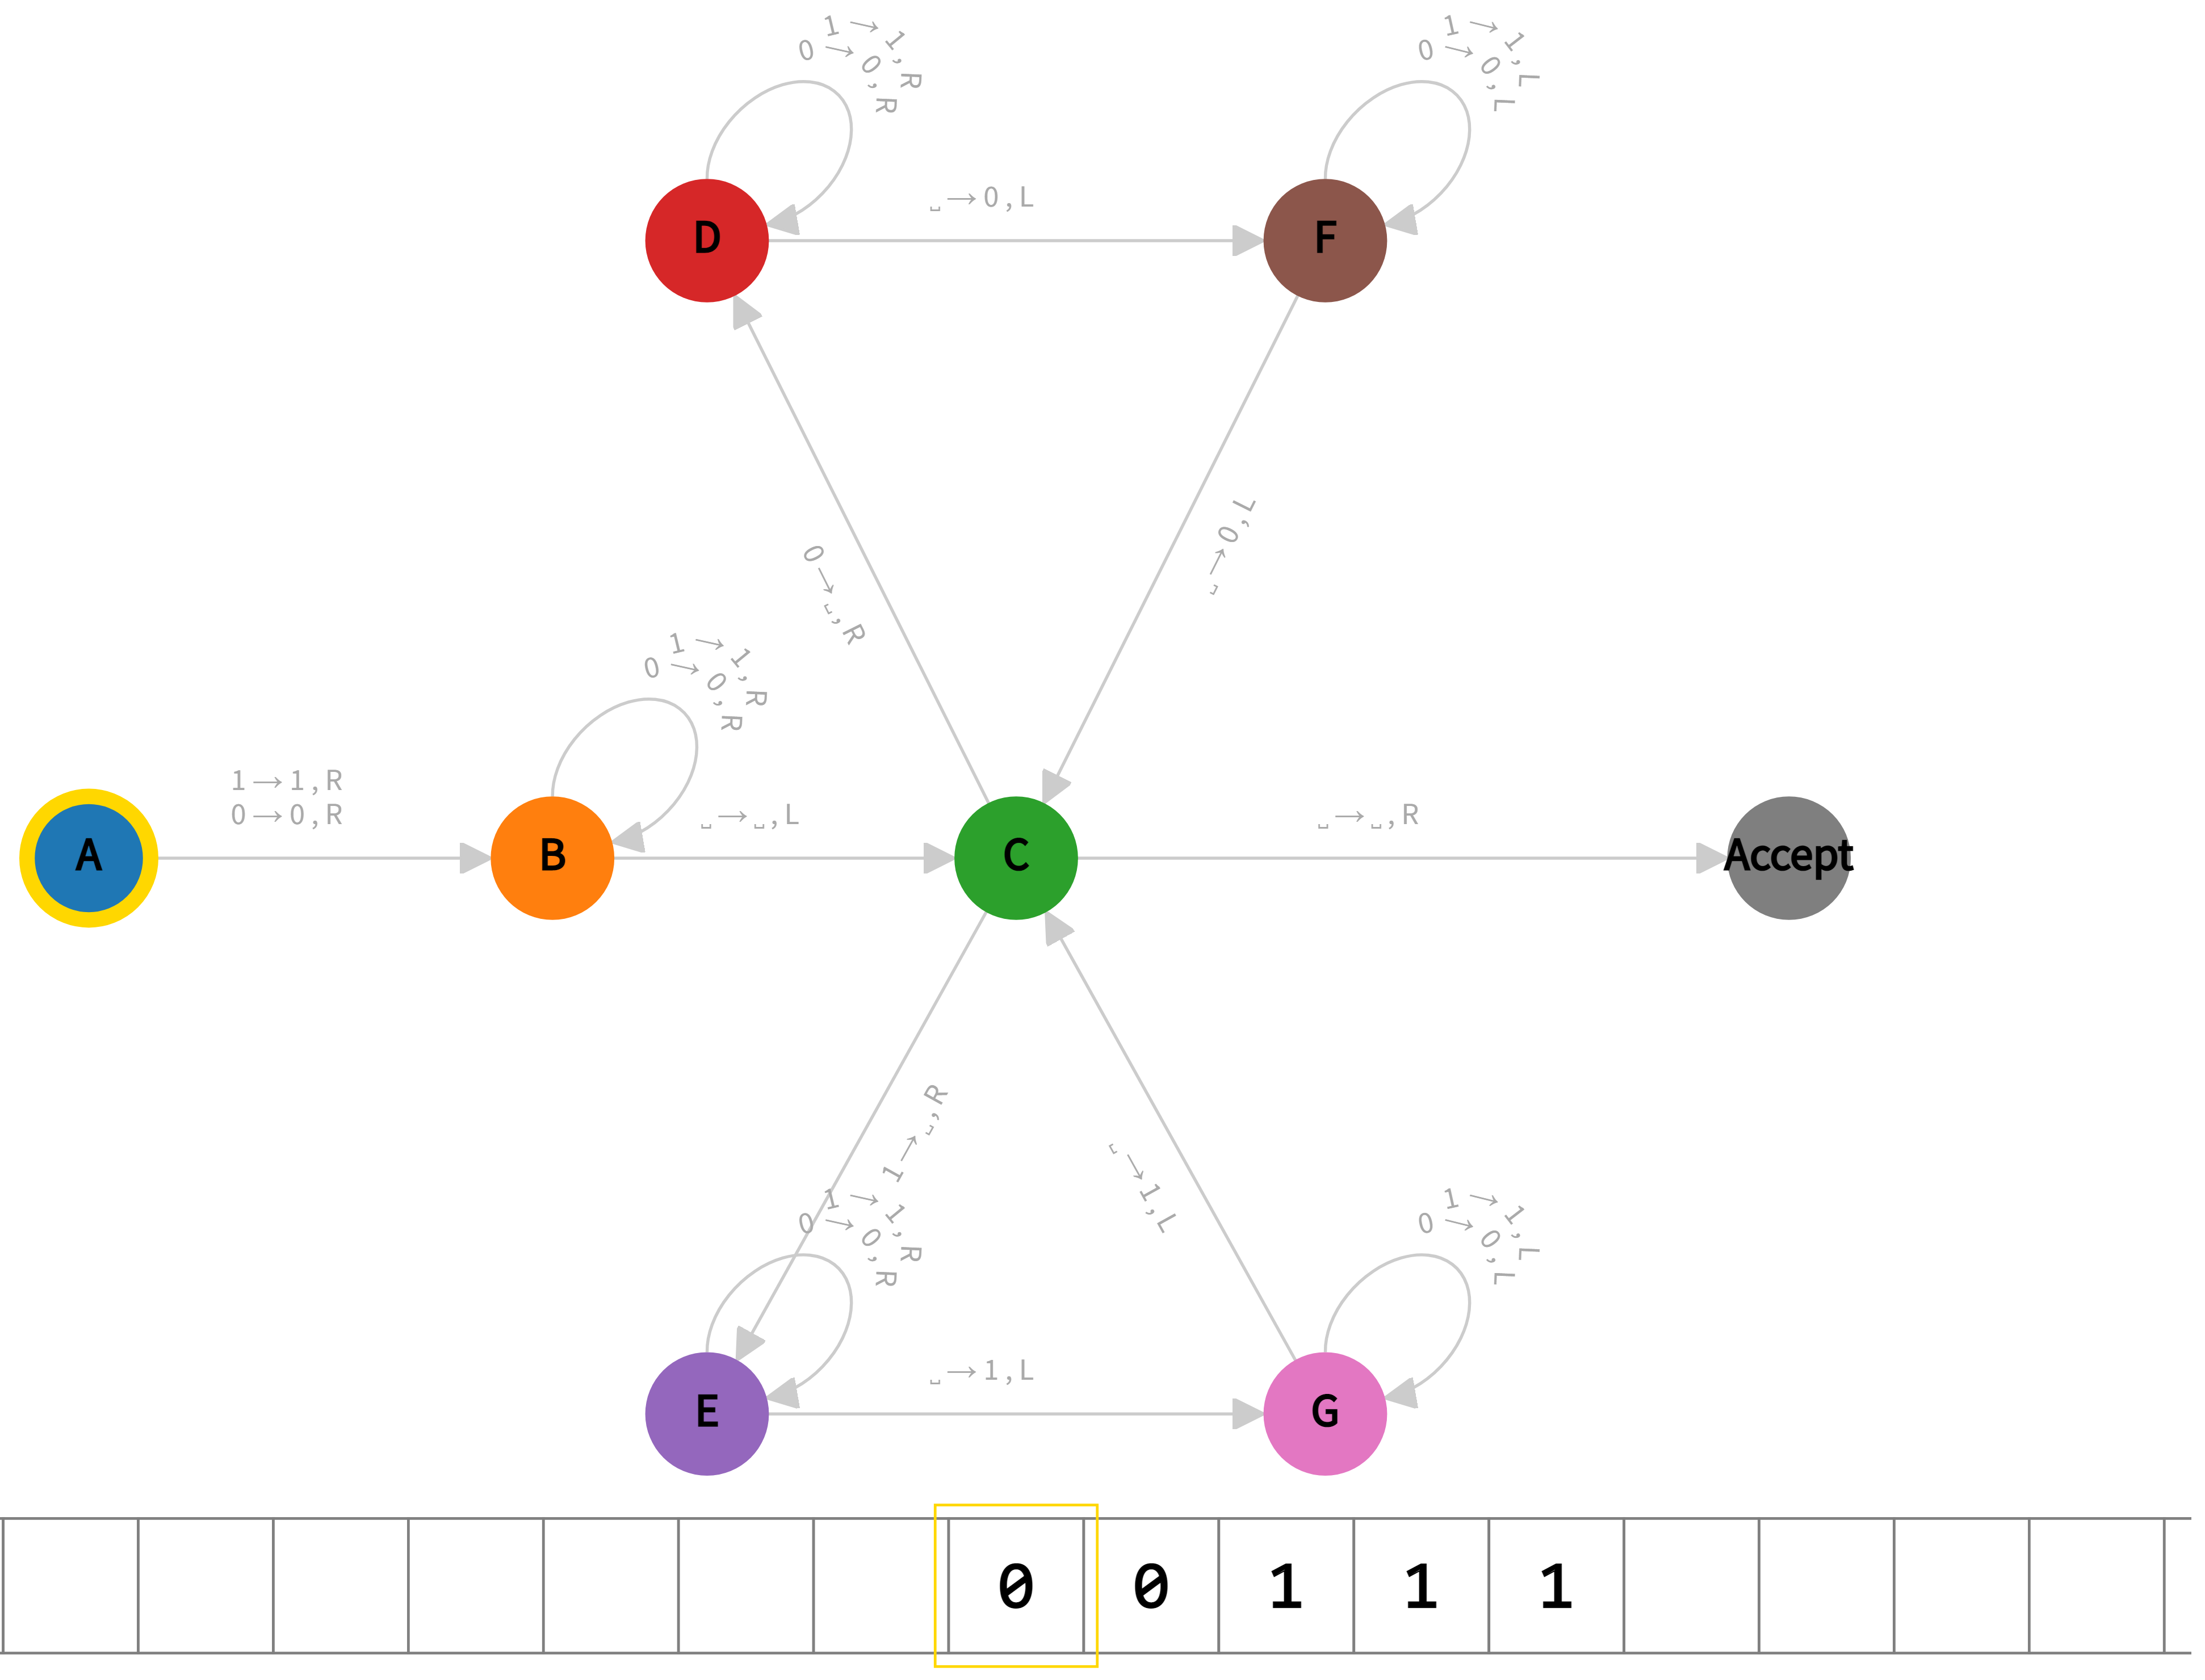
\includegraphics[width=\linewidth]{answers/img/q2-00111-initial.png}
    \caption*{Figure (a): Initial State for $\mathbf{00111}$}
    \label{fig:00111-initial}
  \end{minipage}
  \begin{minipage}{.49\linewidth}
    \centering
    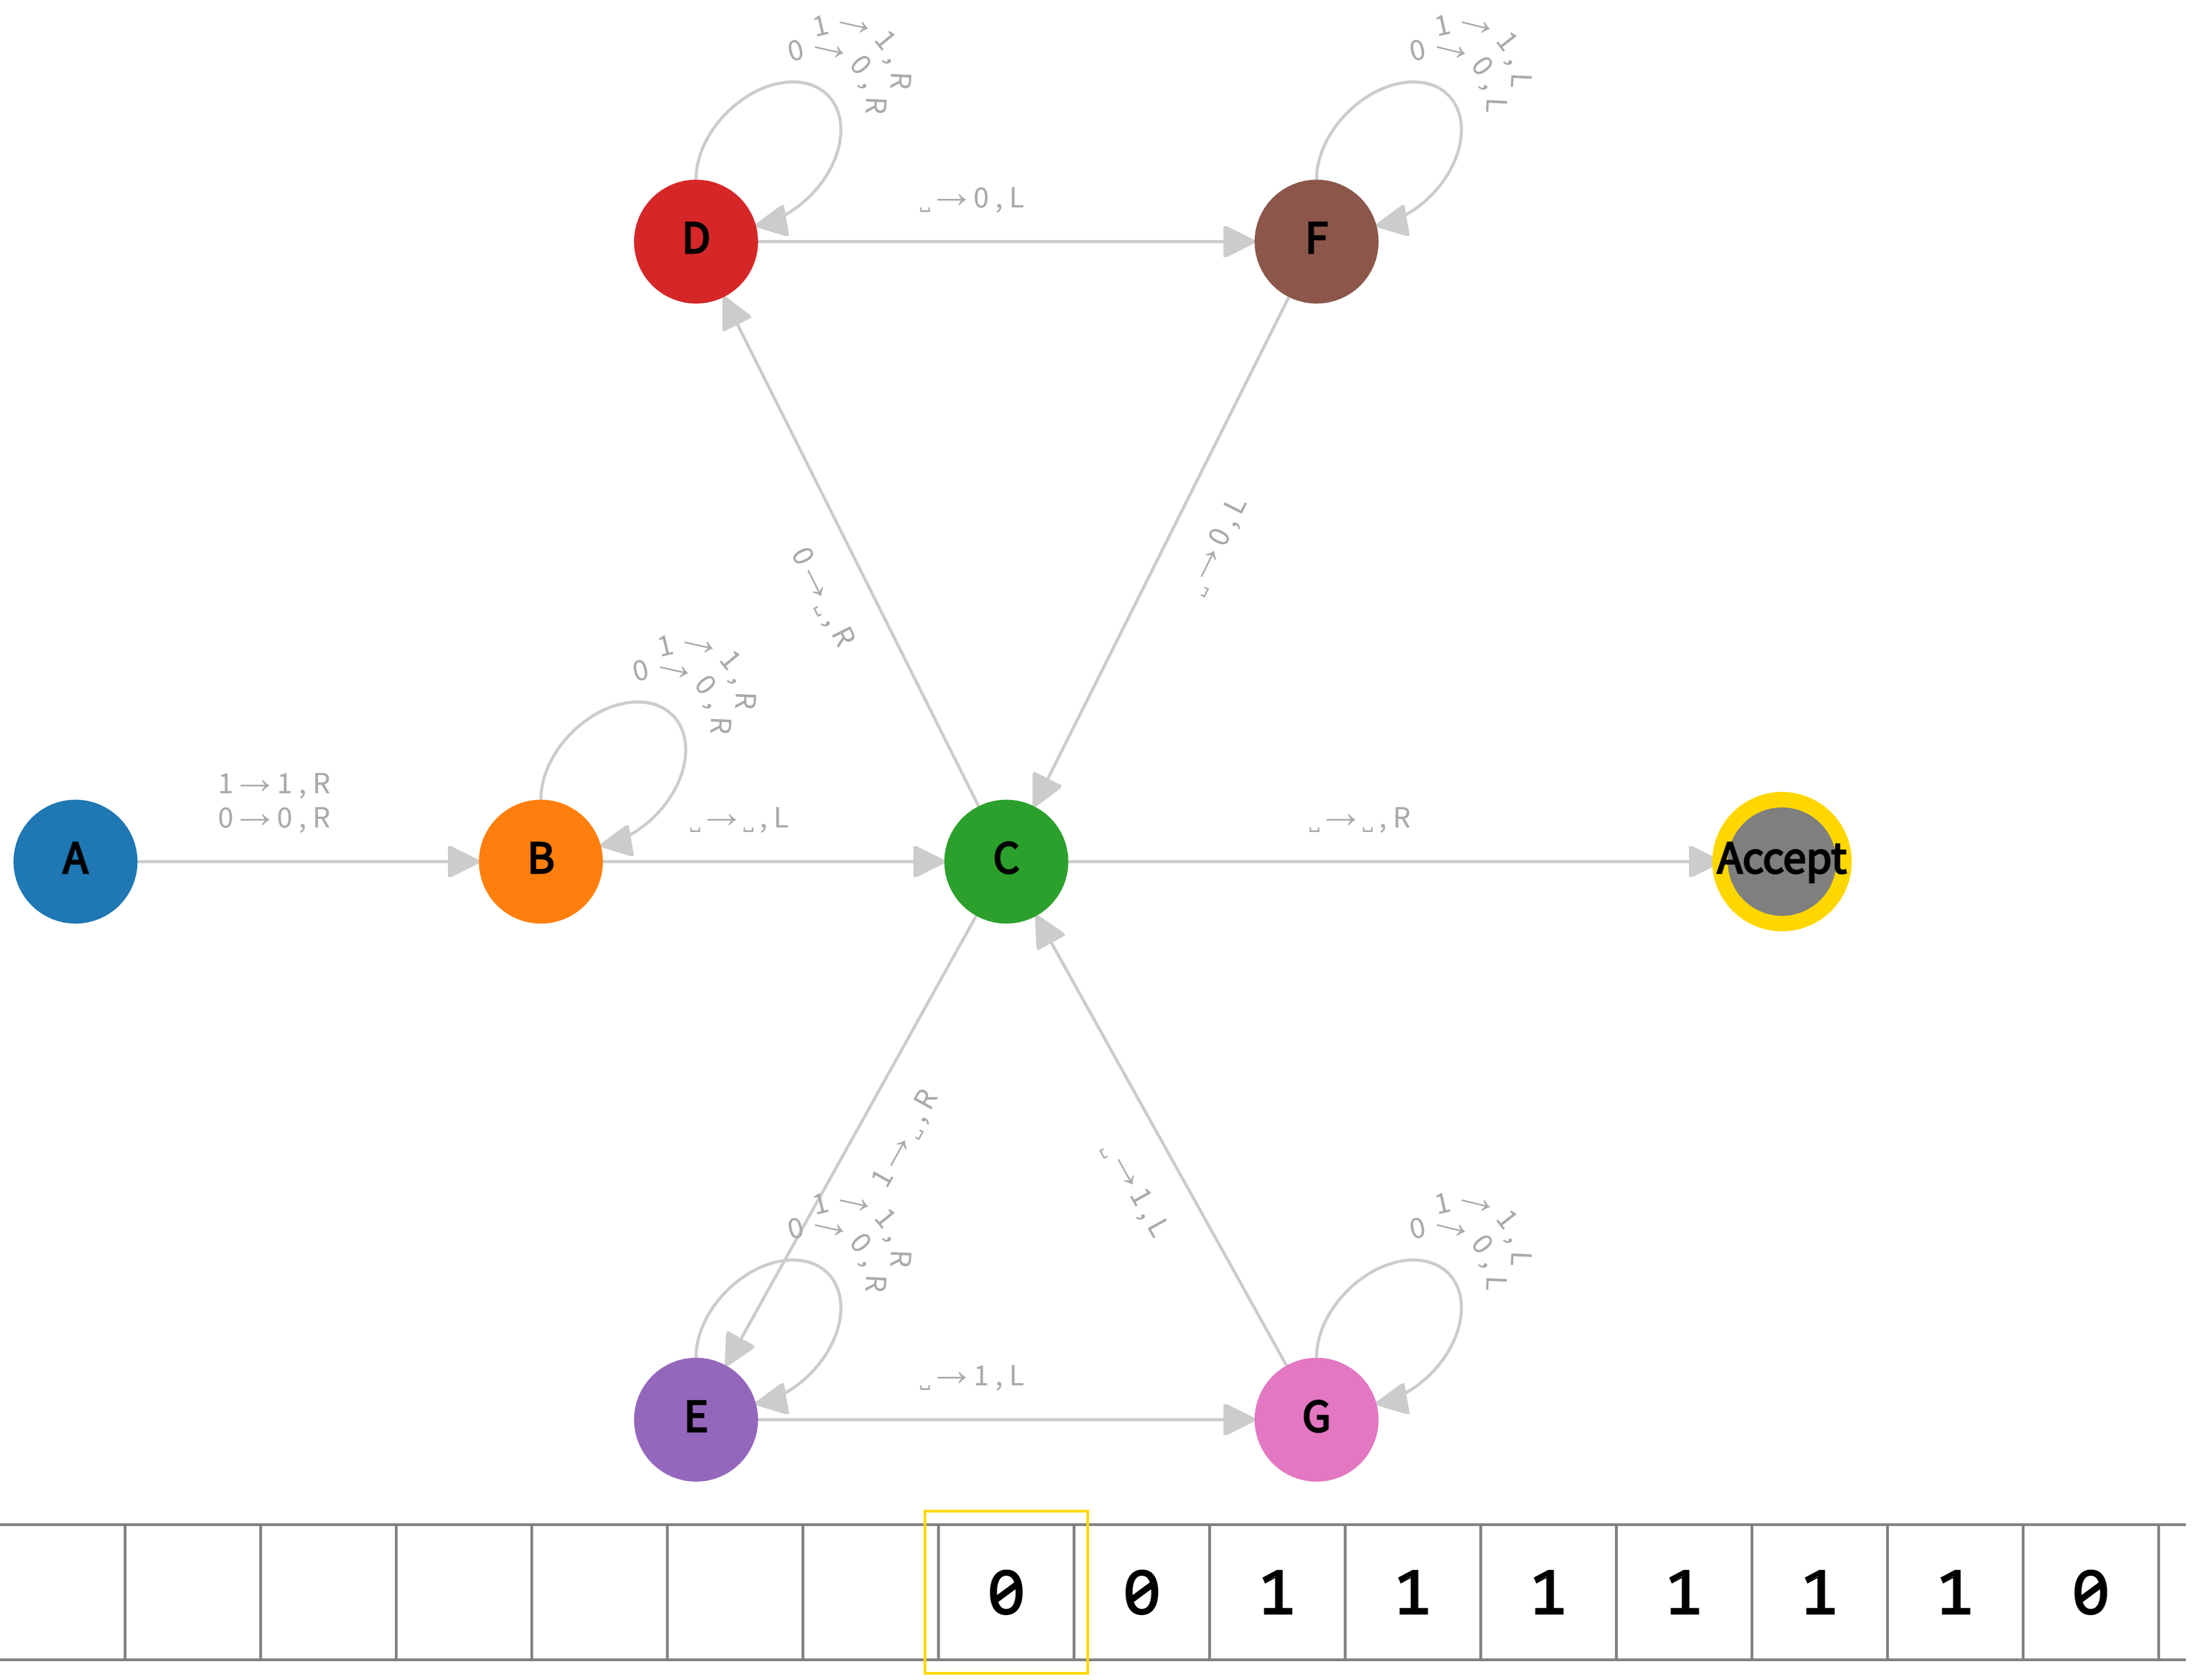
\includegraphics[width=\linewidth]{answers/img/q2-00111-end.png}
    \caption*{Figure (b): End State for $\mathbf{00111}$}
    \label{fig:00111-end}
  \end{minipage}
  \caption{States for $\mathbf{00111}$}
  \label{fig:in-00111}
\end{figure}

\begin{center}
\textbf{\textit{Due to the head place, the whole output cannot be seen in \hyperref[fig:00111-end]{Figure 14.b}.}}
\end{center}

\vspace*{\fill}
\newpage


% General Description

% 1- Scans to the right for first $\blank$. When it is found, move head to left. In other words, find the last symbol in the string.

% 2- Remember the symbol and write $\blank$ and scans to the right for $\blank$. Write symbol to the place instead of $\blank$.

% 3- Scans back to the left for $\blank$ (Lately put). Reinsert the symbol to the place.

% 4- Move head to one left. If it is $\blank$, then stop. If it is a symbol, then repeat 2-4.


\section*{Answer 3}
\label{answer-3}

Let $M_{2D} = (K, \Sigma, \delta, s, H)$ be a 2-dimensional tape where
\begin{itemize}
  \item $K$ is the finite set of states
  \item $\Sigma$ is the input alphabet with $\blank$
  \item $s \in K$, initial state
  \item $H \subseteq K$, halting states
  \item $\delta\ :\ ( (K - H) \times \Sigma) \mapsto K \times ( \Sigma \cup \{ \la, \ra, \uparrow, \downarrow \} )$ is the transition function.
\end{itemize}

\subsection*{Configuration}
\label{q3-configuration}

\begin{itemize}
  \item Let the input string $w$ be of the form:
    \begin{table}[ht]
      \centering
      \begin{tabular}{rcccc}
                  & $\triangledown$ & $\triangledown$ & $\triangledown$ & $\cdots$  \\
        $\tar$    & $w_{11}$        & $w_{12}$        & $w_{13}$        & $\cdots$  \\
        $\tar$    & $w_{21}$        & $w_{22}$        & $w_{23}$        & $\cdots$  \\
        $\tar$    & $w_{31}$        & $w_{32}$        & $w_{33}$        & $\cdots$  \\
        $\vdots$  & $\vdots$        & $\vdots$        & $\vdots$        & $\ddots$  \\
      \end{tabular}
    \end{table}
  \item Also, let the $i^{th}$ row is denoted as $w_i$, $j^{th}$ column is denoted as $w_j$ and let $\underline{w_{ij}}$ show that head of tape is on symbol $w_{ij}$.
\end{itemize}

\noindent So, configuration can be shown as follows,
\begin{center} % Configuration
$\left( q, 
  \begin{tabular}{rccccc}
            & $\triangledown$ & $\triangledown$ & $\triangledown$       & $\triangledown$  & $\cdots$  \\
  $\tar$    & $w_{11}$        & $\cdots$        & $w_{1j}$              & $\cdots$         & $\cdots$  \\
  $\tar$    & $\vdots$        & $\ddots$        & $\cdots$              & $\cdots$         & $\cdots$  \\
  $\tar$    & $w_{i1}$        & $\vdots$        & $\underline{w_{ij}}$  & $\cdots$         & $\cdots$  \\
  $\vdots$  & $\vdots$        & $\vdots$        & $\vdots$              & $\ddots$         & $\cdots$  \\
  $\vdots$  & $\vdots$        & $\vdots$        & $\vdots$              & $\vdots$         & $\ddots$  \\
  \end{tabular}
\right)$
or
$\left( q, \sigma \right)$
\end{center}
where $q$ is the state of the machine, $\sigma$ is the symbol that is located on $w_{ij}$ and head is on the $w_{ij}$.

\noindent As an example, consider the following:
\begin{center} % Example Configuration
$\left( q, 
  \begin{tabular}{rccc}
            & $\triangledown$ & $\triangledown$       & $\triangledown$ \\
  $\tar$    & $a$             & $a$                   & $b$             \\
  $\tar$    & $a$             & $\underline{b}$       & $a$             \\
  $\tar$    & $b$             & $b$                   & $b$             \\
  \end{tabular}
\right)$
\end{center}
where $q$ is the state of the machine, the symbol that is located on $w_{ij}$ is $b$ and head is on the this $b$.


\subsection*{Computation}
\label{q3-computation}

\noindent Computation may be done as follows:
\begin{center} % Computation
$\left( q, 
  \begin{tabular}{rccccc}
            & $\triangledown$ & $\triangledown$ & $\triangledown$       & $\triangledown$  & $\cdots$  \\
  $\tar$    & $w_{11}$        & $\cdots$        & $w_{1j}$              & $\cdots$         & $\cdots$  \\
  $\tar$    & $\vdots$        & $\ddots$        & $\cdots$              & $\cdots$         & $\cdots$  \\
  $\tar$    & $w_{i1}$        & $\vdots$        & $\underline{w_{ij}}$  & $\cdots$         & $\cdots$  \\
  $\vdots$  & $\vdots$        & $\vdots$        & $\vdots$              & $\ddots$         & $\cdots$  \\
  $\vdots$  & $\vdots$        & $\vdots$        & $\vdots$              & $\vdots$         & $\ddots$  \\
  \end{tabular}
\right)
\vdash_{M_{2D}}
\left( p, 
  \begin{tabular}{rccccc}
            & $\triangledown$ & $\triangledown$ & $\triangledown$       & $\triangledown$  & $\cdots$  \\
  $\tar$    & $w_{11}$        & $\cdots$        & $w_{1j}$              & $\cdots$         & $\cdots$  \\
  $\tar$    & $\vdots$        & $\ddots$        & $\cdots$              & $\cdots$         & $\cdots$  \\
  $\tar$    & $w_{i1}$        & $\vdots$        & $\underline{w_{ij}'}$ & $\cdots$         & $\cdots$  \\
  $\vdots$  & $\vdots$        & $\vdots$        & $\vdots$              & $\ddots$         & $\cdots$  \\
  $\vdots$  & $\vdots$        & $\vdots$        & $\vdots$              & $\vdots$         & $\ddots$  \\
  \end{tabular}
\right)$
where
$\delta(q, w_{ij}) = (p, w_{ij}')$
\end{center}

\noindent As an example, consider the following:
\begin{center} % Example Computation 1
$\left( q, 
  \begin{tabular}{rccc}
            & $\triangledown$ & $\triangledown$       & $\triangledown$ \\
  $\tar$    & $a$             & $a$                   & $b$             \\
  $\tar$    & $a$             & $\underline{b}$       & $a$             \\
  $\tar$    & $b$             & $b$                   & $b$             \\
  \end{tabular}
\right)
\vdash_{M_{2D}}
\left( q, 
  \begin{tabular}{rccc}
            & $\triangledown$ & $\triangledown$       & $\triangledown$ \\
  $\tar$    & $a$             & $a$                   & $b$             \\
  $\tar$    & $a$             & $\underline{a}$       & $a$             \\
  $\tar$    & $b$             & $b$                   & $b$             \\
  \end{tabular}
\right)$
where $\delta(q, b) = (p, a)$
\end{center}

\begin{center} % Example Computation 2
  $\left( q, 
    \begin{tabular}{rccc}
              & $\triangledown$ & $\triangledown$       & $\triangledown$ \\
    $\tar$    & $a$             & $a$                   & $b$             \\
    $\tar$    & $a$             & $\underline{b}$       & $a$             \\
    $\tar$    & $b$             & $b$                   & $b$             \\
    \end{tabular}
  \right)
  \vdash_{M_{2D}}
  \left( q, 
    \begin{tabular}{rccc}
              & $\triangledown$ & $\triangledown$       & $\triangledown$ \\
    $\tar$    & $a$             & $a$                   & $b$             \\
    $\tar$    & $a$             & $\underline{\blank}$       & $a$             \\
    $\tar$    & $b$             & $b$                   & $b$             \\
    \end{tabular}
  \right)$
where $\delta(q, b) = (p, \blank)$
\end{center}


\subsection*{Meaning of Deciding a Language $L$}

\noindent Deciding a language $L$ for such a machinev $M$ is the following:
\begin{quote}
  If $\Sigma_0 \subseteq \Sigma - \{ \blank, \tar \}$ is an alphabet and $L$ is a language such that $L \subseteq \Sigma_0^*$. It is said that $M$ decides a language $L$ if one of the followings is true for any string $w \in \Sigma_0^*$:
  \begin{itemize}
    \item $w \in L$ $\Rightarrow$ $M$ accepts $w$.
    \item $w \notin L$ $\Rightarrow$ $M$ rejects $w$.
  \end{itemize}
\end{quote}


\subsection*{Showing that simulating $t$ steps is polynomial in t and n.}

In order to simulate $t$ steps of $M_{2D}$, first $2D$ input should be written on a $1D$ tape with a special character, let say $\$$, such that:

\begin{figure}[ht]
  \centering
  \begin{minipage}{.3\linewidth}
    \centering
    \caption*{\underline{$M_{2D}$ tape}}
    \begin{tabular}{rcccc}
                & $\triangledown$ & $\triangledown$ & $\triangledown$ & $\triangledown$   \\
      $\tar$    & $a$             & $b$             & $a$             & $a$               \\
      $\tar$    & $b$             & $a$             &                 &                   \\
      $\tar$    & $b$             & $b$             &                 &                   \\
      $\vdots$  &                 &                 &                 &                   \\
    \end{tabular}
  \end{minipage}
  \begin{minipage}{.15\linewidth}
    \caption*{\underline{$M_{1D}$ tape}}
    \begin{equation*}
      {\tar}abaa\$ba\$bb\ldots
    \end{equation*}
  \end{minipage}
\end{figure}

\noindent Based on this scheme $t$ steps can be simulated in polynomial time such that:
\begin{itemize}
  \item $\la (\textbf{L}eft)$: Left move in $1D$ is similar to in $2D$ except:
    \begin{quote}
      On $2D$ tape, if head is on left boundary and tries to move left, it will stay put. On $1D$ tape, if $\$$ is read while moving left it will stay out instead. 
    \end{quote}
  \item $\ra (\textbf{R}ight)$: Right move in $1D$ is similar to in $2D$ except:
    \begin{quote}
      On $2D$ tape, if head moves the $\textbf{R}ight$ to the end of the input, content of $1D$ tape should be shifted from that point (in order to insert $\blank$'s that are not shown.)
    \end{quote}
  \item $\uparrow (\textbf{U}p)$: Up move can be implemented such that count the distance from the closest $\$$ on the left, then find the cell having similar distance from its $\$$.
  
    For ceiling boundary and tries to move $\uparrow$, it will stay put. In $1D$ tape, if the tape head is on cells before $\$$ character, no transition need to be defined.
  \item $\downarrow (\textbf{D}own)$: Similar to $\uparrow$.
\end{itemize}

\noindent All actions can be simulated in polynomial time since for a given action, at every step of the simulation either a constant time operation or $O(n^k)$ times for some $k \geq 1$. So, $t$ steps of $M_{2D}$ can be achieved in $t \cdot O(n^k)$ which is polynomial in $t$ and $n$.


\end{document}
